\documentclass[whitelogo]{TUD-report2020}
\usepackage[style=ieee]{biblatex}
\addbibresource{report.bib}
\usepackage{changes}
\usepackage[dutch]{babel}
\usepackage{pgfgantt}
\usepackage{rotating}
\usepackage{fancyhdr}
\usepackage{float}
\usepackage{booktabs}
\usepackage{xcolor}
\usepackage{colortbl}
\usepackage{pgfplots}
\pgfplotsset{compat=1.18}
\usepackage{pgfplotstable}
\usepackage{tikz}
\usetikzlibrary{patterns, calc, intersections}
\usepgfplotslibrary{fillbetween}
\usepackage{placeins}
\usepackage{amssymb}
\usepackage{amsmath, booktabs, float, xcolor, colortbl}
\usepackage{tikz, pgfplots}
\usetikzlibrary{arrows.meta, calc, positioning, patterns, fillbetween}
\pgfplotsset{compat=1.18}
\usepackage{pifont}   % voor \cmark / \xmark
\newcommand{\cmark}{\ding{51}}
\newcommand{\xmark}{\ding{55}}

\newcommand{\cmark}{\tikz\draw[scale=0.3] (0,0) -- (0.2,-0.2) -- (0.6,0.2);}



\fancypagestyle{mainmatter}{%
    \fancyhf{}                    % clear all header and footer fields
    \fancyfoot[C]{\titlefont\thepage}  % page number at center bottom
    \renewcommand{\headrulewidth}{0pt} % remove header line
    \renewcommand{\footrulewidth}{0pt} % remove footer line
}

% Chapter starting pages (plain) also at bottom
\fancypagestyle{plain}{%
    \fancyhf{}
    \fancyfoot[C]{\titlefont\thepage}  % bottom center
    \renewcommand{\headrulewidth}{0pt}
    \renewcommand{\footrulewidth}{0pt}
}

% Apply to all pages
\pagestyle{mainmatter}

\begin{document}
\pagenumbering{arabic}

%% Use Roman numerals for the page numbers of the title pages and table of
%% contents.
\frontmatter

%% Uncomment following 19 lines for a cover with a picture on the lower half only
%\title[tudelft-white]{Title}
%\subtitle[tudelft-cyan]{Optional subtitle}
%\author[tudelft-white]{J.\ Random}
%\affiliation{Technische Universiteit Delft}
%\coverimage{cover.jpg}
%\titleoffsetx{10cm}
%\titleoffsety{10cm}
%\afiloffsetx{1cm}
%\afiloffsety{18cm}
%\covertext[tudelft-white]{
%    \textbf{Cover Text} \\
%    possibly \\
%    spanning 
%    multiple 
%    lines
%    \vfill
%    ISBN 000-00-0000-000-0
%}
%\makecover

%% Uncomment following 16 lines for a cover with a picture on the lower half only
\title[tudelft-white]{BEP}
\subtitle[tudelft-black]{Verduurzaming Jansje}
\affiliation{Technische Universiteit Delft}
\coverimage{fotovanjansje.jpg}
\covertext[tudelft-white]{
    \begin{minipage}[t]{0.48\textwidth}
        \textbf{Groepsleden:} \\
        M.D. Aarts \\
        C.S. Kalkman \\
        A. el Moubarik \\
        Z.R. Neuteboom \\
        S.J.J. Pufe
    \end{minipage}%
    \hfill
    \begin{minipage}[t]{0.48\textwidth}
        \textbf{Projectbegeleiders:} \\
        Jeroen Pruijn \\
        Hans Visser
    \end{minipage}
}
\setpagecolor{tudelft-cyan}
\makecover[split]
\begin{titlepage}

\begin{center}

%% Insert the TU Delft logo at the bottom of the page.

%% Print the title in cyan.
{\makeatletter
\largetitlestyle\fontsize{64}{94}\selectfont\@title
%\largetitlestyle\color{tudelft-cyan}\Huge\@title
\makeatother}

%% Print the optional subtitle in black.
{\makeatletter
\ifx\@subtitle\undefined\else
    \bigskip
   {\tudsffamily\fontsize{22}{32}\selectfont\@subtitle}    
    %\titlefont\titleshape\LARGE\@subtitle
\fi
\makeatother}

\bigskip
\bigskip

door

\bigskip
\bigskip

{\makeatletter
\largetitlestyle\fontsize{26}{26}\selectfont 
\textbf{Groep 05}\\
\vspace{7mm}
M.D. Aarts (6044905) \\ 
C.S. Kalkman (5845394) \\ 
A. El Moubarik (5597617) \\ 
Z.R. Neuteboom (6010253) \\ 
S.J.J. Pufe (6071082)
\makeatother}


\bigskip
\bigskip


\vfill

\begin{tabular}{lll}
    Projectduur: & \multicolumn{2}{l}{9 februari 2026 -- 12 juni 2026} \\
    Projectbegeleider: & Prof.\ dr.\ ir.\ J.\ Pruijn, & TU Delft, supervisor \\
        & Dhr.\ H.\ Visser, & Kwartiermaker Project Maassluis\\
        & Dhr.\ W. van Baalen\ , & Waarnemend eigenaar Jansje
\end{tabular}

\bigskip
\bigskip
\emph{}

\bigskip
\bigskip
%\\[1cm]

%\centering{
\includegraphics{cover/logo_black}}


\end{center}
\begin{tikzpicture}[remember picture, overlay]
    \node at (current page.south)[anchor=south,inner sep=0pt]{
        
\includegraphics{cover/logo_black}
    };
\end{tikzpicture}

\end{titlepage}

\mainmatter
\let\cleardoublepage\clearpage


\chapter*{Samenvatting}
\setheader{Preface}

In samenwerking met loods M en haar stakeholders, zal een ontwerp gerealiseerd worden voor het historische transportschip Jansje. Hierbij is de harde eis dat de aandrijving in het nieuwe ontwerp draait op volledig hernieuwbare energie. Om tot dit ontwerp te komen, is eerst gekeken naar het vaarprofiel, en welke technische parameters hieruit voortvloeien. Door middel van een interview met de waarnemend eigenaar van Jansje is het operationeel profiel vastgesteld. 
\\\\
Daarna is er onderzoek gedaan naar de verschillende mogelijkheden voor energieopslagsystemen voor hernieuwbare energie. Dit is gedaan door middel van een uitgebreide literatuurstudie, een model, technische criteria en maatschappelijk relevante criteria. Er is gekeken naar zowel bestaande als nog experimentele techniek. De uitkomst hiervan is dat een combinatie van experimentele zeezoutbatterijen met lithium-ion batterijen de meest geschikte energiebron zal zijn. 
\\\\
Als laatst is onderzocht welke aandrijving het beste past bij het operationeel profiel van Jansje en de gekoze energiebron. Hieruit is voortgekomen dat een elektrische motor het meest geschikt is. Omdat er vele elektromotoren beschikbaar zijn, is ervoor gekozen om niet één elektromotor aan te bevelen, maar in plaats daarvan een set criteria mee te geven, waarmee er ten tijde van de daadwerkelijke implementatie de keuze gemaakt kan worden.




\tableofcontents

\chapter{Inleiding}

Dit rapport heeft als doel om te onderzoeken op welke manier Jansje op een technisch en financieel haalbare wijze  kan worden verduurzaamd. Dit wordt gedaan in samenwerking met Loods M en andere betrokken stakeholders. De bijdrage van het vervoer over water aan de totale CO$_2$-uitstoot door de Nederlandse economie was bijna 7\% \cite{cbs_water_uitstoot}. Het verduurzamen van schepen zal een belangrijke bijdrage leveren aan het behalen van de klimaatdoelstellingen voor 2050 \cite{imo_ghg_emissions}. \\

\noindent
Loods M is een Fieldlab in Maassluis dat op zoek is naar innovatieve ideeën om schepen te verduurzamen. In Loods M komen studenten, vakmensen en bedrijven samen om slimme ideeën in het echte leven te testen. Eén van de schepen binnen dit project is Jansje. Jansje is een historisch transportschip dat in Maassluis ligt en in 1899 is gebouwd \cite{Jansje}. Het schip is al vijf generaties in bezit van dezelfde familie. Op dit moment heeft Jansje een conventionele dieselmotor, wat valt onder de stage 1b \cite{dieselnet_eu_nonroad_standards}. Deze aandrijving leidt tot de uitstoot van relatief veel emissiegassen. Het verduurzamen van dit schip vormt daarom een relevante technische en maatschappelijke uitdaging. Er worden verschillende aandrijvingen en energiedragers onderzocht om de meest geschikte keuze te maken voor Jansje.\\


\noindent Fieldlab Maassluis heeft samenwerkingen met verschillende bedrijven, echter is niet elk bedrijf relevant in dit onderzoek. Bedrijven die wel relevant zijn, zijn Dr Ten \cite{drten_zeezout_batterij2} die een Zeezoutbatterij zouden kunnen leveren, Nedstack \cite{nedstack_pem_fuel_cell_stacks} die beschikking hebben tot een waterstof brandstofcel. Ook worden er nog andere bedrijven gecontacteerd, voor de nodige informatie. Het onderzoek zal worden gedaan voor het fieldlab en dat zal betekenen dat de voorzieningen van deze bedrijven zullen worden onderzocht maar niet verplicht zijn om te gebruiken.


\chapter{Onderzoeksaanpak}
Eerst zal begonnen worden met het vaststellen van het operationeel profiel van Jansje. Hiervoor is de eigenaar geïnterviewd en die gaf alle benodigde informatie. Ook zullen enkele kleine berekeningen gemaakt worden om te bepalen hoeveel vermogen en capaciteit er nodig is voor de hotel-load.
\\\\
Om het energieopslagsysteem voor het schip te kunnen maken, wordt eerst literatuuronderzoek gedaan naar de verschillende mogelijkheden. Met behulp van een excel-model en meerdere criteriatabellen zal de keuze gemaakt worden welk energieopslagsysteem het meest geschikt is. Hiervoor wordt met de Holtrop-Mennen methode de scheepsweerstand berekend, en daarna verder gerekend om het minimaal te installeren motorvermogen te berekenen. Samen met het energieverbruik dat uit het operaitoneel profiel voorkomt, kan nu bepaald worden hoeveel energie constant geleverd moet worden tijdens het varen.
\\\\
Voordat er verder ingegaan wordt op het energieopslagsysteem, wordt eerst nog gekeken naar randvoorwaarden. Deze zijn van belang voor de totale hoeveelheid energie die op het schip opgeslagen moet worden. 
\\\\
Vervolgens zal een keuze worden gemaakt voor de meest geschikte energieopslag. Deze keuze wordt gemaakt door middel van modellen, een stroomschema en meerdere criteria.
\\\\
Nu de energieopslag bekend is, kan gekeken worden naar het aandrijfsysteem. Vanuit het operationeel profiel en het gekozen energieopslagsysteem zijn parameters zoals het vermogen en toerental bepaald. Omdat er veel verschillende motoren op de markt zijn, wordt niet gekeken naar één specifieke aandrijving, maar meer naar de parameters waaraan de motor moet voldoen.
\\\\
Als alle onderdelen bekend zijn, wordt door middel van een stabiliteitsberekening gekeken hoe en waar alle onderdelen het best geplaatst kunnen worden om de gewilde eigenschappen te verkrijgen. Tevens wordt gecheckt of het nieuwe gewicht acceptabel is voor het schip.
\\\\
Parallel aan de stabiliteits- en massaberekeningen, is een experiment gedaan met de nog experimentele zeezoutbatterij, om te kijken hoe deze reageert op karakteristieke golfbewegingen waar het in een schip aan blootgesteld wordt.
\\\\
Als laatste wordt afgesloten met meerdere ontwerpen voor de implementatie van het nieuwe systeem in de Jansje. Hiervoor wordt ook rekening gehouden met veiligheid. Hieruit wordt het beste ontwerp gekozen, en deze zal worden voorgelegd aan W. van Baalen als meest geschikte ontwerp om te omplementeren in de Jansje.

\begin{figure}[h]
    \centering
    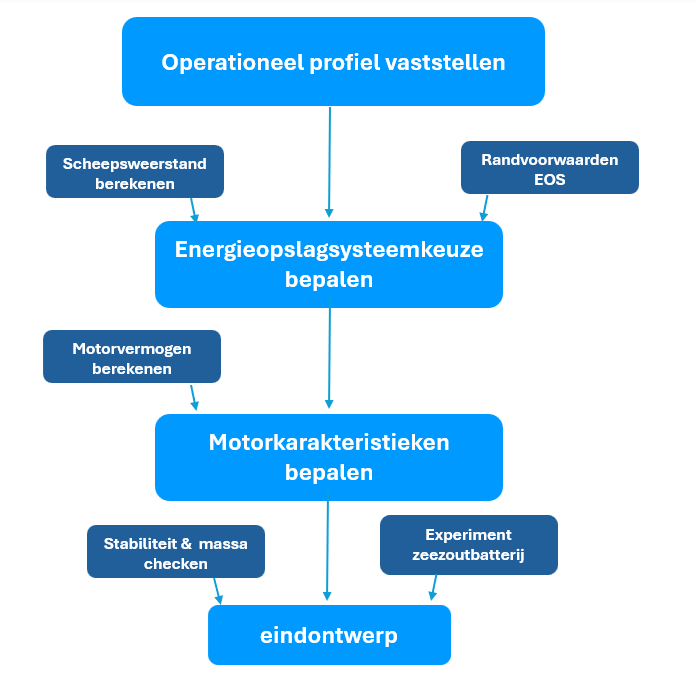
\includegraphics[width=0.8\linewidth]{chart V1.png}
    \caption{Stroomschema van dit project.}
    \label{fig:zijkant}
\end{figure}

\chapter{Probleemdefinitie en aanpak}

\section{Probleemdefinitie}
Het doel van dit project is om te onderzoeken hoe het schip Jansje, een historisch transportschip, in de nabije toekomst kan worden verduurzaamd. Hierbij moet rekening gehouden worden met de eisen van de eigenaar van het schip en het Fieldlab Maassluis. Daarnaast moet er gebruikgemaakt worden van groene energie. De opdracht is volbracht als het eindrapport een concreet ontwerpvoorstel bevat voor een duurzame aandrijflijn dat voldoet aan de eisen die gesteld zijn door de eigenaar van Jansje en Fieldlab Maassluis. Concreet betekent dit: 
\begin{itemize}
    \item Een onderbouwde systeemkeuze op basis van een gewogen criteriatabel \cite{Triantaphyllou2000}.
    \item Een energieberekening die aantoont dat de vereiste actieradius haalbaar is.
    \item Een stabiliteitsanalyse die bevestigt dat het schip veilig en efficiënt kan blijven functioneren met het nieuwe systeem.
    \item Een CAPEX/OPEX berekening om te zien of het voorstel financieel haalbaar is
    \item 
    Het voorstel kan voldoen aan de gestelde wet \& regelgeving
\end{itemize}


\section{Belangrijkste uitdagingen \& afbakening}

\subsection{Belangrijkste uitdagingen}
\begin{itemize}

\item \textbf{Wat zijn de financiële parameters voor dit project?} \\
    Bij dit project wordt onder andere gekeken naar duurzame (experimentele) energieopslag. Dit is relatief duur ten opzichte van traditionele energieopslag, dus is het belangrijk om te weten welke financiële eisen er zijn voor dit project. Naast het ophalen van de financiële eisen bij de opdrachtgever, is de methodologische vraag hier: hoe voeren wordt er een betrouwbare CAPEX/OPEX-analyse uit voor een historisch schip met onconventionele systemen?
\item \textbf{Hoe wordt het operationeel profiel van transportschip Jansje het beste bepaald op een representatieve en reproduceerbare manier?} \\
    Om een goede keuze te kunnen maken voor de aandrijflijn en de benodigde energieopslag, is het van belang om rekening te houden met de operationele eisen. Deze eisen bestaan onder andere uit:
    \begin{itemize}
        \item Het benodigde (piek)vermogen.
        \item De benodigde vaaruren per periode.
        \item Hoelang het schip aan wal ligt.
        \item De gemiddelde vaarsnelheid.
        \item nog meer?
    \end{itemize}
    De uitdaging is voornamelijk hoe het vaarprofiel methodisch te bepalen is. Hiervoor wordt gebruik gemaakt van interviews, logboekanalyses en vaarsimulaties gebaseerd op andere schepen. Op deze manier kunnen deze eisen als betrouwbare randvoorwaarden dienen.
\item \textbf{Hoe wordt bepaald welk energieopslagsysteem het meest geschikt is voor Jansje?}\\
    Hierbij wordt gekeken naar een mogelijke nieuwe energieopslag, dit kan bijvoorbeeld een brandstof, generator, batterij of een combinatie zijn. Verschillende duurzame technologieën worden onderzocht en vergeleken met de op dit moment gebruikelijke technologieën. De eisen die bepaald zijn in het programma van eisen worden vertaald naar gewogen criteria om zo op een zo objectief mogelijke en gewogen manier tot een resultaat te komen.
\item \textbf{Hoe wordt bepaald welke aandrijving het best aansluit bij de gekozen energieopslag?}\\
    Transportschip Jansje heeft bij het kiezen van een nieuw energieopslagsysteem ook een nieuwe aandrijving nodig. De keuze voor de aandrijflijn is afhankelijk van het programma van eisen. Daarnaast hebben de technische specificaties en operationele eisen van het energieopslagsysteem een belangrijke keuze in de overweging. De aandrijvingen die voldoen aan deze eisen en specificaties worden vervolgens vergeleken op basis van prestatie aan de hand van een gewogen criteria analyse. 

\item \textbf{Hoe kan het nieuwe systeem theoretisch optimaal geïmplementeerd worden?}\\
    %Hoe kunnen de nieuwe energieopslag en aandrijving het beste geïmplementeerd worden op Jansje? \\
    Hier wordt onderzocht hoe de combinatie van de energieopslag en de aandrijflijn theoretisch optimaal ingebouwd kan worden in transportschip Jansje om de efficiëntie en stabiliteit van het schip te optimaliseren. Het positioneren van de onderdelen in verschillende configuraties creëert fluctuerende technische specificaties zoals bijvoorbeeld de gewichtsverdeling en vaardiepte. Met deze resultaten kan de weerstand en daarmee het vernieuwde benodigd vermogen van het schip worden bepaald. Via iteraties kan vervolgens de optimale configuratie tussen het energieopslagsysteem en de aandrijfmotor worden bepaald om het schip zo efficiënt mogelijk te maken. Om dit te optimaliseren zal een onderzoek worden gedaan aan de hand van Holtrop-Mennen, een CFD (Computational Fluid Dynamics) analyse of een model experiment.
    
\item \textbf{Hoe kan het nieuwe systeem in de praktijk optimaal geïmplementeerd worden?}\\
    Niet altijd is het theoretische optimum haalbaar. Het is dus van belang om een resultaat te hebben dat in de praktijk te realiseren is. Hierbij wordt rekening gehouden met historische aspecten, veiligheid, en technische haalbaarheid.
    
 \item \textbf{Hoe kan de energiecyclus geoptimaliseerd worden?} \\
   Het energetisch opladen en ontladen is van belang om zo min mogelijk (indirecte) uitstoot te krijgen. Daarnaast is het volume van de energieopslag afhankelijk van hoeveel energie er nodig is, waarmee het optimale gebruik van de energie dus resulteert in het laagste volume voor de energieopslag.
   
\item \textbf{Hoe betrouwbaar is het complete systeem?} \\
    Hier wordt onderzocht wat de levensduur is van het nieuwe systeem en naar de onderhoud die daarvoor nodig zal zijn. Dit is zowel financieel, ecologisch als operationeel van belang. \\  
    
\item \textbf{Hoe voldoet Jansje aan de wet- en regelgeving?} \\
    Het kan zo zijn dat bij bepaalde aandrijflijnen het vaartuig niet voldoet aan alle wettelijke eisen. Het is belangrijk dat Jansje aan de wettelijke eisen voldoet of een uitzonderingstatus krijgt, omdat het schip wel gebruikt moet worden.
\end{itemize}
\subsection{Afbakening}
WILLEN WE DIT?

\section{Hoofd- en deelvragen}

\subsection{Hoofdvraag}
\noindent {Welke duurzame aandrijflijn is volgens de commerciële, technische en maatschappelijke eisen het meest geschikt voor het transportschip “Jansje”?} \\


\subsection{Deelvragen}

\noindent De deelvragen zijn direct afgeleid van de hierboven geïdentificeerde uitdagingen en richten zich niet alleen op het ophalen van kennis, maar ook op de methoden waarmee de antwoorden worden verkregen:

\begin{enumerate}
    \item Hoe wordt het operationeel profiel van Jansje op een representatieve en reproduceerbare wijze vastgesteld?
    \item Welk energieopslagsysteem past het best bij Jansje, gegeven de technische parameters, het operationele profiel en  de financiële parameters?
    \item Welk aandrijfsysteem is het meest geschikt voor transportschip Jansje, rekening houdend met het gekozen energieopslagsysteem en het programma van eisen?
    \item Hoe kan de aandrijflijn worden geïntegreerd in de machinekamer van het schip rekening houdend met ruimte, veiligheid, cultureel erfgoed en regelgeving?
\end{enumerate}

\section{Onderzoeksaanpak}
Eerst zal begonnen worden met het vaststellen van het operationeel profiel van Jansje. Hiervoor is de eigenaar geïnterviewd en die gaf alle benodigde informatie. Ook zullen enkele kleine berekeningen gemaakt worden om te bepalen hoeveel vermogen en capaciteit er nodig is voor de hotel-load.
\\\\
Om het energieopslagsysteem voor het schip te kunnen maken, wordt eerst literatuuronderzoek gedaan naar de verschillende mogelijkheden. Met behulp van een excel-model en meerdere criteriatabellen zal de keuze gemaakt worden welk energieopslagsysteem het meest geschikt is. Hiervoor wordt met de Holtrop-Mennen methode de scheepsweerstand berekend, en daarna verder gerekend om het minimaal te installeren motorvermogen te berekenen. Samen met het energieverbruik dat uit het operaitoneel profiel voorkomt, kan nu bepaald worden hoeveel energie constant geleverd moet worden tijdens het varen.
\\\\
Voordat er verder ingegaan wordt op het energieopslagsysteem, wordt eerst nog gekeken naar randvoorwaarden. Deze zijn van belang voor de totale hoeveelheid energie die op het schip opgeslagen moet worden.
\\\\
Vervolgens zal een keuze worden gemaakt voor de meest geschikte energieopslag. Deze keuze wordt gemaakt door middel van modellen, een stroomschema en meerdere criteria.
\\\\
Nu de energieopslag bekend is, kan gekeken worden naar het aandrijfsysteem. Vanuit het operationeel profiel en het gekozen energieopslagsysteem zijn parameters zoals het vermogen en toerental bepaald. Omdat er veel verschillende motoren op de markt zijn, wordt niet gekeken naar één specifieke aandrijving, maar meer naar de parameters waaraan de motor moet voldoen.
\\\\
Als alle onderdelen bekend zijn, wordt door middel van een stabiliteitsberekening gekeken hoe en waar alle onderdelen het best geplaatst kunnen worden om de gewilde eigenschappen te verkrijgen. Tevens wordt gecheckt of het nieuwe gewicht acceptabel is voor het schip.
\\\\
Parallel aan de stabiliteits- en massaberekeningen, is een experiment gedaan met de nog experimentele zeezoutbatterij, om te kijken hoe deze reageert op karakteristieke golfbewegingen waar het in een schip aan blootgesteld wordt.
\\\\
Als laatste wordt afgesloten met meerdere ontwerpen voor de implementatie van het nieuwe systeem in de Jansje. Hiervoor wordt ook rekening gehouden met veiligheid. Hieruit wordt het beste ontwerp gekozen, en deze zal worden voorgelegd aan W. van Baalen als meest geschikte ontwerp om te omplementeren in de Jansje.

\begin{figure}[h]
    \centering
    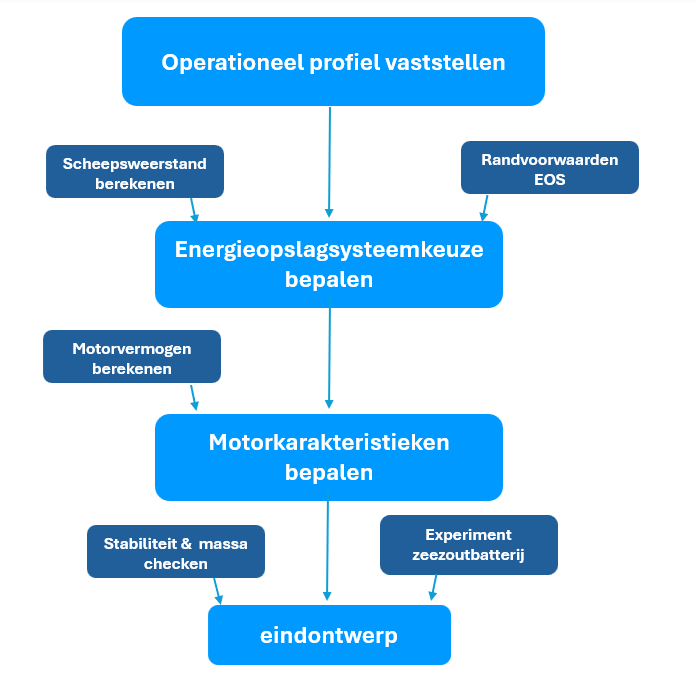
\includegraphics[width=0.8\linewidth]{chart V1.png}
    \caption{Stroomschema van dit project.}
    \label{fig:stroomschema_aanpak}
\end{figure}


\section{Knelpunten, aannames en maatschappelijke aspecten}
\subsection{Knelpunten}
Voor dit project zijn een aantal knelpunten geïdentificeerd.\\

\noindent Allereerst is er beperkt technische data beschikbaar over Jansje. Om deze reden zal er naast de technische data ook data vergaard worden op basis van interviews met de eigenaar en de kapitein, archiefonderzoek en directe opmetingen. Als dit onvoldoende data oplevert, zal worden uitgegaan van referentiewaarden voor vergelijkbare historische binnenvaartschepen uit de literatuur. Dit laatste zal duidelijk aangegeven worden in het verslag.\\

\noindent Ook wordt rekening gehouden met het feit dat stakeholders niet altijd direct zullen reageren. Om te voorkomen dat dit vertraging oplevert, zullen er vroegtijdig plannen gemaakt worden. Daarnaast zal schriftelijke communicatie zo snel als mogelijk verstuurd worden. Bij uitblijven van een respons worden aannames gedaan, gedocumenteerd en voorgelegd tijdens het eerstvolgende contactmoment met de betreffende stakeholders. Eventueel volgt daarna nog een aanpassing in de aannames.\\

\noindent Daarnaast is de verwachting dat er ook gegeken gaat worden naar experimentele technologie, die nog niet is gevalideerd voor nautische applicaties. Aanames die hierbij gemaakt worden, zullen conservatief zijn, en meerdere scenario's zullen worden uitgewerkt.\\

\noindent Als laatste wordt de tijdsdruk bij parallelle deelstudies geïdentificeerd. Om te voorkomen dat deelstudies vastlopen omdat er data en/of conclusies van een parallellopende deelstudies nodig zijn, zullen er wekelijkse meetings plaatsvinden, en duidelijke taken en taakoverdrachten worden gedaan. Als een deelstudie vertraging oploopt, wordt de scope beperkt  tot de voor de energiebalans minimaal benodigde uitvoer. Bijvoorbeeld alleen de kruissnelheid bij de weerstandsberekening in plaats van het volledige vaarprofiel gebruiken.


\subsection{Aannames}
Aannames schrijven die gedaan zijn. BV IN STABILITEIT ETC.


\subsection{Maatschappelijke aspecten}
De gekozen aanpak brengt een aantal maatschappelijke aspecten met zich mee die hieronder worden toegelicht.

\begin{itemize}
    \item \textbf{Veiligheid:} In het ontwerp worden brandveiligheidsmaatregelen meegenomen conform SOLAS-normen \cite{imo_solas_1974} voor kleine schepen. Bij het gebruik van bepaalde brandstofsoorten bestaat explosiegevaar bij lekkage, terwijl batterijsystemen kunnen resulteren in oververhitting en brandgevaar.
    \item \textbf{Duurzaamheid en levenscyclus:} De gebruikte onderdelen in de aandrijflijn worden vergeleken op duurzaamheid. Tevens wordt gekeken naar de levenscyclus van de onderdelen.
    \item \textbf{Ethiek:} Een aantal van de beoogde materialen is schaars en wordt grotendeels gewonnen in landen buiten Europa, waar de werkwijze vaak minder strikt is dan de Europese standaarden \cite{ec_green_claims_2023}  vereisen.
    \item \textbf{Erfgoedwaarde:} Jansje is een historisch schip van grote cultuurhistorische waarde. Ingrijpende veranderingen aan de romp of het interieur kunnen deze waarde aantasten. In overleg met de eigenaar worden aanpassingen zo beperkt mogelijk gehouden; de aandrijflijn en energieopslag worden zo ontworpen dat het historisch karakter van het schip behouden blijft.
\end{itemize}


\section{Leeswijzer}
De rest van het verslag volgt de stappen uit de onderzoeksaanpak. In hoofdstuk 3...
\chapter{Operationeel profiel}


Om het onderzoek wat in dit verslag is beschreven te onderbouwen, is het van belang om het operationeel profiel van transportschip Jansje te bepalen op een manier waar de eigenaar, Wim van Baalen, op kan vertrouwen. Dit sluit aan bij de eerdergenoemde deelvraag 1:

\begin{quote}
    \textit{\textbf{Hoe wordt het operationeel profiel van Jansje op een representatieve en 
    reproduceerbare wijze vastgesteld?}}
\end{quote}

\noindent Om een geschikte, duurzame aandrijflijn voor Jansje te kunnen ontwerpen, moet eerst worden vastgesteld hoe het schip daadwerkelijk wordt gebruikt. Het operationeel profiel beschrijft daarom de frequentie, duur, snelheid, vermogensvraag, hotel-load, financiële randvoorwaarden en meer van het schip. Deze gegevens vormen de basis van het onderzoek naar energieopslagsystemen. Hiervoor wordt eerst de onderzoeksmethode toegelicht. Vervolgens worden het vaarprofiel, het vermogen en energieverbruik, het stilliggen en de laadmogelijkheden, en de belangrijkste randvoorwaarden behandeld.


\section{Onderzoeksmethode}

Om het operationeel profiel te bepalen is een interview gehouden met de eigenaar van Jansje. In combinatie met eerder mailcontact en dit interview is alle benodigde informatie verkregen. Omdat een deel van de gevraagde informatie echter niet direct beschikbaar was, is het operationeel profiel aanvullend onderbouwd aan de hand van vergelijkbare vaartuigen die worden beheerd in de haven van Maassluis door Loods M. De vaartijden van deze schepen zijn openbaar beschikbaar en bieden een representatief referentiekader voor het typische gebruikspatroon van historische vaartuigen in dit vaargebied.

\section{Vaarprofiel}
Het vaarprofiel is bepaald door het interview met de eigenaar. \\
\noindent Uit het inverview \cite{vanbaalen2026interview} zijn de volgende conclusies getrokken:
\begin{itemize}
    \item Het schip vaart tussen mei en oktober.
    \item Het schip vaart ongeveer 30 dagen per jaar.
    \item Een vaartrip duurt gemiddeld 6 uur en maximaal 8 uur.
    \item De gemiddelde vaarsnelheid is 10-12 km/h.
    \item De maximale vaarsnelheid is 14 km/h.
    \item Er is vooral piekvermogen nodig tijdens het wegvaren en aanmeren, en manoeuvreren. Hoevaak dit gedaan moet worden per vaart is voornamelijk afhankelijk van het aantal bruggen dat gepasseerd moet worden.
    \item De routes zijn willekeurig. 
    \item De boot gaat naar events waar ze uitgenodigd worden, van Amsterdam tot Dordrecht, overal in Nederland.
\end{itemize}


\section{Vermogen en energieverbruik}
\subsection{Piekvermogen en manoeuvreren}

De boot wordt op dit moment aangedreven door een motor van 100pK van General Motors \cite{Jansje}. Omgerekend is dat bijna 80 kW. Verder is de hotel-load bestaat uit alle elektriciteitconsumerende apparaten aan boord die geen onderdeel zijn van de aandrijflijn.
Uit het interview en een rondleiding is de conclusie getrokken dat hier rekening mee gehouden moet worden.
\noindent Uit het interview bleek ook dat er bepaalde apparaten aanwezig zijn op het schip die vallen onder de Hotel load:
\begin{itemize}
    \item Verlichting
    \item Koelkast
    \item Navigatie
    \item Koken
    \item Boiler
\end{itemize}

\section{Stilliggen en laadmogelijkheden}
Tijdens het interview is naar voren gekomen dat met transportschip Jansje ook naar events wordt gevaren verder in het land. Voor bijvoorbeeld SAIL in Amsterdam, wordt dan twee dagen achtereenvolgend gevaren met Jansje. De eigenaar van Jansje heeft aangegeven dat de vaartijd van acht uur per dag een goede indicatie is, en dat ervan uitgegaan kan worden dat er een elektriciteits aansluiting van 230V beschikbaar is als het schip ligt aangemeerd.\\



\section{Resultaten}

In deze paragraaf zijn de parameters van het operationeel profiel uitgezet:

\begin{table}[H]
    \centering
    \caption{Geregistreerde vaartijden van referentieschepen beheerd door Loods M te Maassluis}
    \label{tab:vaartijden}
    \begin{tabular}{llll}
        \toprule
        \midrule
        \textbf{Vaarprofiel \& routes} & \\
        \midrule
        \bottomrule
        Hoeveel vaart jansje per jaar? & 30 dagen \\
        Hoeveel uur vaart Jansje gemiddeld? & 6-8 uur \\
        wat is de gemiddelde vaarsnelheid? & 10-12 km/h \\
        Welke afstand vaart jansje gemiddeld? & 36-80 km\\
        
        \toprule
        \midrule
        \textbf{Vermogen \& energieverbruik} & \\
        \midrule
        \bottomrule
        Wat is het piekvermogen van de oude motor? & 100pk (73.55 kW)\\
        Hoeveel piekvermogen is er nodig tijdens het varen? & ??\\
        Wat is de geschatte hotel-load? & ??\\
        
        \toprule
        \midrule
        \textbf{Stilligen \& Laadmogelijkheden} & \\
        \midrule
        \bottomrule
        Hoelang ligt het schip aan wal? & ??\\
        op welke krachtstroom kan geladen worden aan wal? & ??\\
        \toprule
        \midrule
        

        
    \end{tabular}
\end{table}




\section{Conclusie}

Met deze resultaten kan de conclusie worden getrokken dat het operationeel profiel succesvol is bepaald. Met deze resultaten kunnen de eisen, zoals later specifiek beschreven bij de verschillende deelvragen, worden opgesteld.
 
% ============================================================


\chapter{Weerstandsschatting en aandrijflijn}
\label{ch:holtrop-aandrijflijn}

\noindent In dit hoofdstuk wordt deelvraag 2 beantwoord:

\begin{quote}
    \textit{\textbf{Welk energieopslagsysteem past het best bij Jansje, gegeven de
    technische parameters, het operationele profiel en de financiële parameters?}}
\end{quote}

\noindent Hiervoor is het benodigd aandrijfvermogen een belangrijke
invoerparameter. Om deze te verkrijgen, wordt eerst de scheepsweerstand geschat via de
Holtrop-Mennen methode. Daarna wordt de volledige aandrijflijn doorgerekend naar
het minimaal te installeren motorvermogen.

% ============================================================
\section{Weerstandsschatting met de Holtrop-Mennen methode}
\label{sec:holtrop}

De totale weerstand van \emph{'t~Jansje} in varende conditie is bepaald met de
statistische regressiemethode van Holtrop en Mennen \cite{Holtrop1984}. De methode
gaat uit van diepwater bij zeewater ($\rho = 1025\ \mathrm{kg/m^3}$,
$15\,^{\circ}\mathrm{C}$) en kalm water. Omdat \emph{'t~Jansje} op binnenwateren
vaart levert dit een conservatieve schatting; de bijbehorende beperkingen worden
behandeld in Sectie~\ref{subsec:holtrop-validatie}.

De totale weerstand is opgebouwd uit de volgende componenten \cite{Holtrop1984}:

\begin{equation}
    R_\mathrm{totaal} = R_F(1+k_1) + R_{APP} + R_W + R_B + R_{TR} + R_A
    \label{eq:Rtot}
\end{equation}

\noindent waarbij $R_F$ de wrijvingsweerstand is volgens de ITTC-1957 formulering,
$(1+k_1)$ de visceuze vormfactor van de romp, $R_{APP}$ de aanhangselweerstand,
$R_W$ de golfweerstand, $R_B$ en $R_{TR}$ resp.\ boegbulb- en spiegelweerstand,
en $R_A$ de modelschaalkorrelatieallowance. De wrijvingsweerstand volgt uit:

\begin{equation}
    R_F = \tfrac{1}{2}\,\rho\,V^2\,S\,C_F, \qquad
    C_F = \frac{0{,}075}{(\log Re - 2)^2}
    \label{eq:RF}
\end{equation}

De overige componenten worden berekend via regressieformules in de scheepsparameters
$L_{wl}$, $B$, $T$, $C_B$, $C_P$, $C_{WP}$, $C_M$ en $L_{CB}$; de volledige
uitwerking is geïmplementeerd in de spreadsheet \cite{spreadsheet_holtrop}.

% ------------------------------------------------------------------
\subsection{Scheepsgegevens}
\label{subsec:holtrop-scheepsgegevens}

\begin{table}[H]
\centering
\caption{Invoerparameters Holtrop-schatting, \emph{'t~Jansje} (varende conditie)}
\label{tab:holtrop_input}
\begin{tabular}{llll}
\toprule
Parameter & Symbool & Waarde & Eenheid \\
\midrule
Lengte waterlijn            & $L_{wl}$    & 22{,}22 & m        \\
Breedte waterlijn           & $B$         &  4{,}36 & m        \\
Diepgang voor- en achterschip & $T$       &  1{,}50 & m        \\
Verdringingsvolume          & $\nabla$    & 73{,}0  & m$^3$    \\
Hoofdspantcoëfficiënt       & $C_M$       &  0{,}90 & --       \\
Waterplancoëfficiënt        & $C_{WP}$    &  0{,}795& --       \\
Blokcoëfficiënt             & $C_B$       &  0{,}502& --       \\
Prismatische coëfficiënt    & $C_P$       &  0{,}558& --       \\
Halve instroomhoek          & $i_E$       & 17      & $^\circ$ \\
LCB-positie (t.o.v.\ $\tfrac{1}{2}L_{wl}$) & $LCB$\% & 0{,}0 & \% \\
Spiegeloppervlak            & $A_T$       & 0       & m$^2$    \\
Transversaal boegbulboppervlak & $A_{BT}$ & 0       & m$^2$    \\
Sternvormcoëfficiënt        & $C_{stern}$ & 0       & --       \\
Ruwheidsmaatstaf            & $k_s$       & 150     & $\mu$m   \\
\bottomrule
\end{tabular}
\end{table}

De regressieformules gelden alleen binnen een bepaalde range. Buiten die
range zijn de uitkomsten onbetrouwbaar. De Holltrop en Mennen spreadsheet
\cite{spreadsheet_holtrop} controleert dit automatisch.
Tabel~\ref{tab:holtrop_checks} toont de geldigheidscontroles voor \emph{'t~Jansje}.

\begin{table}[H]
\centering
\caption{Geldigheidscontroles Holtrop (1984) voor \emph{'t~Jansje}}
\label{tab:holtrop_checks}
\begin{tabular}{llcc}
\toprule
Parameter & Voorwaarde & Waarde & Geslaagd \\
\midrule
Lengte-breedte verhouding   & $3{,}9 \leq L_{wl}/B \leq 14{,}9$    & 5{,}10     & \cmark \\
Breedte-diepgang verhouding & $2{,}1 \leq B/T \leq 4{,}0$           & 2{,}91     & \cmark \\
Prismatische coëfficiënt    & $0{,}55 \leq C_P \leq 0{,}85$         & 0{,}558    & \cmark \\
LCB-positie                 & $-5\% \leq LCB\% \leq +5\%$           & 0{,}0\%    & \cmark \\
Halve instroomhoek          & $1^\circ \leq i_E \leq 90^\circ$      & $17^\circ$ & \cmark \\
Hoogte boegbulb boven kiel  & $0 \leq h_B \leq 0{,}6\,T$            & 0          & \cmark \\
Golfweerstandsparameter     & $0{,}01 \leq \lambda \leq 1{,}07$     & 0{,}654    & \cmark \\
Froude-getal (bij 7~kn)     & $F_n \leq 0{,}77$                     & 0{,}244    & \cmark \\
\bottomrule
\end{tabular}
\end{table}

Alle parameters vallen ruim binnen de geldigheidsrange bij de ontwerpsnelheid van
7~knopen:
\begin{equation}
    F_n = \frac{V}{\sqrt{g\,L_{wl}}}
        = \frac{3{,}601}{\sqrt{9{,}81 \times 22{,}22}}
        = 0{,}244
\end{equation}

% ------------------------------------------------------------------
\subsection{Afgeleide grootheden}
\label{subsec:holtrop-afgeleid}

\begin{table}[H]
\centering
\caption{Berekende grootheden op basis van de scheepsgeometrische invoer
         \cite{spreadsheet_holtrop}}
\label{tab:holtrop_derived}
\begin{tabular}{llll}
\toprule
Grootheid & Symbool & Waarde & Eenheid \\
\midrule
Vormfactor          & $(1+k_1)$    & 1{,}208                & --   \\
Nat oppervlak       & $S$          & 108{,}82               & m$^2$\\
Looplengte          & $L_R$        &   9{,}82               & m    \\
Correlatie-allowance& $C_A$        & $7{,}31 \times 10^{-4}$& --   \\
\bottomrule
\end{tabular}
\end{table}

De vormfactor $(1+k_1) = 1{,}208$ geeft aan dat de visceuze weerstand van de romp
ruim 20\% hoger ligt dan de vlakke-plaatswrijving; dit is karakteristiek voor een
relatief vol en kort schip met $C_B \approx 0{,}50$.

% ------------------------------------------------------------------
\subsection{Resultaten}
\label{subsec:holtrop-resultaten}

Bij de ontwerpsnelheid van 7~knoop ($V = 3{,}601\ \mathrm{m/s}$, $F_n = 0{,}244$)
levert de Holtrop-methode de weerstandscomponenten van
Tabel~\ref{tab:holtrop_results_7kn}.

\begin{table}[H]
\centering
\caption{Weerstandscomponenten bij $V = 7\ \mathrm{kn}$}
\label{tab:holtrop_results_7kn}
\begin{tabular}{lrr}
\toprule
Component & Waarde [kN] & Aandeel [\%] \\
\midrule
Wrijvingsweerstand (incl.\ vormfactor) $R_F(1+k_1)$ & 1{,}931 & 65{,}4 \\
Golfweerstand $R_W$                                   & 0{,}455 & 15{,}4 \\
Correlatie-allowance $R_A$                            & 0{,}529 & 17{,}9 \\
Aanhangselweerstand $R_{APP}$                         & 0{,}039 &  1{,}3 \\
Spiegelweerstand $R_{TR}$                             & 0       &  0{,}0 \\
Boegbulbweerstand $R_B$                               & 0       &  0{,}0 \\
\midrule
\textbf{Totale weerstand} $R_\mathrm{totaal}$
    & \textbf{2{,}953} & \textbf{100{,}0} \\
\midrule
Effectief vermogen $P_E = R_\mathrm{tot} \times V$
    & \multicolumn{2}{c}{$10{,}6\ \mathrm{kW}$} \\
\bottomrule
\end{tabular}
\end{table}

Het grote aandeel van de wrijvingsweerstand (65{,}4\%) is te verwachten bij het lage
Froude-getal van een binnenvaartschip. De golfweerstand is bij 7~knopen nog beperkt
(15{,}4\%), maar neemt snel toe bij hogere snelheden, zoals te zien in
Tabel~\ref{tab:holtrop_speed_series}.

\begin{table}[H]
\centering
\caption{Weerstand en effectief vermogen als functie van de snelheid
         \cite{spreadsheet_holtrop}}
\label{tab:holtrop_speed_series}
\begin{tabular}{rrrrrrr}
\toprule
$V$ [kn] & $V$ [m/s] & $F_n$ & $R_F(1{+}k_1)$ [kN] & $R_W$ [kN] & $R_A$ [kN]
         & $P_E$ [kW] \\
\midrule
6{,}0 & 3{,}087 & 0{,}209 & 1{,}452 & 0{,}123 & 0{,}389 &  6{,}15 \\
6{,}5 & 3{,}344 & 0{,}226 & 1{,}683 & 0{,}246 & 0{,}456 &  8{,}09 \\
\rowcolor{green!15}
7{,}0 & 3{,}601 & 0{,}244 & 1{,}931 & 0{,}455 & 0{,}529 & 10{,}63 \\
7{,}5 & 3{,}858 & 0{,}261 & 2{,}194 & 0{,}803 & 0{,}607 & 14{,}07 \\
8{,}0 & 4{,}116 & 0{,}279 & 2{,}472 & 1{,}276 & 0{,}691 & 18{,}47 \\
\bottomrule
\end{tabular}
\end{table}

% ------------------------------------------------------------------
\subsection{Operationele snelheidskeuze: 7~knoop}
\label{subsec:snelheidskeuze}

Uit gesprekken met eigenaar Wim van Baalen blijkt dat \emph{'t~Jansje} in de
praktijk op 6 à 7~knopen wordt gevaren \cite{vanbaalen2026interview}.

Bij 7~knoop is de golfweerstand al merkbaar hoger dan bij lagere snelheden:
$R_W$ stijgt van 0{,}12~kN bij 6~kn naar 0{,}46~kN bij 7~kn (factor~3{,}7).
Boven 7~knoop neemt de stijging verder toe; bij 8~kn is het effectief vermogen
74\% hoger dan bij 7~kn (18{,}5~kW vs.\ 10{,}6~kW), zonder dat je er echt een
tijdsvoordeel mee opdoet op de korte trajecten op de Nieuwe Maas.

Voor de dimensionering van aandrijflijn en energieopslag wordt \textbf{7~knopen}
aangehouden als \emph{maximum ontwerpsnelheid} en 6{,}5~knopen als
\emph{nominale kruissnelheid}.

% ------------------------------------------------------------------
\subsection{Figuren}
\label{subsec:holtrop-figuren}

Figuur~\ref{fig:holtrop_rtot} toont de totale weerstand als functie van de snelheid.
Figuur~\ref{fig:holtrop_stacked} geeft de opbouw van de weerstand in drie componenten.
Figuur~\ref{fig:holtrop_ehp} toont het effectief vermogen.
Figuur~\ref{fig:holtrop_pie} geeft de procentuele verdeling bij 7~knoop.

\begin{figure}[H]
\centering
\begin{tikzpicture}
\begin{axis}[
    width=0.82\textwidth, height=6.5cm,
    xlabel={Snelheid $V$ [kn]},
    ylabel={Totale weerstand $R_\mathrm{tot}$ [kN]},
    title={Totale weerstand als functie van de snelheid},
    xmin=5.5, xmax=13.5, ymin=0, ymax=32,
    xtick={6,6.5,7,7.5,8,8.5,9,9.5,10,10.5,11,11.5,12,12.5,13},
    grid=both,
    grid style={line width=0.3pt, draw=gray!30},
    major grid style={line width=0.5pt, draw=gray!50},
    legend pos=north west,
    tick label style={font=\small},
    label style={font=\small},
    title style={font=\small\bfseries},
]
\addplot[blue!70!black, thick, mark=*, mark size=2pt] coordinates {
    (6.0,1.992)(6.5,2.419)(7.0,2.953)(7.5,3.648)(8.0,4.489)
    (8.5,5.386)(9.0,6.361)(9.5,7.584)(10.0,9.290)
    (10.5,11.727)(11.0,15.112)(11.5,19.482)(12.0,22.740)
    (12.5,26.018)(13.0,29.316)
};
\addlegendentry{$R_\mathrm{tot}$}
\addplot[red, dashed, thick, forget plot] coordinates {(7,0)(7,32)};
\addplot[orange!80!black, dashed, thick, forget plot] coordinates {(6.5,0)(6.5,32)};
\node[red, font=\scriptsize, anchor=south west]
    at (axis cs:7.1,1) {Ontwerpsnelheid 7~kn};
\node[orange!80!black, font=\scriptsize, anchor=south west]
    at (axis cs:5.6,1) {Kruissnelheid 6{,}5~kn};
\end{axis}
\end{tikzpicture}
\caption{Totale weerstand van \emph{'t~Jansje} als functie van de snelheid \cite{Holtrop1984, spreadsheet_holtrop}. Uit de grafiek is goed op te maken dat de golfweerstand significant toeneemt rond $F_n \approx 0{,}30$--$0{,}35$.}
\label{fig:holtrop_rtot}
\end{figure}

\begin{figure}[H]
\centering
\begin{tikzpicture}
\begin{axis}[
    width=0.82\textwidth, height=6.5cm,
    xlabel={Snelheid $V$ [kn]},
    ylabel={Weerstand [kN]},
    title={Weerstandscomponenten (gestapeld, 6--10~kn)},
    xmin=5.5, xmax=10.5, ymin=0, ymax=11,
    xtick={6,6.5,7,7.5,8,8.5,9,9.5,10},
    grid=both,
    grid style={line width=0.3pt, draw=gray!30},
    major grid style={line width=0.5pt, draw=gray!50},
    legend pos=north west, legend style={font=\small},
    tick label style={font=\small}, label style={font=\small},
    title style={font=\small\bfseries},
]
\addplot[name path=zero, draw=none, forget plot]
    coordinates {(6,0)(6.5,0)(7,0)(7.5,0)(8,0)(8.5,0)(9,0)(9.5,0)(10,0)};
\addplot[name path=RF, draw=none, forget plot] coordinates {
    (6,1.452)(6.5,1.683)(7,1.931)(7.5,2.194)(8,2.472)
    (8.5,2.766)(9,3.075)(9.5,3.399)(10,3.739)};
\addplot[name path=RFRW, draw=none, forget plot] coordinates {
    (6,1.575)(6.5,1.929)(7,2.386)(7.5,2.997)(8,3.748)
    (8.5,4.551)(9,5.426)(9.5,6.542)(10,8.136)};
\addplot[name path=RFRWRA, draw=none, forget plot] coordinates {
    (6,1.992)(6.5,2.419)(7,2.953)(7.5,3.648)(8,4.489)
    (8.5,5.386)(9,6.361)(9.5,7.584)(10,9.290)};
\addplot[fill=blue!40, fill opacity=0.75, draw=none, area legend]
    fill between[of=RF and zero];
\addlegendentry{$R_F(1{+}k_1)$}
\addplot[fill=red!45, fill opacity=0.75, draw=none, area legend]
    fill between[of=RFRW and RF];
\addlegendentry{$R_W$}
\addplot[fill=yellow!60, fill opacity=0.85, draw=none, area legend]
    fill between[of=RFRWRA and RFRW];
\addlegendentry{$R_A$}
\addplot[red, dashed, thick, forget plot] coordinates {(7,0)(7,11)};
\addplot[orange!80!black, dashed, thick, forget plot] coordinates {(6.5,0)(6.5,11)};
\end{axis}
\end{tikzpicture}
\caption{Gestapelde weerstandscomponenten voor \emph{'t~Jansje} in het bereik
         6--10~knoop. $R_W$ neemt sterk toe boven 7~knoop, terwijl
         $R_F(1+k_1)$ bij lage snelheden domineert. Rode stippellijn:
         ontwerpsnelheid; oranje stippellijn: kruissnelheid.}
\label{fig:holtrop_stacked}
\end{figure}

\begin{figure}[H]
\centering
\begin{tikzpicture}
\begin{axis}[
    width=0.82\textwidth, height=6.5cm,
    xlabel={Snelheid $V$ [kn]},
    ylabel={Effectief vermogen $P_E$ [kW]},
    title={Effectief vermogen als functie van de snelheid},
    xmin=5.5, xmax=13.5, ymin=0, ymax=32,
    xtick={6,6.5,7,7.5,8,8.5,9,9.5,10,10.5,11,11.5,12,12.5,13},
    grid=both,
    grid style={line width=0.3pt, draw=gray!30},
    major grid style={line width=0.5pt, draw=gray!50},
    legend pos=north west,
    tick label style={font=\small}, label style={font=\small},
    title style={font=\small\bfseries},
]
\addplot[green!50!black, thick, mark=square*, mark size=2pt] coordinates {
    (6.0,6.150)(6.5,8.089)(7.0,10.633)(7.5,14.075)(8.0,18.472)
    (8.5,23.554)(9.0,29.451)(9.5,37.079)(10.0,47.784)
    (10.5,63.378)(11.0,85.596)(11.5,115.182)(12.0,140.308)
    (12.5,167.278)(13.0,195.991)
};
\addlegendentry{$P_E$}
\addplot[red, dashed, thick, forget plot] coordinates {(7,0)(7,32)};
\addplot[red, dotted, thick, forget plot] coordinates {(5.5,10.633)(7,10.633)};
\node[red, font=\scriptsize, anchor=south west,
      fill=white, fill opacity=0.8, text opacity=1, inner sep=1pt]
    at (axis cs:7.1,11) {$P_E = 10{,}6$~kW @ 7~kn};
\addplot[orange!80!black, dashed, thick, forget plot] coordinates {(6.5,0)(6.5,32)};
\addplot[orange!80!black, dotted, thick, forget plot] coordinates {(5.5,8.089)(6.5,8.089)};
\node[orange!80!black, font=\scriptsize, anchor=south west,
      fill=white, fill opacity=0.8, text opacity=1, inner sep=1pt]
    at (axis cs:5.55,8.5) {$P_E \approx 8{,}1$~kW @ 6{,}5~kn};
\end{axis}
\end{tikzpicture}
\caption{Effectief vermogen van \emph{'t~Jansje} als functie van de snelheid.
         Bij 7~knoop bedraagt $P_E = 10{,}6\ \mathrm{kW}$; de kruissnelheid
         van 6{,}5~kn vergt slechts $\approx 8{,}1\ \mathrm{kW}$.}
\label{fig:holtrop_ehp}
\end{figure}

\begin{figure}[H]
\centering
\begin{tikzpicture}
\def\R{3.0cm}
\fill[blue!40, draw=white, line width=1.5pt]
    (0,0) -- ({cos(90)*\R},{sin(90)*\R})
    arc[start angle=90, end angle=-145.4, radius=\R] -- cycle;
\fill[red!45, draw=white, line width=1.5pt]
    (0,0) -- ({cos(-145.4)*\R},{sin(-145.4)*\R})
    arc[start angle=-145.4, end angle=-200.8, radius=\R] -- cycle;
\fill[green!50, draw=white, line width=1.5pt]
    (0,0) -- ({cos(-200.8)*\R},{sin(-200.8)*\R})
    arc[start angle=-200.8, end angle=-205.5, radius=\R] -- cycle;
\fill[yellow!60, draw=white, line width=1.5pt]
    (0,0) -- ({cos(-205.5)*\R},{sin(-205.5)*\R})
    arc[start angle=-205.5, end angle=-270, radius=\R] -- cycle;
\node[font=\small\bfseries, white]
    at ({cos(-27.7)*1.9cm},{sin(-27.7)*1.9cm}) {65{,}4\%};
\node[font=\small\bfseries, white]
    at ({cos(-173.1)*1.9cm},{sin(-173.1)*1.9cm}) {15{,}4\%};
\node[font=\small\bfseries]
    at ({cos(-238)*1.9cm},{sin(-238)*1.9cm}) {17{,}9\%};
\fill[blue!40]  (-3.0,-4.2) rectangle (-2.6,-3.9);
\node[right, font=\small] at (-2.55,-4.05) {Wrijvingsweerstand $R_F(1{+}k_1)$};
\fill[red!45]   (-3.0,-4.7) rectangle (-2.6,-4.4);
\node[right, font=\small] at (-2.55,-4.55) {Golfweerstand $R_W$};
\fill[yellow!60](-3.0,-5.2) rectangle (-2.6,-4.9);
\node[right, font=\small] at (-2.55,-5.05) {Correlatie-allowance $R_A$};
\fill[green!50] (-3.0,-5.7) rectangle (-2.6,-5.4);
\node[right, font=\small] at (-2.55,-5.55) {Aanhangselweerstand $R_{APP}$ (1{,}3\%)};
\end{tikzpicture}
\caption{Procentuele verdeling van de weerstandscomponenten bij 7~knoop
         ($R_\mathrm{tot} = 2{,}95\ \mathrm{kN}$, $F_n = 0{,}244$).}
\label{fig:holtrop_pie}
\end{figure}

% ------------------------------------------------------------------
\subsection{Validatie en beperkingen}
\label{subsec:holtrop-validatie}

De Holtrop-Mennen methode is een statistische regressiemethode die
geschikt is voor vroege ontwerpfasen \cite{Holtrop1984}. De methode
geeft geen garantie op een specifieke nauwkeurigheid, want dat hangt
af van hoe goed het schip lijkt op de dataset waarop de regressie
gebaseerd is. Voor \emph{'t~Jansje} zijn drie kanttekeningen van belang:

\begin{itemize}
    \item \textbf{Aanhangsels:} $R_{APP}$ is gebaseerd op een schatting van het
          natte roeroppervlak achter een skeg. Bij definitieve vaststelling van
          het aandrijfconcept dient dit nader te worden bepaald.

    \item \textbf{Ondiepwater-effect:} De methode is ontwikkeld voor diepwater.
          Het vaargebied (Nieuwe Maas, Maassluis) heeft een waterdiepte van
          5--10~m, wat bij een diepgang van 1{,}50~m een verhouding
          $h/T \approx 3$--$7$ oplevert. Bij $h/T < 4$ treden
          ondiepwatereffecten op.

    \item \textbf{Golven en wind:} De berekening geldt voor kalm water. Marges
          voor golfweerstand en windweerstand zijn toegevoegd in de
          20\%-marge uit Sectie~\ref{subsec:aandrijflijn-berekening}.
\end{itemize}

Het resultaat ($P_E = 10{,}6\ \mathrm{kW}$ bij 7~knopen) vormt de invoer voor
de aandrijflijnanalyse in de volgende sectie.

% ============================================================
\section{Doorrekening aandrijflijn}
\label{sec:aandrijflijn}

Met het effectief trekvermogen $P_E$ bekend, wordt de volledige aandrijflijn
doorgerekend om het minimaal te installeren motorvermogen $P_B$ te bepalen.

% ------------------------------------------------------------------
\subsection{Aandrijflijnsketen}
\label{subsec:propulsion-chain}

Figuur~\ref{fig:propulsion-chain} toont de aandrijflijnsketen van
scheepsweerstand tot energiebron \cite{Molland2011}.

\begin{figure}[H]
\centering
\begin{tikzpicture}[
    node distance=1.1cm and 1.6cm,
    box/.style={rectangle, draw=blue!60!black, fill=blue!8,
                rounded corners=3pt, text width=3.0cm,
                align=center, font=\small, inner sep=5pt, minimum height=1.2cm},
    eff/.style={rectangle, draw=orange!70!black, fill=orange!12,
                rounded corners=2pt, text width=2.4cm,
                align=center, font=\scriptsize, inner sep=4pt, minimum height=0.9cm},
    arr/.style={-{Stealth[length=6pt]}, thick, blue!60!black},
    effArr/.style={-{Stealth[length=5pt]}, thick, dashed, orange!70!black},
]
\node[box] (PE)  {Effectief trekvermogen\\[2pt] $P_E = R \cdot V_s$};
\node[box, right=of PE] (PT)  {Stuwvermogen\\[2pt] $P_T = T \cdot V_A$};
\node[box, right=of PT] (PO)  {Open-water\\propellervermogen\\[2pt] $P_O$};
\node[box, right=of PO] (PP)  {Propellervermogen\\[2pt] $P_P$};
\node[box, right=of PP] (PS)  {Asvermogen\\[2pt] $P_S$};
\node[box, right=of PS] (PB)  {Remmend\\vermogen\\[2pt] $P_B$};

\node[eff, below=0.55cm of PE, xshift=0.8cm] (etaH)
    {Rompdoelm.\\$\eta_H = \frac{1-t}{1-w}$};
\node[eff, below=0.55cm of PT, xshift=0.8cm] (etaO)
    {Open-water\\$\eta_O$};
\node[eff, below=0.55cm of PO, xshift=0.8cm] (etaR)
    {Rel.\ roterend\\$\eta_R$};
\node[eff, below=0.55cm of PP, xshift=0.8cm] (etaS)
    {Asrendement\\$\eta_S$};
\node[eff, below=0.55cm of PS, xshift=0.8cm] (etaGB)
    {Motor + VFD\\$\eta_\mathrm{em}\!\cdot\!\eta_\mathrm{inv}$};

\node[eff, above=1.0cm of PO, xshift=1.6cm, text width=3.8cm,
      fill=green!10, draw=green!60!black] (etaD)
    {Propulsief rendement\\$\eta_D = \eta_H \cdot \eta_O \cdot \eta_R$};

\draw[arr] (PE)--(PT); \draw[arr] (PT)--(PO);
\draw[arr] (PO)--(PP); \draw[arr] (PP)--(PS); \draw[arr] (PS)--(PB);

\draw[effArr] (etaH.north) -- ++(0,0.3) -| ($(PE.south)!0.5!(PT.south)$);
\draw[effArr] (etaO.north) -- ++(0,0.3) -| ($(PT.south)!0.5!(PO.south)$);
\draw[effArr] (etaR.north) -- ++(0,0.3) -| ($(PO.south)!0.5!(PP.south)$);
\draw[effArr] (etaS.north) -- ++(0,0.3) -| ($(PP.south)!0.5!(PS.south)$);
\draw[effArr] (etaGB.north)-- ++(0,0.3) -| ($(PS.south)!0.5!(PB.south)$);

\draw[{Stealth[length=6pt]}-{Stealth[length=6pt]}, thick, green!60!black, dashed]
    (PE.north) -- ++(0,0.5) -| (etaD.west);
\draw[{Stealth[length=6pt]}-, thick, green!60!black, dashed]
    (etaD.east) -- ++(0.3,0) |- (PP.north);

\node[box, right=1.4cm of PB, fill=red!8, draw=red!60!black,
      text width=2.2cm] (Qf) {Elektrische\\energie\\(Batterij)};
\node[eff, below=0.55cm of PB, xshift=0.8cm,
      fill=red!10, draw=red!60!black, text width=2.4cm] (etaE)
    {Omrichter\\$\eta_\mathrm{inv}$};
\draw[arr, red!60!black] (PB)--(Qf);
\draw[effArr, red!70!black] (etaE.north) -- ++(0,0.3) -|
    ($(PB.south east)!0.5!(Qf.south west)$);
\end{tikzpicture}
\caption{Aandrijflijnsketen van \emph{'t~Jansje}: van effectief trekvermogen $P_E$
         via de propulsieve verliezen naar het remmend vermogen $P_B$. De
         tandwielkast vervalt bij het elektrische direct-drive concept; het
         toerental wordt geregeld via een VFD-omrichter. Gebaseerd op
         \cite{Molland2011}.}
\label{fig:propulsion-chain}
\end{figure}

% ------------------------------------------------------------------
\subsection{Rendementwaarden}
\label{subsec:rendementen}

Het gekozen aandrijfconcept is een elektrische direct-drive motor zonder
tandwielkast, gekoppeld aan de bestaande schroef. De gehanteerde
rendementwaarden zijn weergegeven in Tabel~\ref{tab:rendementen}.

\begin{table}[H]
\centering
\caption{Rendementwaarden elektrische direct-drive aandrijflijn \emph{'t~Jansje}}
\label{tab:rendementen}
\begin{tabular}{p{3.2cm} l l p{7.0cm}}
\toprule
Rendement & Symbool & Waarde & Onderbouwing \\
\midrule
Rompdoelmatigheid
    & $\eta_H$ & 1{,}031
    & Uit Holtrop-spreadsheet \cite{spreadsheet_holtrop}:
      $w = 0{,}238$, $t = 0{,}215$, zodat
      $\eta_H = (1-t)/(1-w) = 1{,}031$.
      Voor éénschroefs volle rompen geldt $t < w$
      waardoor $\eta_H > 1$ typisch is \cite{Molland2011}. \\[4pt]
Open-water rendement
    & $\eta_O$ & 0{,}60
    &  schatting voor een vaste spoedschroef
      op een langzaam varend binnenvaartschip
      (gangbare range is: 0{,}55--0{,}70) \cite{Molland2011}. \\[4pt]
Relatief-roterendrendement
    & $\eta_R$ & 1{,}03
    & Voor een éénschroefs schip achter een symmetrische
      achtersteven is $\eta_R$ meestal iets groter dan~1
       \cite{Molland2011}. \\[4pt]
Asrendement
    & $\eta_S$ & 0{,}99
    & Bij directe koppeling motor--as heb je geen gearbox verliezen. We hebben dus minimuale asverliezen. \\[4pt]
Motor + omrichter
    & $\eta_\mathrm{em} \cdot \eta_\mathrm{inv}$ & 0{,}922
    & PMSM-motor ($\eta_\mathrm{em} \geq 0{,}95$) en
      VFD-omrichter ($\eta_\mathrm{inv} = 0{,}97$):
      $0{,}95 \times 0{,}97 = 0{,}922$. \\
\bottomrule
\end{tabular}
\end{table}

% ------------------------------------------------------------------
\subsection{Doorrekening bij ontwerpsnelheid}
\label{subsec:aandrijflijn-berekening}

De aandrijflijnketen wordt doorgerekend conform
Figuur~\ref{fig:propulsion-chain}; de resultaten staan samengevat in
Tabel~\ref{tab:aandrijflijn-overzicht}. Startpunt is:
\begin{equation}
    P_E = R_\mathrm{totaal} \times V
        = 2{,}953\ \mathrm{kN} \times 3{,}601\ \mathrm{m/s}
        = 10{,}6\ \mathrm{kW}
\end{equation}

Met de rendementwaarden uit Tabel~\ref{tab:rendementen} volgt:
\begin{align}
    \eta_D &= \eta_H \cdot \eta_O \cdot \eta_R
            = 1{,}031 \times 0{,}60 \times 1{,}03 = 0{,}637 \\[4pt]
    P_P    &= \frac{P_E}{\eta_D} = \frac{10{,}6}{0{,}637} = 16{,}6\ \mathrm{kW} \\[4pt]
    P_S    &= \frac{P_P}{\eta_S} = \frac{16{,}6}{0{,}99}  = 16{,}8\ \mathrm{kW} \\[4pt]
    P_B    &= \frac{P_S}{\eta_\mathrm{em} \cdot \eta_\mathrm{inv}}
            = \frac{16{,}8}{0{,}922} = 18{,}3\ \mathrm{kW}
\end{align}

Dit is een ondergrens voor kalm water. Een operationele marge van 20\%
compenseert voor ondiepwatereffecten (+2--4\%) en
een reserve voor manoeuvreren en tegenwind (+10--15\%):

\begin{equation}
    P_{B,\mathrm{inst}} = 18{,}3 \times 1{,}20 \approx \mathbf{22\ \mathrm{kW}}
    \label{eq:PB-inst}
\end{equation}

% ------------------------------------------------------------------
\subsection{Overzicht aandrijflijn bij ontwerpsnelheid}
\label{subsec:aandrijflijn-overzicht}

\begin{table}[H]
\centering
\caption{Samenvatting aandrijflijn \emph{'t~Jansje} bij $V = 7$~kn}
\label{tab:aandrijflijn-overzicht}
\begin{tabular}{llrrl}
\toprule
Stap & Grootheid & Waarde [kW] & Rendement & Toelichting \\
\midrule
1 & $P_E$                & 10{,}6      & --      & Kalm water, 7~kn \\
2 & $\eta_D$             & --          & 0{,}637 & $\eta_H \cdot \eta_O \cdot \eta_R$ \\
3 & $P_P$ (propeller)    & 16{,}6      & 0{,}637 & $P_E/\eta_D$ \\
4 & $P_S$ (as)           & 16{,}8      & 0{,}99  & $P_P/\eta_S$ \\
5 & $P_B$ (motor)        & 18{,}3      & 0{,}922 & $P_S/(\eta_\mathrm{em}\cdot\eta_\mathrm{inv})$ \\
6 & $P_{B,\mathrm{inst}}$& \textbf{22} & --      & Incl.\ 20\% marge \\
\midrule
\multicolumn{2}{l}{Totaalrendement $\eta_\mathrm{totaal} = P_E/P_B$}
    & \multicolumn{3}{l}{$10{,}6/18{,}3 \approx 58\%$} \\
\bottomrule
\end{tabular}
\end{table}

% ------------------------------------------------------------------
\subsection{Snelheidsreeks}
\label{subsec:aandrijflijn-snelheidsreeks}

\begin{table}[H]
\centering
\caption{Aandrijflijnresultaten als functie van de vaarsnelheid}
\label{tab:aandrijflijn-snelheidsreeks}
\small
\begin{tabular}{rrrrrrrrrrr}
\toprule
$V$ & $V$ & $F_n$ & $R_\mathrm{tot}$ & $P_E$ &
$\eta_H$ & $\eta_O$ & $\eta_R$ & $\eta_D$ & $P_S$ & $P_B$ \\
{[kn]} & {[m/s]} & {[--]} & {[kN]} & {[kW]} &
{[--]} & {[--]} & {[--]} & {[--]} & {[kW]} & {[kW]} \\
\midrule
6{,}0 & 3{,}087 & 0{,}209 & 1{,}992 &  6{,}15 & 1{,}033 & 0{,}60 & 1{,}03 & 0{,}638 &  9{,}7 & 10{,}6 \\
6{,}5 & 3{,}344 & 0{,}226 & 2{,}419 &  8{,}09 & 1{,}032 & 0{,}60 & 1{,}03 & 0{,}638 & 12{,}8 & 13{,}9 \\
\rowcolor{green!12}
7{,}0 & 3{,}601 & 0{,}244 & 2{,}953 & 10{,}63 & 1{,}031 & 0{,}60 & 1{,}03 & 0{,}637 & 16{,}9 & 18{,}3 \\
7{,}5 & 3{,}858 & 0{,}261 & 3{,}648 & 14{,}07 & 1{,}030 & 0{,}60 & 1{,}03 & 0{,}637 & 22{,}3 & 24{,}2 \\
8{,}0 & 4{,}116 & 0{,}279 & 4{,}489 & 18{,}47 & 1{,}030 & 0{,}60 & 1{,}03 & 0{,}636 & 29{,}3 & 31{,}8 \\
\bottomrule
\end{tabular}
\vspace{4pt}

\noindent\footnotesize
$\eta_H$ uit \cite{spreadsheet_holtrop} (variatie $<0{,}4\%$ in dit bereik);
$\eta_O = 0{,}60$, $\eta_R = 1{,}03$, $\eta_S = 0{,}99$ constant
(Tabel~\ref{tab:rendementen}); $P_S = P_E/(\eta_D \cdot \eta_S)$;
$P_B = P_S/(\eta_\mathrm{em}\cdot\eta_\mathrm{inv})$ met
$\eta_\mathrm{em}\cdot\eta_\mathrm{inv} = 0{,}922$. Groene rij: ontwerpsnelheid.
Zonder 20\% operationele marge.
\end{table}

Het motorvermogen bij 7~knopen ($P_B = 18{,}3$~kW) bedraagt 58\% van wat bij
8~knopen nodig is ($P_B = 31{,}8$~kW). Het propulsief rendement $\eta_D$ blijft
over het hele bereik vrijwel constant ($\approx 0{,}637$), wat aantoont dat de
toename in $P_B$ vrijwel volledig door de hogere weerstand wordt gedreven.

% ------------------------------------------------------------------
\subsection{Conclusie aandrijflijn}
\label{subsec:aandrijflijn-conclusie}

Het minimaal benodigde geïnstalleerde motorvermogen bedraagt
$P_{B,\mathrm{inst}} \approx \mathbf{22\ kW}$. Ter vergelijking: het huidige
dieselvermogen bedraagt $\approx 82$~kW (110~pk), zodat het elektrische concept
slechts $\approx 27\%$ van het huidige vermogen vereist.
\include{Hoofdstukken/5 Energieopslagsysteemkeuze}
\chapter{Stabiliteitsberekening en maximale ladingmassa}
\label{chap:stabiliteit}

Voor de plaatsing van de zeezoutbatterijen in de centrale opslagruimte van
\emph{'t~Jansje} moet worden gecontroleerd of het schip in geladen conditie
nog voldoet aan de stabiliteitseisen en of de diepgang binnen de toegestane
grenzen blijft. Alle berekeningen zijn uitgevoerd voor zoetwater
($\rho = 1000\ \mathrm{kg/m^3}$), omdat \emph{'t~Jansje} voornamelijk vaart
op de Nieuwe Maas.

% ============================================================
\section{Scheepsgegevens en invoer}
\label{sec:stab_geometrie}

\begin{table}[H]
\centering
\caption{Invoerparameters stabiliteitsberekening}
\label{tab:stab_input}
\begin{tabular}{llll}
\toprule
Parameter & Symbool & Waarde & Eenheid \\
\midrule
\multicolumn{4}{l}{\textit{Scheepsgegevens}} \\
\midrule
Lengte waterlijn            & $L$      & 22{,}22 & m     \\
Maximale breedte            & $B$      &  4{,}36 & m     \\
Gemiddelde diepgang (leeg)  & $T$      &  1{,}50 & m     \\
Rompdiepte (kiel t/m dek)   & $D$      &  2{,}05 & m     \\
Verdringingsvolume (leeg)   & $\nabla$ & 73{,}0  & m$^3$ \\
Scheepsgewicht (leeg)       & $W$      & 73{,}0  & t     \\
Waterplancoëfficiënt        & $C_{WP}$ &  0{,}795& --    \\
\midrule
\multicolumn{4}{l}{\textit{Centrale opslagruimte}} \\
\midrule
Ruimlengte                  & $L_r$    &  3{,}00 & m     \\
Ruimbreedte                 & $B_r$    &  2{,}00 & m     \\
Ruimhoogte                  & $H_r$    &  2{,}00 & m     \\
\midrule
\multicolumn{4}{l}{\textit{Zeezoutbatterij -- per cel \cite{DrTenInfo2025}}} \\
\midrule
Massa per cel               & $m_b$    & 18{,}0  & kg    \\
Afmetingen ($l \times b \times h$) & -- & $0{,}39 \times 0{,}60 \times 0{,}23$ & m \\
Volume per cel              & $V_b$    & 0{,}0538& m$^3$ \\
\bottomrule
\end{tabular}
\end{table}

% ============================================================
\section{Batterijpakking}
\label{sec:batterijen}

Voordat de stabiliteit kan worden gecontroleerd, moet het aantal batterijen
dat in het ruim past worden bepaald. De gunstigste oriëntatie is met de
lange zijde (0{,}60~m) langs de ruimlengte:

\begin{equation}
    N_b = \left\lfloor \frac{3{,}00}{0{,}60} \right\rfloor \times
          \left\lfloor \frac{2{,}00}{0{,}39} \right\rfloor \times
          \left\lfloor \frac{2{,}00}{0{,}23} \right\rfloor
        = 5 \times 5 \times 8 = \boxed{200\ \text{cellen}}
    \label{eq:Nb}
\end{equation}

De totale ladingmassa en het volume bedragen:

\begin{align}
    M_\mathrm{bat} &= 200 \times 18{,}0\ \mathrm{kg} = \boxed{3{,}6\ \mathrm{t}}
    \label{eq:Mbat} \\[4pt]
    V_\mathrm{bat} &= 200 \times 0{,}0538 = 10{,}76\ \mathrm{m^3}
\end{align}

De pakkingsefficiëntie bedraagt $10{,}76/12{,}0 = 89{,}7\%$ Figuur~\ref{fig:bat_pakking} toont de schematische pakking in zijaanzicht.

\begin{figure}[H]
\centering
\begin{tikzpicture}
\def\sc{2.2}
\pgfmathsetmacro{\Lr}{3.00*\sc}
\pgfmathsetmacro{\Hr}{2.00*\sc}
\pgfmathsetmacro{\bl}{0.60*\sc}
\pgfmathsetmacro{\bh}{0.23*\sc}

\foreach \row in {0,...,7}{
    \foreach \col in {0,...,4}{
        \pgfmathsetmacro{\xpos}{\col*\bl}
        \pgfmathsetmacro{\ypos}{\row*\bh}
        \pgfmathparse{int(mod(\row,2))}
        \ifnum\pgfmathresult=0
            \definecolor{batcol}{RGB}{80,145,205}
        \else
            \definecolor{batcol}{RGB}{130,180,225}
        \fi
        \fill[batcol, opacity=0.85]
            (\xpos cm+0.04cm,\ypos cm+0.03cm)
            rectangle
            (\xpos cm+\bl cm-0.04cm,\ypos cm+\bh cm-0.03cm);
        \draw[white, line width=0.5pt]
            (\xpos cm+0.04cm,\ypos cm+0.03cm)
            rectangle
            (\xpos cm+\bl cm-0.04cm,\ypos cm+\bh cm-0.03cm);
    }
}
\draw[black, line width=2pt] (0,0) rectangle (\Lr cm,\Hr cm);

\draw[|-|, thick]
    (0,-0.75cm) -- (\Lr cm,-0.75cm)
    node[midway, below, font=\small]
        {$L_r = 3{,}00$~m \;(5 cellen $\times$ 0{,}60~m)};
\draw[|-|, thick]
    (\Lr cm+0.75cm,0) -- (\Lr cm+0.75cm,\Hr cm)
    node[midway, right, font=\small]
        {$H_r = 2{,}00$~m \;(8 lagen $\times$ 0{,}23~m)};

\pgfmathsetmacro{\hx}{4*\bl}
\pgfmathsetmacro{\hy}{7*\bh}
\draw[red!80!black, line width=1.4pt]
    (\hx cm+0.04cm,\hy cm+0.03cm)
    rectangle
    (\hx cm+\bl cm-0.04cm,\hy cm+\bh cm-0.03cm);
\draw[->, red!80!black, thick]
    (\hx cm+\bl cm*0.5,\hy cm+\bh cm)
    -- ++(0.3cm,1.0cm)
    node[right, font=\scriptsize, red!80!black, align=left]
        {$0{,}60{\times}0{,}39{\times}0{,}23$~m\\18{,}0~kg per cel};

\node[font=\small\bfseries, text=blue!70!black, align=center]
    at (\Lr cm*0.5,\Hr cm+1.6cm)
    {Zijaanzicht: $5{\times}8=40$ cellen per laag
     $\;\Rightarrow\;$ $5{\times}5{\times}8=\mathbf{200}$ cellen totaal};
\node[font=\small, text=gray!60!black, align=center]
    at (\Lr cm*0.5,\Hr cm+2.2cm)
    {(diepte: 5 cellen van 0{,}39~m langs $B_r=2{,}00$~m)};
\end{tikzpicture}
\caption{Pakking van de zeezoutbatterijen in het laadruim (zijaanzicht,
         $3{,}00 \times 2{,}00$~m). In de breedterichting passen 5 cellen
         van 0{,}39~m; totaal $5 \times 5 \times 8 = 200$ cellen
         \cite{DrTenInfo2025}.}
\label{fig:bat_pakking}
\end{figure}

% ============================================================
\section{Stabiliteitsberekening}
\label{sec:stab_berekening}

De initiële dwarsscheepse stabiliteit wordt bepaald door de metacentrische
hoogte \cite[p.~44]{Barras2006}:

\begin{equation}
    GM = KB + BM - KG \geq 0{,}15\ \mathrm{m}
    \label{eq:GM}
\end{equation}

\subsection{Lege conditie}

\paragraph{Hoogte drijfpunt $KB$}
Voor scheepsvormige vaartuigen geldt $KB \approx 0{,}535 \times T$
\cite[p.~104]{Barras2006}:

\begin{equation}
    KB = 0{,}535 \times 1{,}50 = 0{,}803\ \mathrm{m}
\end{equation}

\paragraph{Metacentrische straal $BM$}
Het tweede moment van het waterplan wordt benaderd via
\cite[Hfst.~1]{Schneekluth1998}:

\begin{equation}
    I_T = \frac{L\,B^3}{12}\!\left(0{,}096 + 0{,}89\,C_{WP}^2\right)
        = \frac{22{,}22 \times 4{,}36^3}{12}
          \!\left(0{,}096 + 0{,}89 \times 0{,}795^2\right)
        = 101{,}1\ \mathrm{m^4}
\end{equation}

\begin{equation}
    BM = \frac{I_T}{\nabla} = \frac{101{,}1}{73{,}0} = 1{,}384\ \mathrm{m}
    \qquad \cite[p.~107]{Barras2006}
\end{equation}

\paragraph{Zwaartepunt $KG$}
Voor \emph{'t~Jansje} is geen hellingsproef  uitgevoerd, waardoor $KG$ niet
direct bekend is. Omdat $KG$ afhangt van hoe het gewicht van het schip
verdeeld is over de constructie, is er ook geen algemene formule om het te
berekenen uit de hoofdafmetingen alleen.

Om toch een uitspraak te kunnen doen over de stabiliteit, is in
Tabel~\ref{tab:KG_gevoeligheid} berekend hoe $GM$ verandert voor
verschillende waarden van $KG$. Hieruit blijkt dat $GM$ pas onder het
IMO-minimum van 0{,}15~m zakt bij $KG > 2{,}04$~m. Dat is vrijwel gelijk
aan de rompdiepte ($D = 2{,}05$~m), wat fysisch onmogelijk is: het
zwaartepunt van het schip kan nooit hoger liggen dan het dek. Het schip
voldoet dus aan de stabiliteitseis voor elke realistische massaverdeling.
Voor de verdere berekening wordt $KG_\mathrm{leeg} = 1{,}30$~m aangehouden.

\begin{table}[H]
\centering
\caption{Gevoeligheid van $GM_\mathrm{leeg}$ voor de aanname van $KG$
         ($KM = KB + BM = 2{,}187$~m)}
\label{tab:KG_gevoeligheid}
\small
\begin{tabular}{ccc}
\toprule
$KG_\mathrm{leeg}$ [m] & $GM_\mathrm{leeg}$ [m] & Beoordeling \\
\midrule
1{,}00 & 1{,}187 & Ruim voldoende \\
1{,}10 & 1{,}087 & Ruim voldoende \\
1{,}20 & 0{,}987 & Ruim voldoende \\
\rowcolor{yellow!20}
1{,}30 & 0{,}887 & Ruim voldoende \\
1{,}50 & 0{,}687 & Voldoende \\
1{,}70 & 0{,}487 & Voldoende \\
1{,}90 & 0{,}287 & Voldoende \\
2{,}04 & 0{,}147 & Grenswaarde ($\approx$ IMO-minimum) \\
\bottomrule
\end{tabular}
\vspace{4pt}

\noindent\footnotesize
\textit{Gele rij: gehanteerde rekenwaarde. IMO-minimum: $GM \geq 0{,}15$~m.}
\end{table}

De metacentrische hoogte in lege conditie bedraagt daarmee:

\begin{equation}
    GM_\mathrm{leeg} = 0{,}803 + 1{,}384 - 1{,}30 = \boxed{0{,}887\ \mathrm{m}}
    \label{eq:GM_leeg}
\end{equation}

\subsection{Geladen conditie -- 200 batterijen (3{,}6~t)}

Het zwaartepunt van de lading wordt aangenomen op $z_b = 1{,}20$~m boven
kiel (ruimbodem op $\approx 0{,}20$~m, midden van de 2{,}00~m stapelhoogte
op $+1{,}00$~m). De nieuwe diepgang, het verdringingsvolume en de
stabiliteitgrootheden worden als volgt berekend:

\begin{align}
    A_{WP}              &= C_{WP} \cdot L \cdot B
                         = 0{,}795 \times 22{,}22 \times 4{,}36
                         = 77{,}0\ \mathrm{m^2} \\[4pt]
    T_\mathrm{gel}      &= 1{,}500 + \frac{3{,}6}{77{,}0}
                         = 1{,}547\ \mathrm{m}
                         \quad\Rightarrow\quad
                         \text{vrijboord} = 2{,}05 - 1{,}547 = 0{,}503\ \mathrm{m}
                         \\[4pt]
    \nabla_\mathrm{gel} &= 73{,}0 + 3{,}6 = 76{,}6\ \mathrm{m^3} \\[4pt]
    KB_\mathrm{gel}     &= 0{,}535 \times 1{,}547 = 0{,}828\ \mathrm{m} \\[4pt]
    BM_\mathrm{gel}     &= \frac{101{,}1}{76{,}6}  = 1{,}319\ \mathrm{m} \\[4pt]
    KG_\mathrm{gel}     &= \frac{73{,}0 \times 1{,}30 + 3{,}6 \times 1{,}20}
                               {76{,}6}
                         = \frac{94{,}90 + 4{,}32}{76{,}6}
                         = 1{,}296\ \mathrm{m} \\[4pt]
    GM_\mathrm{gel}     &= 0{,}828 + 1{,}319 - 1{,}296
                         = \boxed{0{,}851\ \mathrm{m}}
\end{align}

Beide criteria zijn gehaald: het vrijboord van 0{,}503~m ligt
 boven het minimum van 0{,}20~m, en $GM = 0{,}851$~m is
groter dan het IMO minimum van 0{,}15~m.

\subsection{Maximale toelaatbare ladingmassa}

Voor de volledigheid wordt ook de maximale bovengrens bepaald. 

De maximale diepgang is $T_\mathrm{max} = D - 0{,}20 = 1{,}85$~m,
zodat het schip nog $\Delta T = 1{,}85 - 1{,}50 = 0{,}35$~m mag inzakken.
Het gewicht van het daarmee extra verplaatste water geeft de maximale
ladingmassa:

\begin{equation}
    M_\mathrm{max} = \Delta T \times \rho \cdot A_{WP}
                   = 0{,}35 \times 1000 \times 77{,}0 \times 10^{-3}
                   = \boxed{27{,}0\ \mathrm{t}}
    \label{eq:Mmax}
\end{equation}

Bij deze massa is het $GM$ nog $0{,}779$~m (zie Figuur~\ref{fig:GM_vs_M}),
zodat de dwarsscheepse stabiliteit op geen enkel punt de beperkende factor is.
De werkelijke batterijlading van 3{,}6~t valt een factor 7{,}5 onder dit maximum.

\paragraph{Langsscheepse stabiliteit}
Het tweede moment om de dwarsscheepse as bedraagt
$I_L = C_{WP} \cdot BL^3/12 = 3169\ \mathrm{m^4}$, wat een langsscheepse
metacentrische hoogte geeft van:

\begin{equation}
    GM_L = KB + \frac{I_L}{\nabla} - KG
         = 0{,}803 + 43{,}4 - 1{,}30
         = 42{,}9\ \mathrm{m}
\end{equation}

Dit is een factor $\sim 48$ groter dan de dwarsscheepse $GM$ en is voor een
centraal geplaatste lading niet de beperkende factor.

% ============================================================
\section{Figuren}
\label{sec:stab_figuren}

\begin{figure}[H]
\centering
\begin{tikzpicture}[
    >=Stealth, scale=2.2,
    punkt/.style={circle, fill=#1, draw=#1!70!black, inner sep=2.2pt},
    lbl/.style={font=\small\bfseries, text=#1}
]
\def\Bhalf{2.0}
\def\D{2.05}
\def\T{1.50}
\def\KB{0.803}
\def\KG{1.300}
\def\KM{2.187}

\fill[blue!12] (-\Bhalf-0.3,0) rectangle (\Bhalf+0.3,\T);
\fill[blue!28, opacity=0.7] (-\Bhalf,0) rectangle (\Bhalf,\T);
\draw[blue!60!black, dashed, semithick]
    (-\Bhalf-0.4,\T) -- (\Bhalf+0.4,\T)
    node[right, font=\tiny, text=blue!70!black] {WL};
\draw[black, line width=1.6pt]
    (-\Bhalf,\D) -- (-\Bhalf,0) -- (\Bhalf,0) -- (\Bhalf,\D);
\draw[gray!40, thin, dashed] (0,-0.18) -- (0,2.55);

\node[punkt=black!80]       at (0,0)    {};
\node[punkt=blue!70!black]  at (0,\KB)  {};
\node[punkt=red!75!black]   at (0,\KG)  {};
\node[punkt=green!55!black] at (0,\KM)  {};

\node[lbl=black,           anchor=east] at (-0.10,0)    {$K$};
\node[lbl=blue!70!black,   anchor=east] at (-0.10,\KB)  {$B$};
\node[lbl=red!75!black,    anchor=east] at (-0.10,\KG)  {$G$};
\node[lbl=green!55!black,  anchor=east] at (-0.10,\KM)  {$M$};

\node[font=\tiny, text=blue!70!black,  anchor=west] at (0.08,\KB) {0{,}803~m};
\node[font=\tiny, text=red!75!black,   anchor=west] at (0.08,\KG) {1{,}300~m};
\node[font=\tiny, text=green!55!black, anchor=west] at (0.08,\KM) {2{,}187~m};

\draw[<->, thick, blue!60!black]
    (-0.65,0) -- (-0.65,\KB)
    node[midway, left, font=\scriptsize, text=blue!60!black] {$KB=0{,}803$~m};
\draw[<->, thick, orange!80!black]
    (-0.65,\KB) -- (-0.65,\KM)
    node[midway, left, font=\scriptsize, text=orange!80!black] {$BM=1{,}384$~m};
\draw[<->, thick, purple!80!black]
    (0.62,\KB) -- (0.62,\KG)
    node[midway, right, font=\scriptsize, text=purple!80!black] {$BG=0{,}497$~m};
\draw[<->, thick, green!55!black]
    (0.62,\KG) -- (0.62,\KM)
    node[midway, right, font=\scriptsize, text=green!55!black] {$GM=0{,}887$~m};

\draw[<->] (-\Bhalf,-0.14) -- (\Bhalf,-0.14)
    node[midway, below, font=\scriptsize] {$B = 4{,}36$~m};
\draw[<->] (\Bhalf+0.32,0) -- (\Bhalf+0.32,\T)
    node[midway, right, font=\scriptsize] {$T=1{,}50$~m};
\draw[<->] (\Bhalf+0.55,0) -- (\Bhalf+0.55,\D)
    node[midway, right, font=\scriptsize] {$D=2{,}05$~m};
\end{tikzpicture}
\caption{Dwarsdoorsnede van \emph{'t~Jansje} in lege conditie
         ($KG = 1{,}30$~m als rekenwaarde). $GM = 0{,}887$~m.}
\label{fig:stab_dwarsdoorsnede_leeg}
\end{figure}

\begin{figure}[H]
\centering
\begin{tikzpicture}
\begin{axis}[
    width=0.82\textwidth, height=7.0cm,
    xlabel={Ladingmassa $M$ [t]},
    ylabel={[m]},
    title={$GM$ en vrijboord als functie van de ladingmassa},
    xmin=0, xmax=32, ymin=0, ymax=1.05,
    xtick={0,3.6,10,20,27,30},
    xticklabel style={font=\scriptsize, rotate=45, anchor=north east},
    grid=both,
    grid style={line width=0.3pt, draw=gray!25},
    major grid style={line width=0.5pt, draw=gray!45},
    legend pos=north east, legend style={font=\small},
    tick label style={font=\small}, label style={font=\small},
    title style={font=\small\bfseries},
]
\addplot[green!55!black, thick, mark=*, mark size=1.8pt] coordinates {
    (0,0.887)(3.6,0.851)(10,0.813)(20,0.762)(27,0.730)(30,0.720)
};
\addlegendentry{$GM_\mathrm{gel}$ [m]}

\addplot[blue!65!black, thick, dashed, mark=square*, mark size=1.8pt] coordinates {
    (0,0.550)(3.6,0.503)(10,0.420)(20,0.290)(27,0.200)(30,0.160)
};
\addlegendentry{Vrijboord [m]}

\addplot[red!80!black, dashed, thick, forget plot]
    coordinates {(0,0.15)(32,0.15)};
\node[red!80!black, font=\scriptsize, anchor=west]
    at (axis cs:28,0.17) {IMO: $GM \geq 0{,}15$~m};

\addplot[orange!80!black, dashed, thick, forget plot]
    coordinates {(0,0.20)(32,0.20)};
\node[orange!80!black, font=\scriptsize, anchor=west]
    at (axis cs:28,0.22) {vb$_\mathrm{min}=0{,}20$~m};

\addplot[red, thick, forget plot] coordinates {(27,0)(27,1.0)};
\node[red, font=\scriptsize, rotate=90, anchor=south west]
    at (axis cs:27.2,0.01) {$M_\mathrm{max}=27{,}0$~t};

\addplot[gray!60, thick, dotted, forget plot] coordinates {(3.6,0)(3.6,1.0)};
\node[gray!50!black, font=\scriptsize, rotate=90, anchor=south west]
    at (axis cs:3.8,0.01) {3{,}6~t (werkelijk)};
\end{axis}
\end{tikzpicture}
\caption{$GM$ en vrijboord als functie van de ladingmassa ($KG_\mathrm{leeg}
         = 1{,}30$~m). De rode verticale lijn markeert de vrijboordlimiet
         van 27{,}0~t. De werkelijke batterijlading van 3{,}6~t valt ver
         binnen beide criteria.}
\label{fig:GM_vs_M}
\end{figure}

% ============================================================
\section{Overzicht resultaten}
\label{sec:stab_overzicht}

\begin{table}[H]
\centering
\caption{Stabiliteitsoverzicht \emph{'t~Jansje} -- lege en geladen conditie}
\label{tab:stab_overzicht}
\begin{tabular}{lrrl}
\toprule
Grootheid & Leeg & Geladen ($3{,}6$~t) & Eenheid \\
\midrule
Diepgang $T$             & 1{,}500 & 1{,}547 & m     \\
Vrijboord                & 0{,}550 & 0{,}503 & m     \\
$\nabla$                 & 73{,}0  & 76{,}6  & m$^3$ \\
\midrule
$KB$                     & 0{,}803 & 0{,}828 & m \\
$BM$                     & 1{,}384 & 1{,}319 & m \\
$KG$                     & 1{,}300 & 1{,}296 & m \\
\midrule
\rowcolor{green!15}
$GM$                     & \textbf{0{,}887} & \textbf{0{,}851} & m \\
IMO-minimum $GM$         & \multicolumn{2}{c}{0{,}150} & m \\
CCR-minimum $GM$ \cite{CCR2015} & \multicolumn{2}{c}{0{,}300} & m \\
\bottomrule
\end{tabular}
\end{table}

% ============================================================
\section{Beperkingen}
\label{sec:stab_beperkingen}

\begin{itemize}
    \item \textbf{$KG$-schatting}: Er is geen hellingsbroef gedaan met Jansje,
          waardoor $KG$ niet bekend is. Uit
          Tabel~\ref{tab:KG_gevoeligheid} blijkt echter dat $GM$ pas onder
          het IMO minimum zakt bij $KG > 2{,}04$~m. Omdat het dek op
          2{,}05~m zit, is dit onmogelijk. Onze conclusie over de stabiliteit klopt dus ,ongeacht de werkelijke waarde van $KG$.

    \item \textbf{Vrijboordmarge}: De minimale marge van 0{,}20~m is
          conservatief aangenomen. De exacte eis volgt uit de ES-TRIN/CCR
          regelgeving.

    \item \textbf{Grote hellingshoeken}: $GM$ beschrijft uitsluitend de
         stabiliteit voor kleine hellingshoeken ($\phi < 10^\circ$). Voor een volledig
          stabiliteitsoordeel is een $GZ$-diagram vereist
          \cite[p.~134]{Barras2006}.
\end{itemize}

% ============================================================
\section*{Conclusie}
\label{sec:stab_conclusie}

In de centrale opslagruimte passen geometrisch $\mathbf{200}$
zeezoutbatterijcellen ($M_\mathrm{bat} = \mathbf{3{,}6}$~t). De
metacentrische hoogte neemt af van $0{,}887$~m (leeg) naar $0{,}851$~m
(geladen), dit is boven het IMO minimum van $0{,}15$~m. Het vrijboord van 0{,}503~m in geladen conditie
is ook voldoende. De maximaal toelaatbare ladingmassa bedraagt
$27{,}0$~t; de werkelijke batterijlading valt daar een factor $7{,}5$
onder.
\chapter{Verdiepend experiment}
De zeezoutbatterij heeft nog geen nautische applicatie. Het is dus niet bekend hoe de batterij reageert op de schommelbewegingen die door de golven worden veroorzaakt. 
\section{Hoofdvraag}
Heeft de dynamica van golven invloed op het vermogen dat de batterij levert?
\section{Opstelling}
Voor dit experiment wordt een zeezoutbatterij (in het rood)  aan één kant van een hefboom (in het bruin) gezet. De andere kant van de hefboom zal handmatig heen en weer bewogen worden met variabele amplitude en frequentie. Op deze manier worden korte golven met hogere frequentie en lange golven met lagere frequentie nagebootst.
\begin{figure}[H]
    \centering
    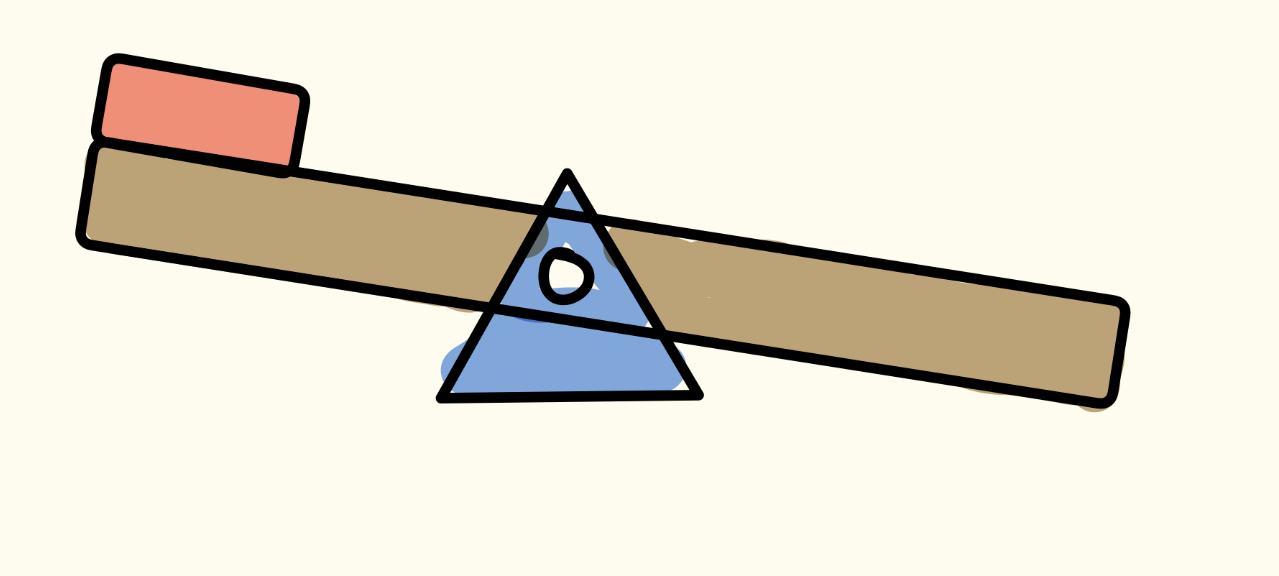
\includegraphics[width=0.5\linewidth]{opstelling.jpeg}
    \caption{Opstelling}
    \label{fig:Opstelling}
\end{figure}

\section{Voorbereiding}
Voor het experiment zijn de volgende onderdelen gebruikt:
\begin{itemize}
    \item \textbf{hefboom}, deze bestaat uit een houten plank met een as daardoorheen
    \item \textbf{multimeter voor stroom}, deze is in serie geschakeld met de batterij.
    \item{\textbf{multimeter voor spanning}, deze is in parallel geschakeld met de batterij en de \textit{load}.
    \item \textbf{\textit{load}}, deze zal bestaan uit een kleine elektromotor, om ervoor te zorgen dat het circuit de stroom ergens kwijt kan.
    \item \textbf{stopwatch} om een constante frequencie aan te houden tijdens de metingen.
\end{itemize}
In Figuur \ref{fig:Circuit} is een schema van de opstelling te zien en in Figuur \ref{fig:fysiek} de daadwerkelijke opstelling.
\begin{figure}[htbp]
    \centering
    \begin{minipage}{0.45\textwidth}
        \centering
        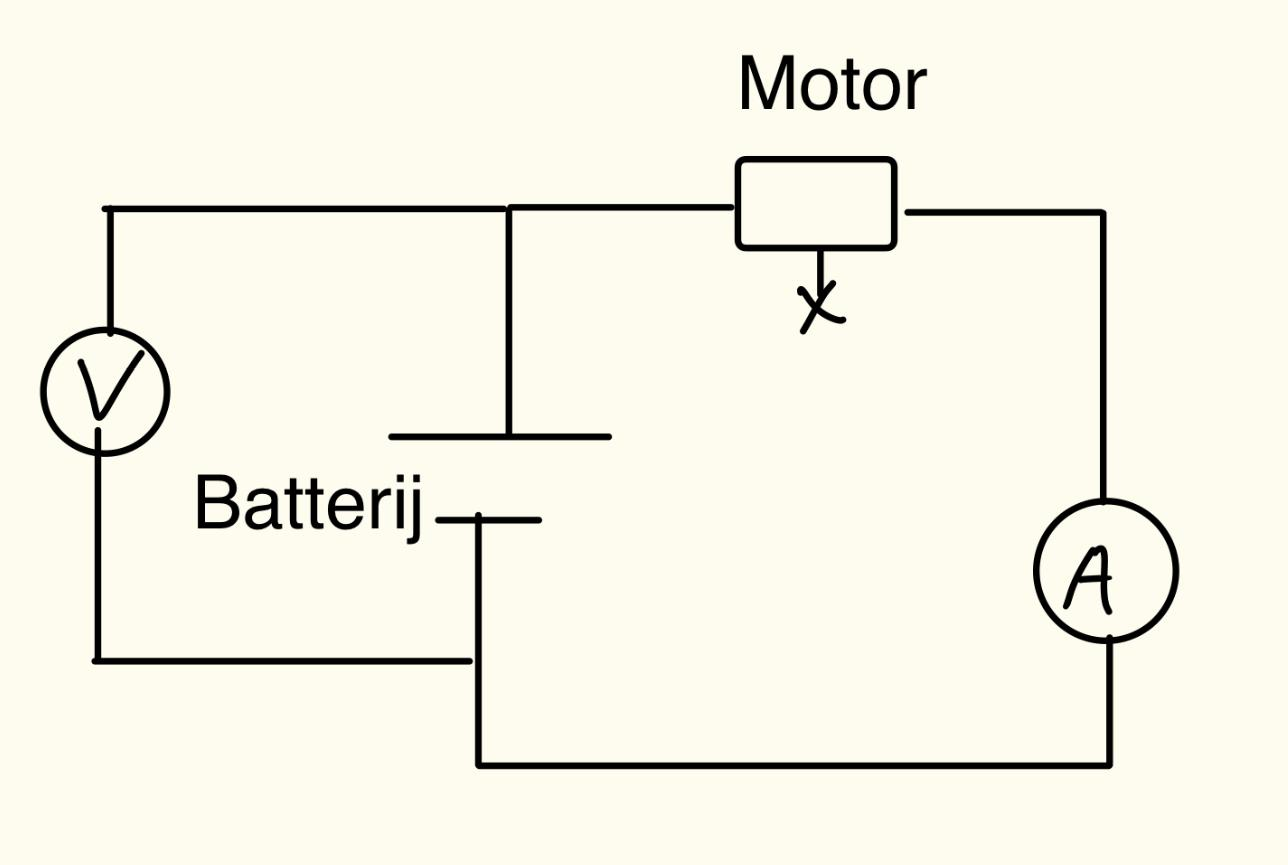
\includegraphics[width=\linewidth]{Circuit.jpeg}
        \caption{Circuit}
        \label{fig:Circuit}
    \end{minipage}\hfill
    \begin{minipage}{0.45\textwidth}
        \centering
        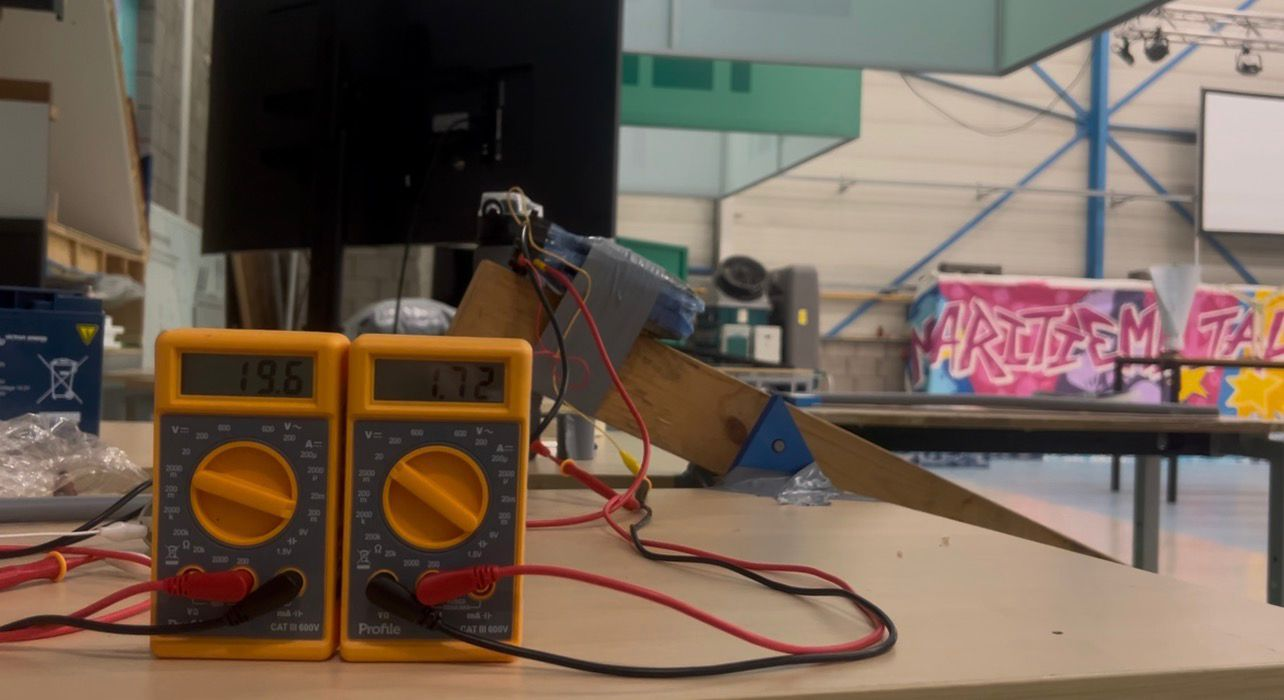
\includegraphics[width=\linewidth]{opstelling].jpeg}
        \caption{Opstelling fysiek}
        \label{fig:fysiek}
    \end{minipage}
\end{figure}

\section{Resultaten}
Met het experiment is de volgende data gerealiseerd:

\begin{table}[htbp]
\centering
\caption{Gemiddelde resultaten onderzoek }
\label{tab:experimental_results}
\begin{tabular}{l c S[table-format=2.3] S[table-format=1.3]}
\toprule
\textbf{Scenario} & \textbf{datapunten} & {\textbf{gemiddelde P (mW)}} & {\textbf{Std afwijking (mW)}} \\
\midrule
*Grote golven      & 60          & 33.664                 & 0.203                     \\
*Kleine golven     & 60          & 33.657                 & 0.172                     \\
\textbf{Statisch 0$^\circ$ (null)} & 60 & \textbf{33.398}     & \textbf{0.197}            \\
Statisch 45$^\circ$ & 59          & 33.442                 & 0.333                     \\
Statisch 90$^\circ$ & 60          & 33.164                 & 0.124                     \\
\bottomrule
\end{tabular}
\end{table}
*Bij de golf scenarios werd een frequentie van circa een trilling per seconde gebruikt, bij lichte golven een hoek van circa 20 graden en bij grote golven circa 45 graden.
\noindent
Deze tabel is een gemiddelde op basis van 60 datapunten met een tijdstap van een seconde, de volledige tabbellen zijn de te vinden in de bijlage [\ref{tab:static_0deg_data}].\\

\noindent
Het vermogen laat een lichte fluctuatie zien, deze fluctuatie is maximaal 0.8 procent van de nulmeting. Te observeren is dat de power afneemt van boven naar beneden in de tabel (bovenste meting is ook de eerste meting en de onderste de laatste meting), de hypothese hiervoor is dat de batterij iets leger is en daardoor (iets) minder krachtig is. 

\section{Conclusie}
Uit bovenstaande resultaten blijkt dat het verschil minder dan een procent is, in absolute termen 0.00026W. Hieruit wordt de conclusie getrokken dat golfbewegingen geen dan wel een verwaarloosbare invloed hebben op de praktische werking van de
batterij in de maritieme omgeving.

\section{Evaluatie}
Om de theorie te valideren dat de batterij leeg raakt en daardoor vermkogen verlies is, zou een volgend experiment gedaan moeten worden waar de batterij tussen sessies door naar het zelfde laadniveau gebracht moeten worden.
\chapter{Eindontwerp}
In dit hoofdstuk wordt onderzocht hoe de bevindingen vanuit dit rapport geimplementeerd kunnen worden voor Jansje.\\

\section{Eisen}
Voor een praktische implementatie zijn de volgende eisen belangrijk:
\begin{enumerate}
    \item Ruimte is niet essentieel voor eigenaar
    \item Beschermt tegen regen
    \item Voldoet aan brandveiligheidseisen
    \item Bereikbaar voor onderhoud
    \item Minimale GM van >0.15 volgens IMO-eisen \cite{IMO_A749}
  
\end{enumerate}\\


De batterijen thermisch geisoleerd zijn van de warmtebronnen (moto/uitlaat).\\
Bereikbaar voor onderhoud; hiermee wordt bedoeld dat een monteur de ruimte in moet kunnen en de batterijkabels aan de voor- en achterkant goed moet kunnen zien of daar makkelijk voor moet kunnen zorgen.\\
Water bij een elektrisch systeem is ongewenst voor de veiligheid door kortsluiting en slijtage.\\
Lage GM betekent dat de batterijen niet te hoog moeten zijn om het schip instabiel te maken.
\section{Beschikbare ruimtes}
Het schip kan in vijf ruimtes opgedeeld worden hier beneden schematisch weergegeven, de rode lijnen in figuur \ref{fig:Bovenkant} zijn de loop paden, de blauwe strepen geven aan op welke pekken van het dek daadwerkelijk nuttige ruime is.
\begin{figure}
    \centering
    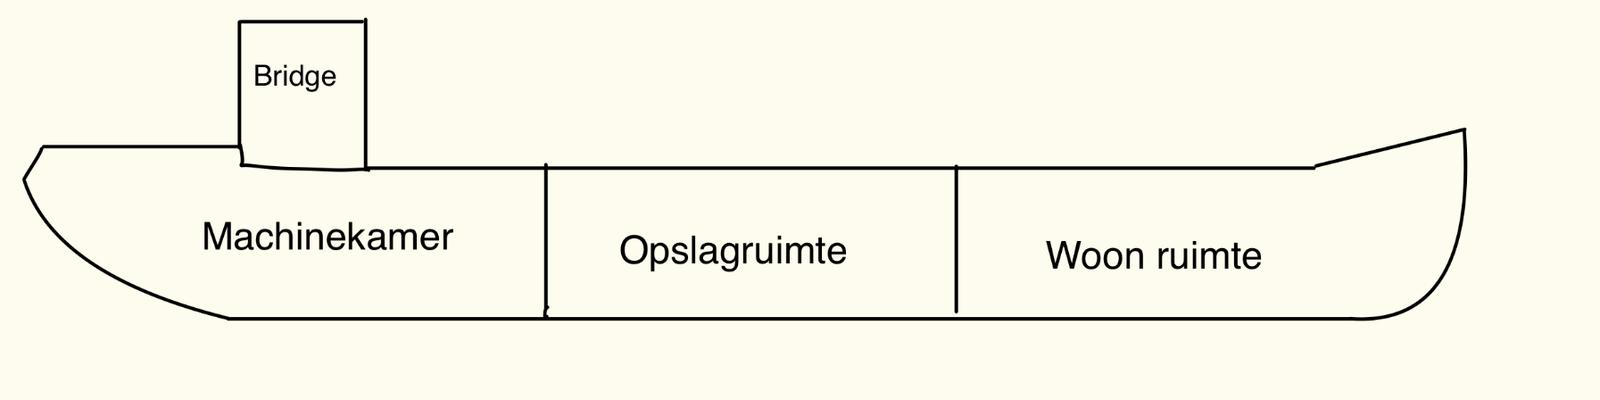
\includegraphics[width=0.8\linewidth]{vanaf de zijkant.jpeg}
    \caption{Zijprofiel van ruimtes}
    \label{fig:zijkant}
\end{figure}
\begin{figure}
    \centering
    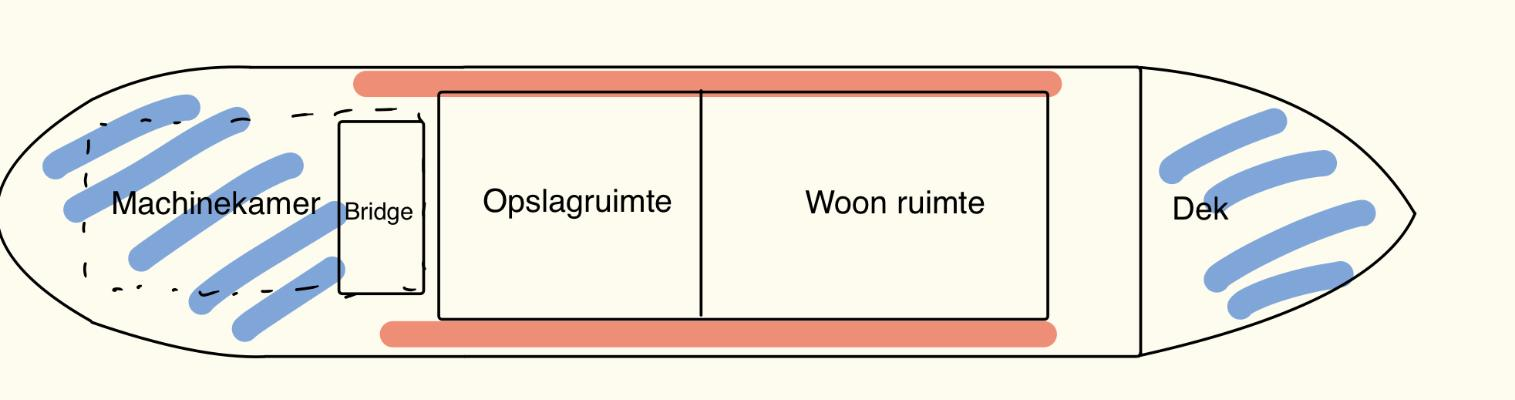
\includegraphics[width=0.8\linewidth]{vanaf boven.jpeg}
    \caption{Bovenprofiel van ruimtes}
    \label{fig:Bovenkant}
\end{figure}
\newpage
Nu worden de ruimtes getoetst aan de eerder gestelde eisen.\\
\\
De Bridge- en Woonruimte zijn essentieel voor de eigenaar en vallen af (eis 1).\\
Het dek is niet geschikt omdat deze niet tegen regen beschermt (eis 2).\\
Volgens ES-TRIN 2025 10.11 3 \cite{cesni2025inlandstandards} voldoet de machinekamer niet aan  brandveiligheidsseisen eis(3).\\
Alle ruimtes kunnen zo ingericht worden zodat ze bereikbaar zijn voor onderhoud (eis 4).\\
Omdat de bridge en het dek op het oppervlak van het schip zijn is de KG hoog (eis 5).\\
Dit wordt gevisualiseerd in de volgende matrix:

\begin{table}[htbp]
\centering
\caption{Evaluatie van scheepsruimtes op basis van functionele eisen}
\label{tab:ruimte_evaluatie}
\begin{tabular}{p{5cm}ccccc}
\toprule
\textbf{Functionele eis} & \textbf{Machinekamer} & \textbf{Opslagruimte} & \textbf{Woonruimte} & \textbf{Dek} & \textbf{Bridge} \\
\midrule
1. Ruimte is niet essentieel voor eigenaar & \cmark & \cmark & $\times$   & \cmark & $\times$   \\
\addlinespace
2. Beschermt tegen regen                   & \checkmark & \checkmark & \checkmark & $\times$   & \checkmark \\
\addlinespace
3. Voldoet aan brandveiligheidseisen       & $\times$   & \checkmark & \checkmark & \checkmark & \checkmark \\
\addlinespace
4. Bereikbaar voor onderhoud               & \checkmark & \checkmark & \checkmark & \checkmark & \checkmark \\
\addlinespace
5. Lage GM (Zwaartepunt)                   & \checkmark & \checkmark & \checkmark & $\times$   & $\times$   \\
\bottomrule
\end{tabular}
\end{table}
Dit geeft de volgende schematische weergave:
\begin{figure}[H]
    \centering
    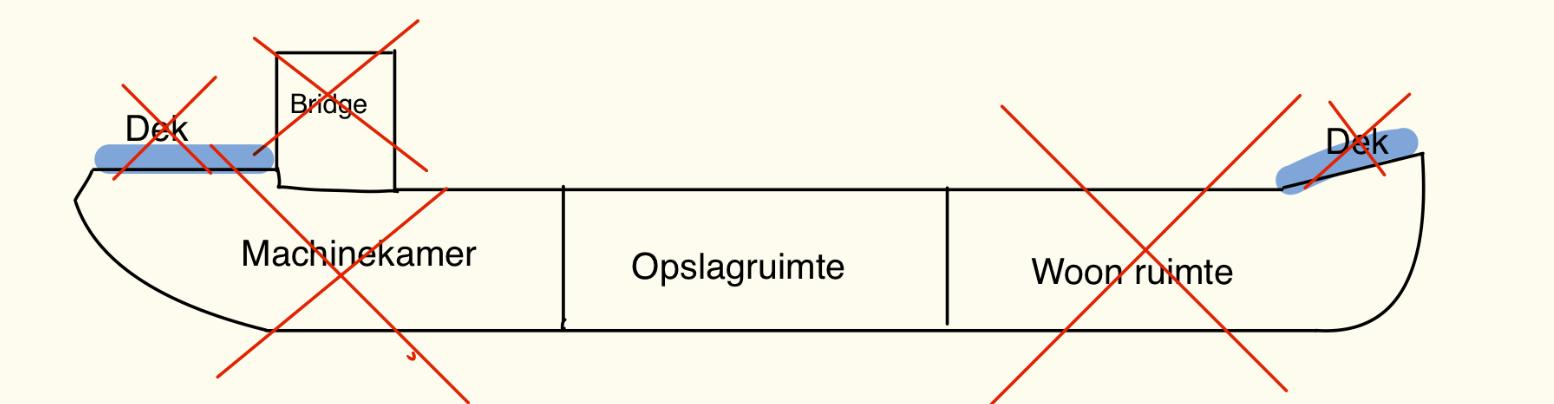
\includegraphics[width=0.8\linewidth]{afvallers.jpeg}
    \caption{Afvallers}
    \label{fig:Afvallers}
\end{figure}
Oftewel alleen de opslagruimte is als enige een optie voor de opslag van batterijen.
\newpage
\section{Inrichting opslagruimte}
Alhoewel alleen de opslagruimte een optie is, zijn er verschillende manieren om deze in te richten. Deze inrichtingen hebben invloed op eis 3, 4 en 5 en dus afgewogen om zo tot de beste inrichting te komen.\\
Voor eis 3 is er gekeken naar de richtlijnen die de Deense Maritieme Autoriteit heeft opgesteld, gevolgd. Deze worden gezien als de basis voor de toekomstige internationale regelgeving \cite{DMA_battery_operation_ships}.
\begin{itemize}
    \item De batterijruimte zal vrij zijn van hittebronnen en beschermd zijn tegen externe hitte door middel van hittebestendige isolatie.
    \item Er moet geschikt blusmateriaal aanwezig zijn voor een elektrische brand.
\end{itemize}\\

Voor eis 4 is er geen harde eis op een bepaalde afstand, het belangrijkst is dat de inspecteur/monteur door een bepaald looppad kan lopen om voor de batterij te komen de breedte van dit pad is ongeveer 0.6 meter \cite{Loopadbreedte}. Ook moet vanaf boven 0.2m speling zijn voor bedrading en dergelijken. Na gesprekken met dr. Ten wordt aangeraden dat de voorkant van de batterij bereikbaar is.\\
\\
Voor eis 5 wordt een minimale $GM$-waarde van $0{,}15$~m gehanteerd. Dit staat ook in het IMO-minimum voor dwarsscheepse stabiliteit \cite{IMO_A749}.
Zoals aangetoond in hoofdstuk~\ref{sec:stab_berekening} voldoen alle 
ontwerpen aan dit criterium.
\\


Voor het varen op nominaal vermogen is een vermogen nodig van 11 KW. De zeezoutbatterijen beter zijn op basis van de criteria ten opzichte van lithium batterijen. Om toch zoveel mogelijk gebruik te maken van zeezoutbatterijen is gewenst dat deze minimaal het nominale vermogen van 11KW kunnen leveren. Voor het optrekken van 22KW zouden dan LFP batterijen toegevoegd worden. Om dit te realiseren hebben is er een serie aandrijving nodig zoals weergegeven in figuur \ref{fig:Aandrijving}, hierbij kan de zeezout batterij eventueel bij bijvoorbeeld het afremmen de LFP batterijen op te laden om deze in de gewenste batterijpercentage window te houden.
\\
\begin{figure}[H]
    \centering
    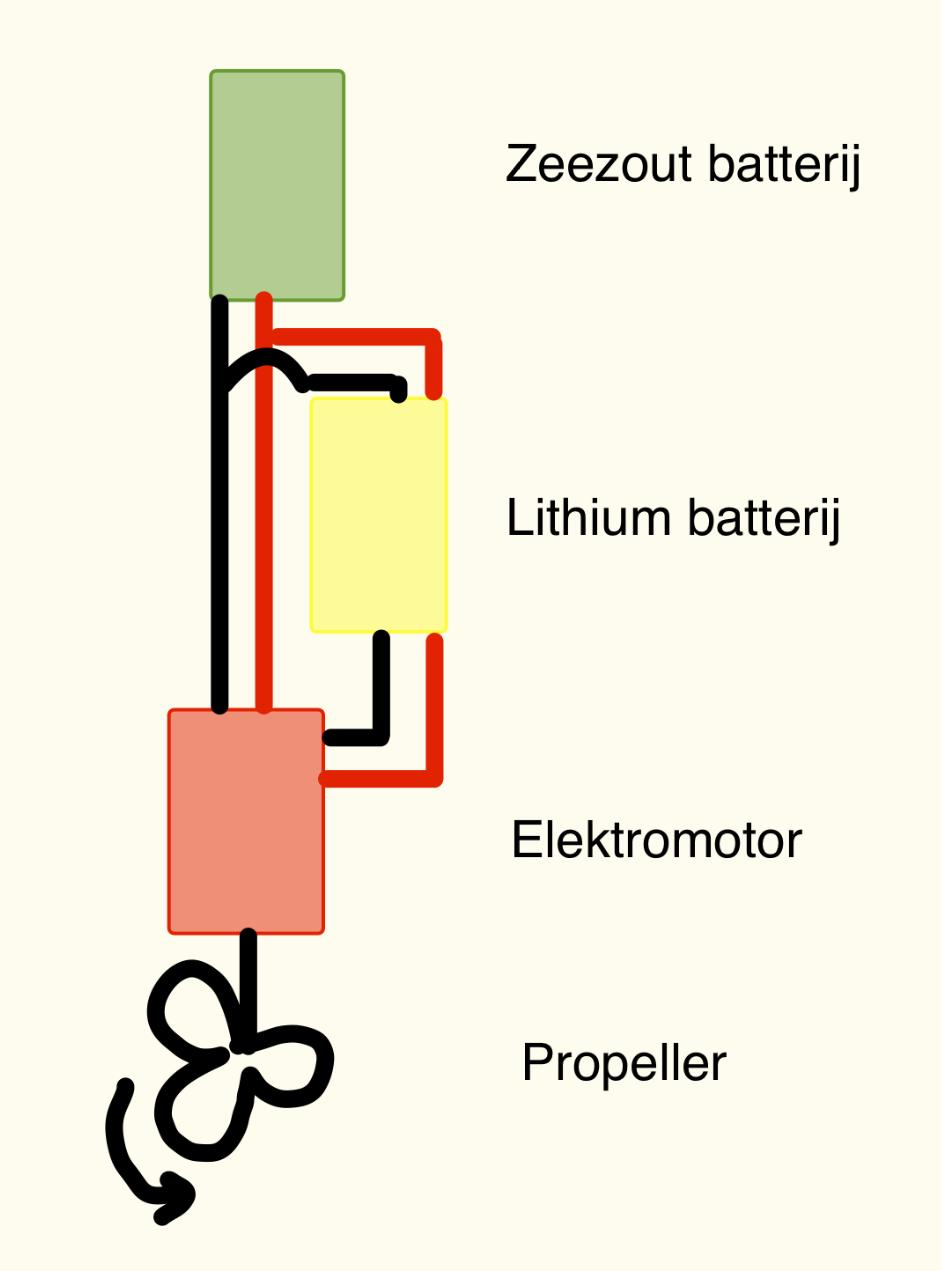
\includegraphics[width=0.5\linewidth]{aandrijving.jpeg}
    \caption{Serie aandrijving}
    \label{fig:Aandrijving}
\end{figure}
\\
\newpage
\paragraph{Zeezout}
\begin{equation*}
n_z = \left\lceil \frac{P_{\min,z}}{P_z} \right\rceil_5
    = \left\lceil \frac{10{,}8}{0{,}187} \right\rceil_5
    = \lceil 57{,}75 \rceil_5 = 60,
\qquad
E_z^{\text{lev}} = 60 \times 0{,}48 = 28{,}80\ \text{kWh}.
\end{equation*}

\paragraph{LFP (80\% operating window).}
\begin{equation*}
E_l^{\text{bruik}} = 0{,}80 \times 5{,}8 = 4{,}64\ \text{kWh},
\qquad
n_l = \left\lceil \frac{11{,}7}{5{,}9} \right\rceil_5 = \lceil 1{,}98 \rceil_5 = 5,
\qquad
E_l^{\text{lev}} = 5 \times 4{,}64 = 23{,}20\ \text{kWh}.
\end{equation*}

\paragraph{Capacity gap.}
\begin{equation*}
\Delta E = E_{\text{nodig}} - \bigl(E_z^{\text{lev}} + E_l^{\text{lev}}\bigr)
         = 108{,}15 - (28{,}80 + 23{,}20)
         = \boxed{56{,}15\ \text{kWh}}.
\end{equation*}

\\
Uit de berekening blijkt dat er ongeveer 60 zeezoutbatterijen toegevoegd moeten worden en ongeveer 5 LFP batterijen . De capaciteit van deze twee bij elkaar is totaal 52 kWh; er is totaal 108,15 kWh nodig, wat een capaciteitstekort van 56,15 KWh geeft. Deze kun je opvullen op verschillende manieren die verder worden uitgelicht in de ontwerpen.
\\
De ruimte is totaal 2.5x3x2 meter, oftewel 12 kubieke meter beschikbaar, waarbij lithiumbatterijen een hogere dichtheid hebben dan zeezoutbatterijen.
\\

Met het bovenstaande in gedachte kunnen drie ontwerpen afgewogen worden tegen elkaar.

\subsection{Ontwerp 1; zo duurzaam mogelijk }
Voor ontwerp 1 worden zoveel mogelijk zeezoutbatterijen toegevoegd en zo min mogelijk lithiumbatterijen.  De zeezoutbatterijen kunnen maximaal zeven hoog gestapelt worden en de LFP maximaal zes hoog, om te voldoen aan de voorwaardes en 2 meter hoog.

\begin{figure}[H]
    \centering
    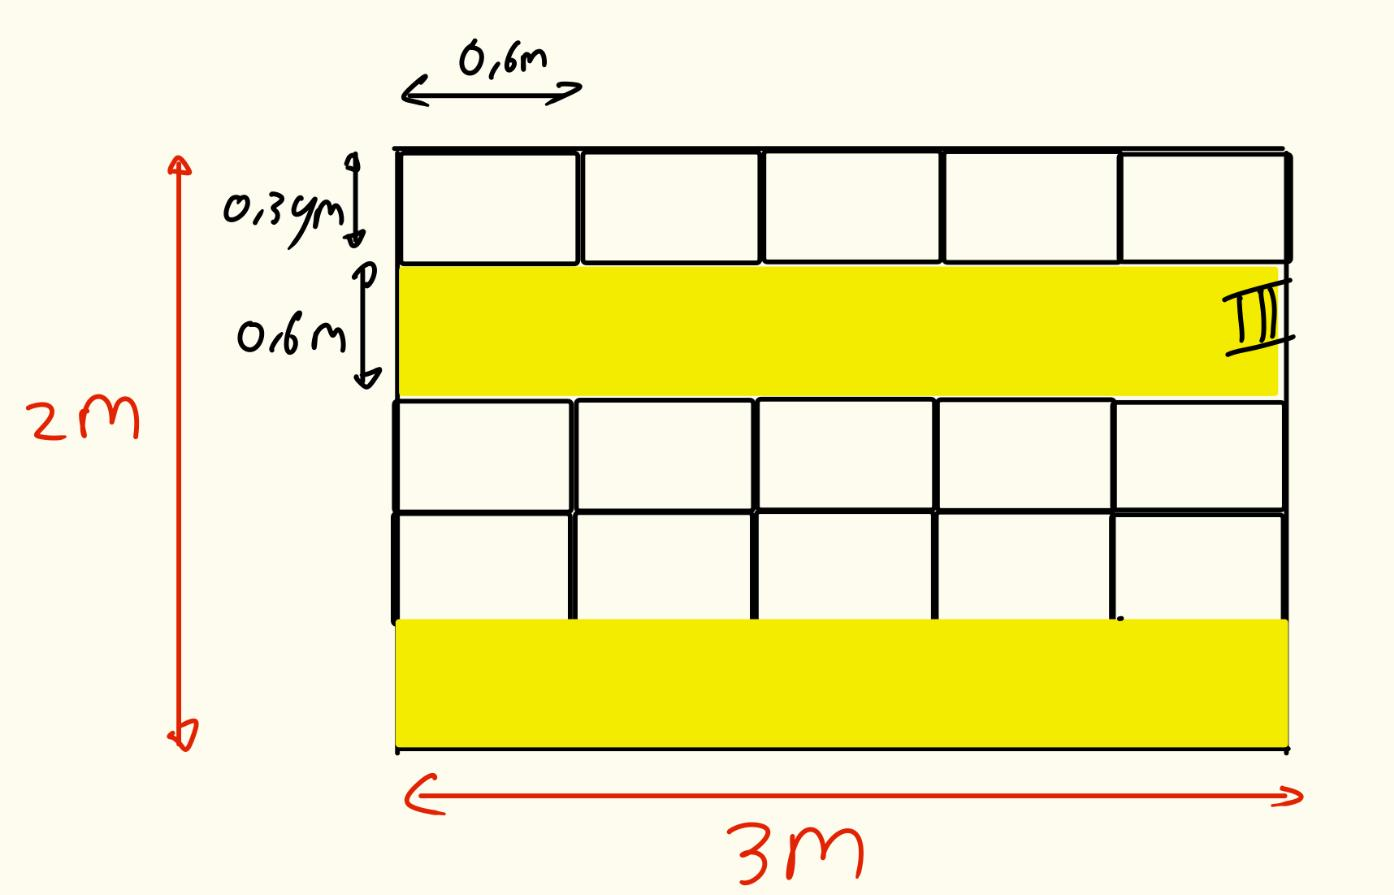
\includegraphics[width=0.5\linewidth]{inrichting alleen zeezout.jpeg}
    \caption{Initieele inrichting 1}
    \label{fig:Ontwerp 1}
\end{figure}\\

Op het figuur \ref{fig:Ontwerp 1} zijn 15 stapels mogelijk ofwel 105 batterijen. berekening, 50.4 KWh en 19.6 KW.
Elke stapel van zeezoutbatterijen die wordt vervangen door lithium voegt 29.12 KWh toe en 29.68 KW. Oftewel er moeten twee volle stapels van zeezout uit en twee volle stapels van lithium in om te voldoen aan de capiciteit van 108.15 KWh.
\begin{figure}[H]
    \centering
    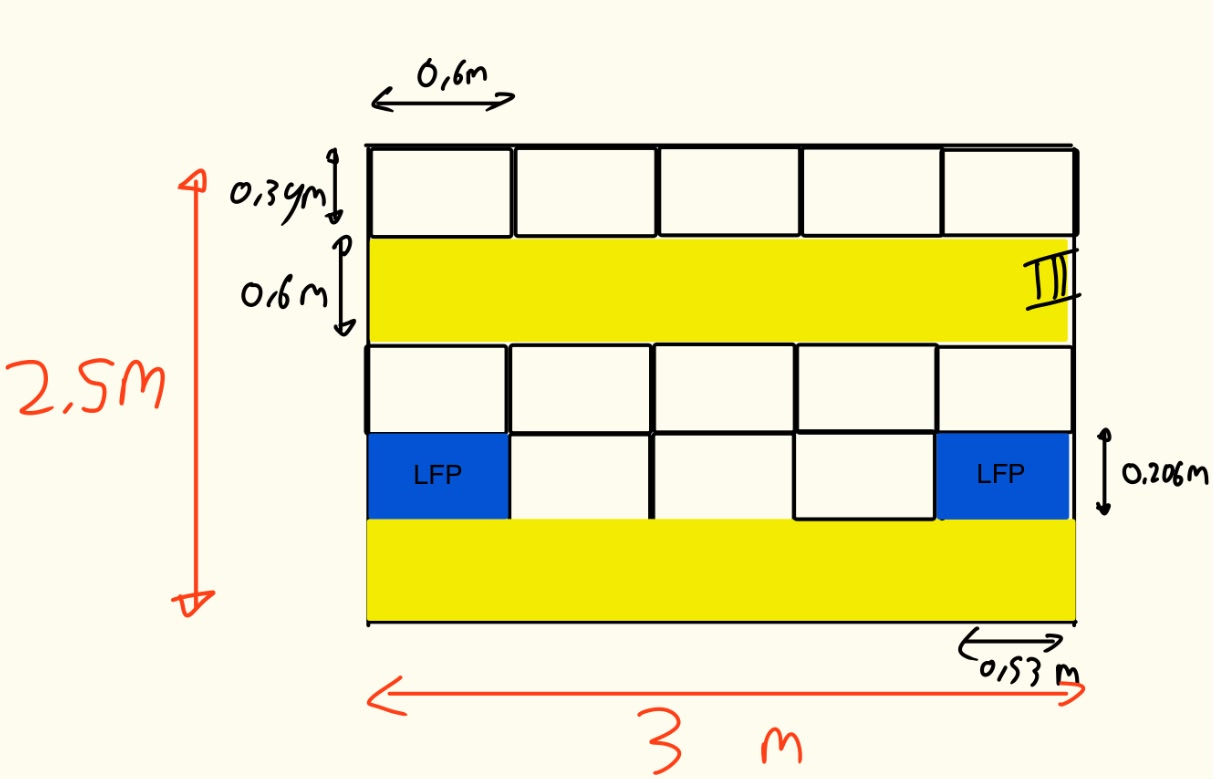
\includegraphics[width=0.5\linewidth]{setup A.jpeg}
    \caption{Ontwerp 1, blauw lithium, wit zeezout}
    \label{fig:Ontwerp 1}
\end{figure}\\
Bill of materials:\\
90 zeezoutbatterijen 88\%
12 LFP 12\%
102 totaal 100\%
\subsection{Ontwerp 2; zo goedkoop mogelijk}
Voor ontwerp 2 is het belangrijk dat de zeezoutbatterijen het nominale vermogen nog kunnen leveren, de rest wordt opgevangen door de LFP batterijen. Zoals eerder berekend \ref{} moeten er 60 zeezoutbatterijen en 18 lithiumbatterijen komen. Er is ruimte voor 16 stapels, de lithium batterij is het zwaarst dus die moet zo laag mogelijk zijn. Lithium worden 5 stapels totaal waarvan 3, 4 batterijen hoog zijn en de andere 2 stapels 3 batterijen hoog. Dan worden zeezoutbatterijen over 10 stapels allemaal van 6 hoog.
\begin{figure}[H]
    \centering
    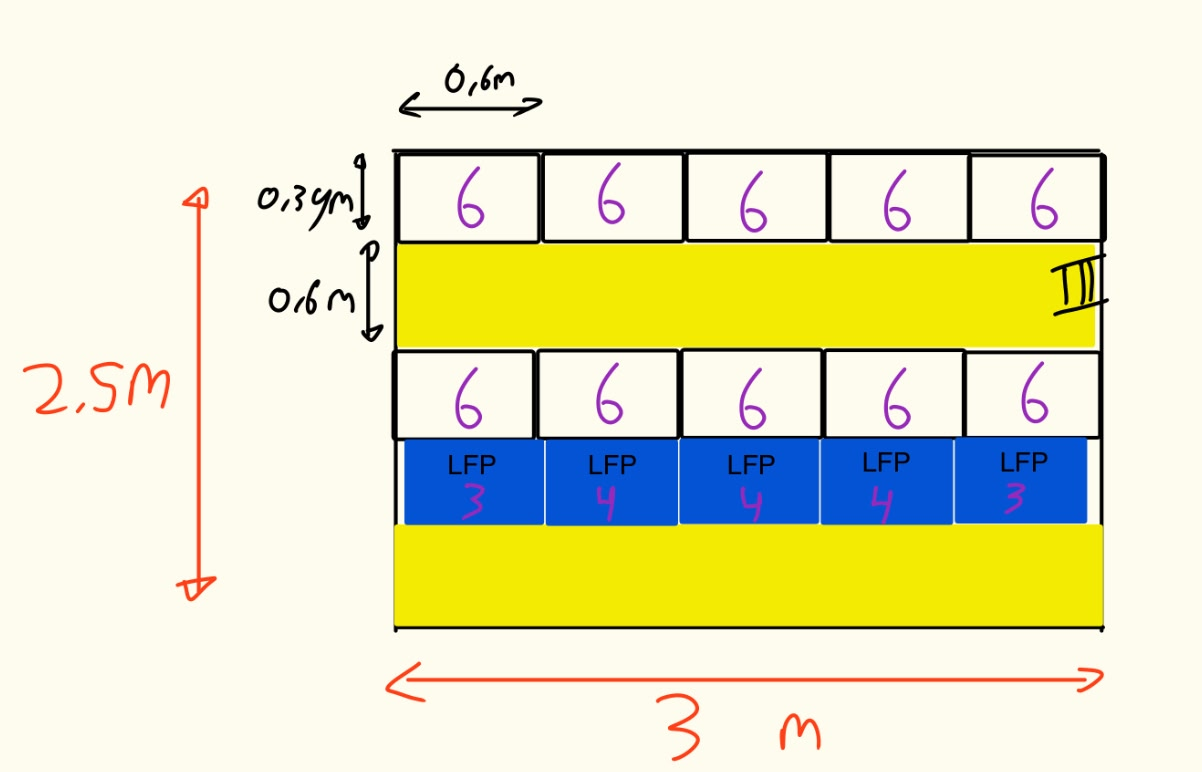
\includegraphics[width=0.6\linewidth]{design B.jpeg}
    \caption{Ontwerp 2, blauw lithium, wit zeezout}
    \label{fig:Ontwerp 1}
\end{figure}\\

Bill of materials:\\
90 zeezoutbatterijen 88\%
12 LFP 12\%
102 totaal 100\%
\subsection{Ontwerp 3; hybride van ontwerp 1 en ontwerp 2}
In ontwerp 1 en 2 is te zien dat er 15 stapels te maken zijn, waarvan tenminste 10 zeezout en 2 LFP moeten zijn. De overige 3 stapels kan zelf een combinatie voor gekozen worden, dat is design 3. Dit om een hybride combinatie tussen ontwerp 1 en 2 ook door te kunnen rekenen in de onderstaande gewogen criteria tabel.
\begin{figure}[H]
    \centering
    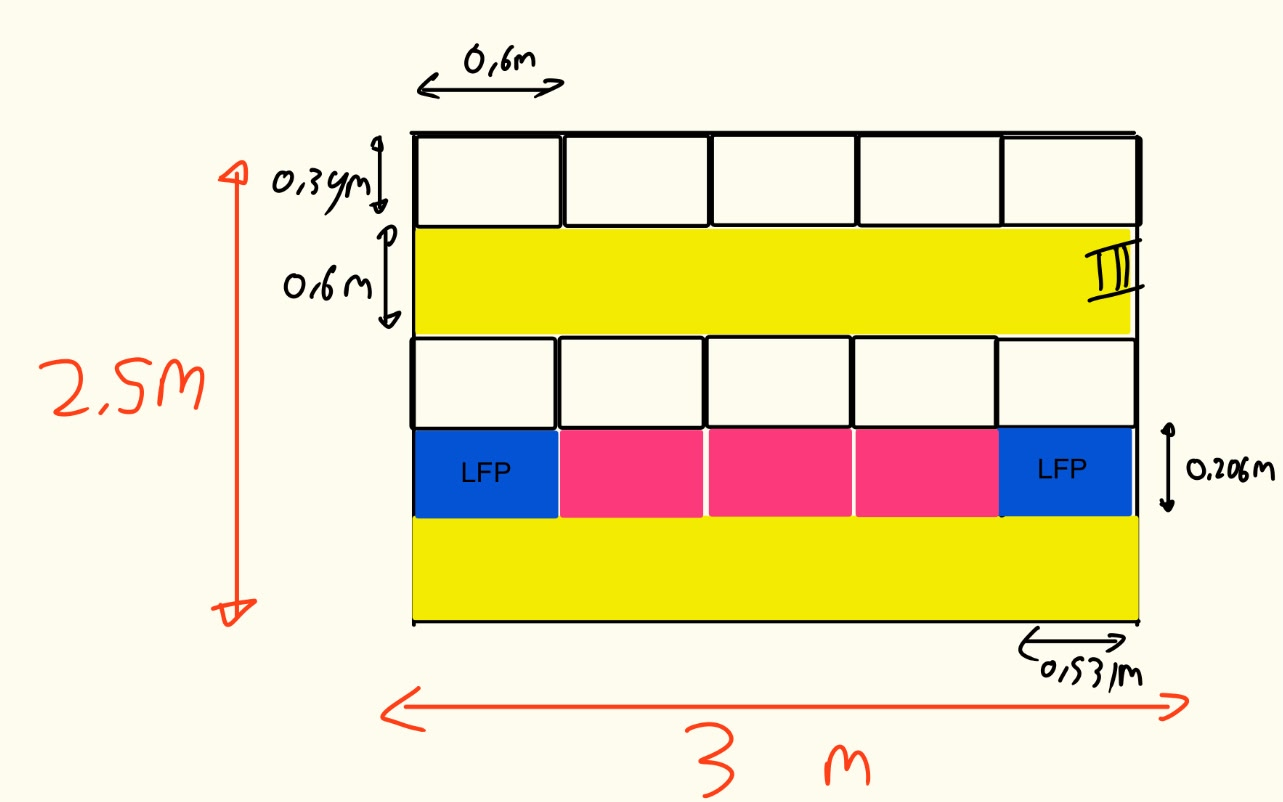
\includegraphics[width=0.6\linewidth]{Design C.jpeg}
    \caption{Ontwerp 3, waarbij roze zeezout of lfp kan zijn}
    \label{fig:Ontwerp 3}
\end{figure}\\

\subsection{Gewogen criteria tabel}
De designs worden afgewogen tegen elkaar, een groot deel van deze criteria  komen uit de gewogen criteria tabel van energieopslag [\ref{tab:allesheetdit}].\\
Omdat alle designs nominaal op zeezoutbatterijen kunnen varen, is de innovativiteit overal gelijk.

\begin{table}[H]
\centering
\caption{Scoretabel van energieopslagmethoden specifiek voor Jansje (genormaliseerde bronscores)}
\resizebox{\textwidth}{!}{
\begin{tabular}{lcccc}
\toprule
Criterium & Weging (\%) & Ontwerp 1 & Ontwerp 2 & Ontwerp 3\\
\midrule
Duurzaamheid                       & 16 & 4.87 & 4.76 & x \\
Innovativiteit                     & 15 & 4.74 & 4.50 & x \\
Kosten per effectieve kWh (€/kWh)  & 13 & 4.98 & 4.95 & x \\
Veiligheid                         & 13 & 4.87 & 4.75 & x \\
Levensduur (jaren)                 & 13 & 4.64 & 4.31 & x \\
CAPEX (€)                          & 12 & 1.50 & 1.94 & x \\
Efficiëntie (\%)                   & 10 & 4.99 & 4.98 & x \\
Massa (kg)                         &  8 & 1.63 & 2.10 & x \\
Totaal                             & 100 & 4.17 & 4.09 & x \\
\bottomrule
\end{tabular}
}
\label{tab:inrichting}
\end{table}

De scores zijn gebasseerd op de scores uit de gewogencriteria tabel voor energieopslag [\ref{tab:allesheetdit}], hierbij is gekeken naar de score van de batterij en het percentage van hoeveel deze voorkomt.\\
Bijvoorbeeld voor ontwerp 1: 88 procent van de batterijen is zeezoutbatterijen, de score in de tabel is 5.0 dus 0.88 x 5 = 4.4, LFP scoorde 3.94 dus 0.12 x 3.94 = 0.47, de totale score voor duurzaamheid wordt dan 4.87.
\begin{table}[h]
\centering
\caption{Scoretabel van energieopslagmethoden specifiek voor Jansje}
\resizebox{\textwidth}{!}{
\begin{tabular}{lcccccc}
\toprule
Criterium & Weging (\%) & LFP & Zeezoutbatterij (gen 4.0)\\
\midrule
Duurzaamheid                      & 16  & 3.94 & 5.00 \\
Innovativiteit                    & 15  & 2.83 & 5.00 \\
Kosten per effectieve kWh (€/kWh) & 13  & 4.80 & 5.00 \\
Veiligheid                        & 13  & 3.95 & 5.00 \\
Levensduur (jaren)                & 13  & 2.00 & 5.00 \\
CAPEX (€)                         & 12  & 5.00 & 1.02 \\
Efficiëntie (\%)                  & 10  & 4.90 & 5.00 \\
Massa (kg)                        &  8  & 5.00 & 1.19 \\
Totaal                            & 100 & 3.94 & 4.22 \\
\bottomrule
\end{tabular}
}
\label{tab:allesheetdit}
\end{table}

\section{CAD}
\begin{figure}[H]
    \centering
    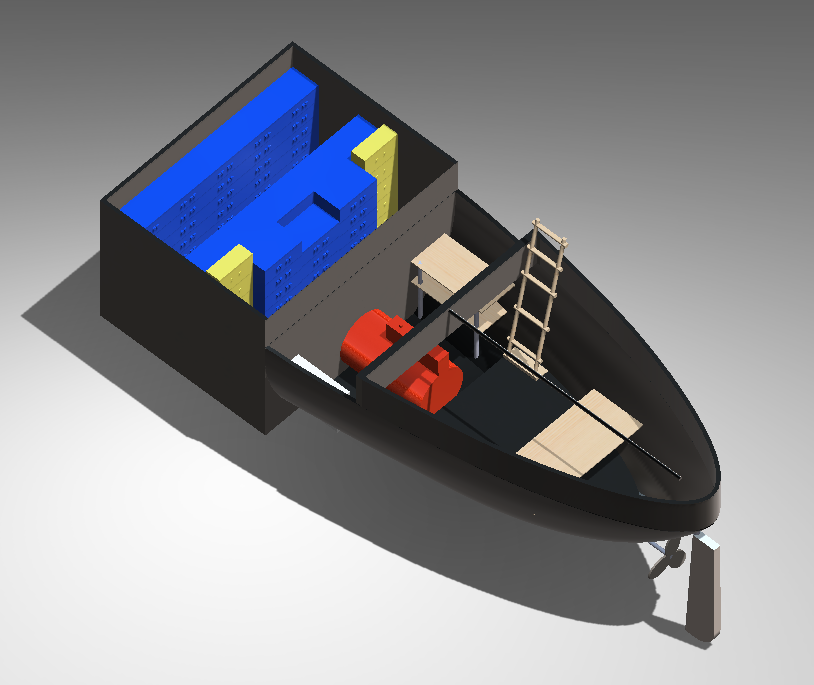
\includegraphics[width=0.9\linewidth]{Hoofdstukken/CAD.png}
    \caption{Ontwerp 1, blauw lithium, wit zeezout}
    \label{fig:Ontwerp 1}
\end{figure}\\
\section{Stabiliteitsberekening per ontwerp}
\label{sec:stab_ontwerpen}

Voor elk van de drie inrichtingsontwerpen is de dwarsscheepse stabiliteit
bepaald. De metacentrische hoogte $GM$ dient te voldoen aan het IMO-minimum
\cite[p.~44]{Barras2006}:

\begin{equation}
    GM = KB + BM - KG \geq 0{,}15\ \mathrm{m}
    \label{eq:GM_ontwerpen}
\end{equation}

De scheepsgeometrie en stabiliteitparameters voor de lege conditie
($KB_\mathrm{leeg} = 0{,}803$~m, $BM_\mathrm{leeg} = 1{,}384$~m,
$KG_\mathrm{leeg} = 1{,}30$~m) zijn voor alle ontwerpen gelijk aan de
waarden uit Hoofdstuk~\ref{chap:stabiliteit}. Alleen de ladingmassa
en het zwaartepunt van de lading verschillen per ontwerp.

% ----------------------------------------------------------
\subsection{Samenstelling en zwaartepuntschatting lading}
\label{sec:stab_samenstelling}

De drie ontwerpen onderscheiden zich in de verhouding zeezoutbatterijen en
LFP-modules. Een zeezoutcel ($18{,}7$~kg, $0{,}60 \times 0{,}39 \times
0{,}23$~m) is lichter dan een LFP-module ($40{,}0$~kg, $0{,}531 \times
0{,}206 \times 0{,}295$~m). Om het zwaartepunt van de lading zo laag
mogelijk te houden, worden de zwaardere LFP-modules altijd als onderste laag
geplaatst.

Het zwaartepunt van de lading $z_\mathrm{lad}$ is de hoogte boven de kiel.
Op basis van de scheepstekening \cite{JansjeTekening2026} bedraagt de
ruimbodem $\approx 0{,}30$~m boven kiel. De LFP-modules (hoogte $0{,}295$~m)
hebben daarmee een zwaartepunt op $0{,}30 + 0{,}148 \approx 0{,}45$~m boven
kiel. De zeezoutcellen worden daarboven gestapeld; het gemiddelde midden van
de stapel ligt op $0{,}30 + 1{,}00 = 1{,}30$~m boven kiel. Het gewogen
gemiddelde $z_\mathrm{lad}$ per ontwerp volgt uit:

\begin{equation}
    z_\mathrm{lad} =
    \frac{n_\mathrm{LFP} \cdot m_\mathrm{LFP} \cdot z_\mathrm{LFP}
        + n_z \cdot m_z \cdot z_z}
         {n_\mathrm{LFP} \cdot m_\mathrm{LFP} + n_z \cdot m_z}
    \label{eq:z_lad}
\end{equation}

\begin{table}[H]
\centering
\caption{Batterijsamenstelling en zwaartepuntschatting lading per ontwerp.
         Alle hoogten zijn gemeten boven de kiel \cite{JansjeTekening2026}.}
\label{tab:samenstelling}
\begin{tabular}{lcccccc}
\toprule
Ontwerp & $n_z$ & $n_\mathrm{LFP}$
        & $M_\mathrm{lad}$ [t]
        & $z_z$ [m] & $z_\mathrm{LFP}$ [m] & $z_\mathrm{lad}$ [m] \\
\midrule
1 -- zo duurzaam mogelijk & 91 & 12 & 2{,}18 & 1{,}30 & 0{,}45 & 1{,}24 \\
2 -- zo goedkoop mogelijk & 60 & 18 & 1{,}84 & 1{,}30 & 0{,}45 & 1{,}04 \\
3 -- hybride              & 70 & 14 & 1{,}87 & 1{,}30 & 0{,}45 & 1{,}14 \\
\bottomrule
\end{tabular}
\vspace{4pt}

\noindent\footnotesize
\textit{%
$n_z$: aantal zeezoutcellen ($m_z = 18{,}7$~kg);
$n_\mathrm{LFP}$: aantal LFP-modules ($m_\mathrm{LFP} = 40{,}0$~kg).
$z_z = 1{,}30$~m: zwaartepunt zeezoutcellen boven kiel
(ruimbodem $0{,}30$~m $+$ gemiddeld halve stapelhoogte $\approx 1{,}00$~m).
$z_\mathrm{LFP} = 0{,}45$~m: zwaartepunt LFP-modules boven kiel
(ruimbodem $0{,}30$~m $+$ halve modulehoogte $0{,}148$~m).
Ruimbodemhoogte afgeleid uit scheepstekening \cite{JansjeTekening2026}.}
\end{table}

% ----------------------------------------------------------
\subsection{Rekenmodel}
\label{sec:stab_rekenmodel}

De stabiliteitparameters in geladen conditie worden als volgt bepaald:

\begin{align}
    T_\mathrm{gel}  &= T_\mathrm{leeg} + \frac{M_\mathrm{lad}}{A_{WP}}
    \label{eq:T_gel} \\[4pt]
    KB_\mathrm{gel} &= 0{,}535 \times T_\mathrm{gel}
    \label{eq:KB_gel} \\[4pt]
    BM_\mathrm{gel} &= \frac{I_T}{\nabla_\mathrm{gel}}
                     = \frac{101{,}1}{\nabla_\mathrm{leeg} + M_\mathrm{lad}}
    \label{eq:BM_gel} \\[4pt]
    KG_\mathrm{gel} &= \frac{W \cdot KG_\mathrm{leeg}
                            + M_\mathrm{lad} \cdot z_\mathrm{lad}}
                            {W + M_\mathrm{lad}}
    \label{eq:KG_gel} \\[4pt]
    GM_\mathrm{gel} &= KB_\mathrm{gel} + BM_\mathrm{gel} - KG_\mathrm{gel}
    \label{eq:GM_gel}
\end{align}

met $A_{WP} = 77{,}0\ \mathrm{m^2}$, $\nabla_\mathrm{leeg} = 73{,}0\ \mathrm{m^3}$
en $W = 73{,}0\ \mathrm{t}$.

% ----------------------------------------------------------
\subsection{Ontwerp 1 -- zo duurzaam mogelijk}
\label{sec:stab_ontwerp1}

Ontwerp~1 bevat 91~zeezoutcellen en 12~LFP-modules
($M_1 = 2{,}18$~t, $z_\mathrm{lad,1} = 1{,}24$~m).

\begin{align}
    T_{\mathrm{gel},1}      &= 1{,}500 + \tfrac{2{,}18}{77{,}0}
                             = 1{,}528\ \mathrm{m}
                             \quad(\text{vrijboord} = 0{,}522\ \mathrm{m}) \\[4pt]
    \nabla_{\mathrm{gel},1} &= 73{,}0 + 2{,}18 = 75{,}2\ \mathrm{m^3} \\[4pt]
    KB_{\mathrm{gel},1}     &= 0{,}535 \times 1{,}528 = 0{,}817\ \mathrm{m} \\[4pt]
    BM_{\mathrm{gel},1}     &= \tfrac{101{,}1}{75{,}2} = 1{,}345\ \mathrm{m} \\[4pt]
    KG_{\mathrm{gel},1}     &= \frac{73{,}0 \times 1{,}30 + 2{,}18 \times 1{,}24}
                                    {75{,}2}
                             = \frac{94{,}90 + 2{,}70}{75{,}2}
                             = 1{,}298\ \mathrm{m} \\[6pt]
    \Aboxed{GM_{\mathrm{gel},1}} &\Aboxed{= 0{,}817 + 1{,}345 - 1{,}298
                             = 0{,}864\ \mathrm{m}}
\end{align}

% ----------------------------------------------------------
\subsection{Ontwerp 2 -- zo goedkoop mogelijk}
\label{sec:stab_ontwerp2}

Ontwerp~2 bevat 60~zeezoutcellen en 18~LFP-modules
($M_2 = 1{,}84$~t, $z_\mathrm{lad,2} = 1{,}04$~m). De relatief grote
fractie zware LFP-modules onderaan geeft het laagste ladingszwaartepunt
van de drie ontwerpen.

\begin{align}
    T_{\mathrm{gel},2}      &= 1{,}500 + \tfrac{1{,}84}{77{,}0}
                             = 1{,}524\ \mathrm{m}
                             \quad(\text{vrijboord} = 0{,}526\ \mathrm{m}) \\[4pt]
    \nabla_{\mathrm{gel},2} &= 73{,}0 + 1{,}84 = 74{,}8\ \mathrm{m^3} \\[4pt]
    KB_{\mathrm{gel},2}     &= 0{,}535 \times 1{,}524 = 0{,}815\ \mathrm{m} \\[4pt]
    BM_{\mathrm{gel},2}     &= \tfrac{101{,}1}{74{,}8} = 1{,}352\ \mathrm{m} \\[4pt]
    KG_{\mathrm{gel},2}     &= \frac{73{,}0 \times 1{,}30 + 1{,}84 \times 1{,}04}
                                    {74{,}8}
                             = \frac{94{,}90 + 1{,}91}{74{,}8}
                             = 1{,}294\ \mathrm{m} \\[6pt]
    \Aboxed{GM_{\mathrm{gel},2}} &\Aboxed{= 0{,}815 + 1{,}352 - 1{,}294
                             = 0{,}873\ \mathrm{m}}
\end{align}

% ----------------------------------------------------------
\subsection{Ontwerp 3 -- hybride}
\label{sec:stab_ontwerp3}

Ontwerp~3 bevat 70~zeezoutcellen en 14~LFP-modules
($M_3 = 1{,}87$~t, $z_\mathrm{lad,3} = 1{,}14$~m).

\begin{align}
    T_{\mathrm{gel},3}      &= 1{,}500 + \tfrac{1{,}87}{77{,}0}
                             = 1{,}524\ \mathrm{m}
                             \quad(\text{vrijboord} = 0{,}526\ \mathrm{m}) \\[4pt]
    \nabla_{\mathrm{gel},3} &= 73{,}0 + 1{,}87 = 74{,}9\ \mathrm{m^3} \\[4pt]
    KB_{\mathrm{gel},3}     &= 0{,}535 \times 1{,}524 = 0{,}815\ \mathrm{m} \\[4pt]
    BM_{\mathrm{gel},3}     &= \tfrac{101{,}1}{74{,}9} = 1{,}350\ \mathrm{m} \\[4pt]
    KG_{\mathrm{gel},3}     &= \frac{73{,}0 \times 1{,}30 + 1{,}87 \times 1{,}14}
                                    {74{,}9}
                             = \frac{94{,}90 + 2{,}13}{74{,}9}
                             = 1{,}294\ \mathrm{m} \\[6pt]
    \Aboxed{GM_{\mathrm{gel},3}} &\Aboxed{= 0{,}815 + 1{,}350 - 1{,}294
                             = 0{,}871\ \mathrm{m}}
\end{align}

% ----------------------------------------------------------
\subsection{Vergelijkingstabel}
\label{sec:stab_vergelijk}

\begin{table}[H]
\centering
\caption{Stabiliteitscomponenten per ontwerp -- geladen conditie}
\label{tab:stab_vergelijk}
\begin{tabular}{lrrrrl}
\toprule
Grootheid & Leeg & Ontwerp 1 & Ontwerp 2 & Ontwerp 3 & Eenheid \\
\midrule
\multicolumn{6}{l}{\textit{Lading}} \\[2pt]
Zeezoutcellen $n_z$          &  --     &  91     &  60     &  70     & --    \\
LFP-modules $n_\mathrm{LFP}$ &  --     &  12     &  18     &  14     & --    \\
Ladingmassa $M_\mathrm{lad}$ &  --     & 2{,}18  & 1{,}84  & 1{,}87  & t     \\
\midrule
\multicolumn{6}{l}{\textit{Drijfvermogen}} \\[2pt]
Diepgang $T$                 & 1{,}500 & 1{,}528 & 1{,}524 & 1{,}524 & m     \\
Vrijboord                    & 0{,}550 & 0{,}522 & 0{,}526 & 0{,}526 & m     \\
$\nabla$                     & 73{,}0  & 75{,}2  & 74{,}8  & 74{,}9  & m$^3$ \\
\midrule
\multicolumn{6}{l}{\textit{Stabiliteitscomponenten}} \\[2pt]
$KB$                         & 0{,}803 & 0{,}817 & 0{,}815 & 0{,}815 & m \\
$BM$                         & 1{,}384 & 1{,}345 & 1{,}352 & 1{,}350 & m \\
$KG$                         & 1{,}300 & 1{,}298 & 1{,}294 & 1{,}294 & m \\
\midrule
\rowcolor{green!15}
$GM$ & \textbf{0{,}887} & \textbf{0{,}864}
     & \textbf{0{,}873} & \textbf{0{,}871} & m \\
\midrule
\multicolumn{6}{l}{\textit{Toetsing}} \\[2pt]
IMO-min.\ $GM \geq 0{,}15$~m \cite[p.~44]{Barras2006}
  & \checkmark & \checkmark & \checkmark & \checkmark & -- \\
Vrijboord $\geq 0{,}20$~m
  & \checkmark & \checkmark & \checkmark & \checkmark & -- \\
\bottomrule
\end{tabular}
\end{table}

% ----------------------------------------------------------
\subsection{Grafische vergelijking}
\label{sec:stab_grafiek}

\begin{figure}[H]
\centering
\begin{tikzpicture}
\begin{axis}[
    ybar,
    bar width        = 22pt,
    width            = 0.78\textwidth,
    height           = 8.5cm,
    enlarge x limits = 0.20,
    symbolic x coords= {Leeg,{Ontwerp 1},{Ontwerp 2},{Ontwerp 3}},
    xtick            = data,
    xticklabel style = {font=\small},
    ylabel           = {$GM$ [m]},
    ymin             = 0,
    ymax             = 1.10,
    % Nette ytick-waarden zonder overlap met de stippellijn-labels
    ytick            = {0, 0.2, 0.4, 0.6, 0.8, 1.0},
    yticklabel style = {/pgf/number format/fixed,
                        /pgf/number format/precision=1,
                        font=\small},
    nodes near coords,
    nodes near coords align = {above},
    every node near coord/.append style = {font=\small},
    grid             = major,
    grid style       = {dashed, gray!35},
    % Legenda linksbovenin zodat die niet overlapt met balken
    legend style     = {at={(0.03,0.97)}, anchor=north west, font=\small},
    title            = {Metacentrische hoogte $GM$ per ontwerp (geladen conditie)},
    title style      = {font=\small},
    clip             = false,   % zodat node buiten plotgebied kan staan
]

%% Blauwe balken
\addplot[fill=blue!55, draw=blue!75!black]
    coordinates {
        (Leeg,        0.887)
        ({Ontwerp 1}, 0.864)
        ({Ontwerp 2}, 0.873)
        ({Ontwerp 3}, 0.871)
    };
\addlegendentry{$GM_\mathrm{gel}$}

%% IMO-minimum -- één doorlopende lijn van links naar rechts
\addplot[
    thick, red!80!black, dashed, forget plot
] coordinates {(Leeg, 0.15) ({Ontwerp 3}, 0.15)};

%% IMO-label: boven de lijn, vlak bij de rechteras, buiten de laatste balk
\node[
    red!80!black, font=\small, anchor=south east
] at (axis cs:{Ontwerp 3}, 0.15) {IMO-min.\ $0{,}15$~m \quad};

\end{axis}
\end{tikzpicture}
\caption{$GM$ in geladen conditie voor de lege toestand en de drie
         batterijontwerpen. De gestippelde rode lijn geeft het IMO-minimum
         van $0{,}15$~m weer \cite[p.~44]{Barras2006}. Alle ontwerpen
         voldoen ruimschoots. Ruimbodemhoogte gebaseerd op scheepstekening
         \cite{JansjeTekening2026}.}
\label{fig:GM_vergelijk}
\end{figure}

% ----------------------------------------------------------
\subsection{Conclusie}
\label{sec:stab_conclusie_ontwerpen}

Alle drie de ontwerpen voldoen ruimschoots aan het IMO-minimum van
$0{,}15$~m. De metacentrische hoogte in geladen conditie ligt voor elk
ontwerp in het bereik $0{,}864$--$0{,}873$~m. Het onderlinge verschil
tussen de ontwerpen bedraagt maximaal $0{,}009$~m en is daarmee
verwaarloosbaar. De stabiliteit vormt voor geen van de ontwerpen een
beperkende factor bij de ontwerpselectie.


\subsection{Ontwerpkeuze?}

Nu de keuze is gemaakt voor ontwerp 1 moet worden onderzocht of het systeem voldoet aan de eisen. In het systeem zijn 91 zeezoutbatterijen en 12 LFP-batterijen. Echter is de capaciteit die met deze hoeveelheid batterijen bereikt wordt meer dan de eerder gestelde randvoorwaarde van 108.15 kWh \ref{}, namelijk 113.28 \ref{}. Daarom kan er in theorie worden bespaard op de hoeveelheid zeezoutbatterijen. Deze hebben een lagere capaciteit dan de LFP-batterij (0.48 kWh tegenover 5.8 kWh) waardoor enkel met minder zeezoutbatterijen nog voldaan kan worden aan de randvoorwaarde. Door negen zeezoutbatterijen minder mee te nemen is de capaciteit 108.96 kWh, hiermee wordt nog steeds voldaan aan de randvoorwaarde. 

\noindent Een schip dat vaart op elektrische batterijen kan gebruik maken van verschillende voltages, er zijn meerdere opties. Een laag voltage betekent dat de stroomsterkte door de kabels hoog is. Dit brengt bepaalde veiligheidsrisico's en complicaties met zich mee maar is wel erg efficiënt. Aan de andere kant betekent een hoog voltage dat de stroomsterkte lager is en de gebruiksgemak veiligheidrisico's hoger zijn. Zoals eerder benoemd zijn er 82 zeezoutbatterijen en 12 LFP-batterijen nodig. Beide batterijen leveren standaard 24 V \ref{}\ref{}, om een voltage van 48 V te bereiken moeten paren worden gemaakt van 


\begin{table}[h!]
\centering
\caption{Vergelijking van Batterijconfiguraties voor Het Jansje (Basis: 12 LFP en 90 Zeezout)}
\label{tab:batterij_vergelijking_compleet}
\begin{tabular}{|l||l|c|c|c|c|}
\hline
\textbf{Systeemspanning} & \textbf{Batterijtype} & \textbf{Schakeling} & \textbf{Max. Vermogen} & \textbf{Stroomsterkte} & \textbf{Totale Opslag} \\ 
 & & \textbf{(Serie / Parallel)} &  & & \\ \hline\hline

 & LFP  & $1\text{S} \times 12\text{P}$ & 70.68 kW & & 69.60 kWh \\ \cline{2-4} \cline{6-6}
\textbf{24 V} & Zeezout & $1\text{S} \times 90\text{P}$ & 16.83 kW & 916.7 A & 43.20 kWh \\ \cline{2-4} \cline{6-6}
 & \textbf{Totaal} & \textbf{--} & \textbf{87.51 kW} & & \textbf{112.80 kWh} \\ \hline\hline

 & LFP  & $2\text{S} \times 6\text{P}$ & 35.34 kW & & 69.60 kWh \\ \cline{2-4} \cline{6-6}
\textbf{48 V} & Zeezout & $2\text{S} \times 41\text{P}$ & 7.67 kW & 458.3 A & 39.36 kWh \\ \cline{2-4} \cline{6-6}
 & \textbf{Totaal} & \textbf{--} & \textbf{43.01 kW} & & \textbf{108.96 kWh} \\ \hline\hline

 & LFP  & $3\text{S} \times 4\text{P}$ & 23.56 kW & & 69.60 kWh \\ \cline{2-4} \cline{6-6}
\textbf{72 V} & Zeezout & $3\text{S} \times 30\text{P}$ & 5.61 kW & 305.6 A & 43.20 kWh \\ \cline{2-4} \cline{6-6}
 & \textbf{Totaal} & \textbf{--} & \textbf{29.17 kW} & & \textbf{112.80 kWh} \\ \hline\hline

 & LFP & $4\text{S} \times 3\text{P}$ & 17.67 kW & & 69.60 kWh \\ \cline{2-4} \cline{6-6}
\textbf{96 V} & Zeezout & $4\text{S} \times 20\text{P}$ & 3.74 kW & 229.2 A & 38.40 kWh \\ \cline{2-4} \cline{6-6}
 & \textbf{Totaal} & \textbf{--} & \textcolor{red}{21.41 kW} & & \textcolor{red}{108.00 kWh} \\ \hline\hline

 & LFP & $5\text{S} \times 2\text{P}$ & 11.78 kW & & 58.00 kWh \\ \cline{2-4} \cline{6-6}
\textbf{120 V} & Zeezout & $5\text{S} \times 18\text{P}$ & 3.37 kW & 183.3 A & 43.20 kWh \\ \cline{2-4} \cline{6-6}
 & \textbf{Totaal} & \textbf{--} & \textcolor{red}{15.15 kW} & & \textcolor{red}{101.20 kWh} \\ \hline\hline
\end{tabular}
\end{table}

Bij de oplossing met een voltage van 48 V worden maar 82 zeezoutbatterijen gebruikt, dit is precies de minimale hoeveelheid en dus kan de rest zo worden geschakeld dat deze dienen als reservevoorziening.
Deze overige negen kunnen worden gebruikt als reserve energievoorziening om te voldoen aan de veiligheidseis \ref{}. 







\chapter{Aandrijfsysteemkeuze}

\noindent Nu het energieopslagstysteem is bepaald, kan onderzocht worden wat de meeste geschikte aandrijving zal zijn. Dit is tevens deelvraag 3:
\begin{quote}
    \textit{\textbf{Welk aandrijfsysteem is het meest geschikt voor transportschip Jansje, rekening houdend met
het gekozen energieopslagsysteem en het programma van eisen?}}
\end{quote}
\noindent Het gekozen energieopslagsysteem is een combinatie van zeezoutbatterijen en LFP batterijen. Dit zorgt er in ieder geval voor dat de huidige dieselmotor zal moeten worden vervangen door een elektromotor, in het geval dat keuze op een bio-brandstof zou vallen zou deze nog kunnen worden omgebouwd en hergebruikt maar in deze configuratie is dat geen optie. In dit hoofdstuk zullen randvoorwaarden worden opgesteld waaraan de nieuwe elektromotor zal moeten voldoen. Vervolgens zullen verschillende elektromotoren worden vergeleken en zal de best mogelijke optie worden gekozen.

\subsection{Randvoorwaarden}
\begin{enumerate}
    \item Het minimale benodigde vermogen wat de elektromotor aan zal moeten kunnen, bedraagt 22 kW \ref{}.
    \item De schroef draait in het huidige systeem op 600 RPM \cite{mail arnold}, dit betekent dat de nieuwe motor op hetzelfde toerenaantal zal moeten draaien of dat er een overbrenging nodig is. 
    \item Bij een toerental van 600 RPM is een koppel van 350 Nm nodig zoals berekend in de bijlage \ref{eq:koppelberekening}
    \item Uit metingen die plaats hebben gevonden op het schip blijkt dat de beschikbare ruimte voor het aandrijfsysteem (lxbxh) 1.4 x 0.7 x 1.0 m is.     
    \item Het voltage van de elektromotor bedraagt 48 V \ref{}.
    \item Vanwege het feit dat het energieopslagsysteem van het schip een direct stroom levert (DC) \cite{} is het rekening houdend met de kosten handig om een DC- motor aan te schaffen. Echter is het met een conversiesysteem wel mogelijk om gebruik te maken van een AC- motor dus hoeft deze optie niet uitgesloten te worden. 
\end{enumerate}



\noindent 

\section{}
Als een motor aan de bovenstaande eisen voldoet, kan deze worden toegepast in Jansje. Er zijn veel verschillende motoren op de markt met geschikte eigenschappen die goed bij Jansje zouden kunnen passen. Daarom is er één voorbeeldmotor gekozen om onder andere de prijs te kunnen bepalen. Een andere motor die aan dezelfde eisen voldoet, zou in principe ook geschikt kunnen zijn.


\subsection{Voorbeeld motor}
Als voorbeeldmotor is gekozen voor de GM22.5 Elektromotor van Green Marine. Deze motor is geselecteerd omdat Green Marine een Nederlands bedrijf is en de motor daardoor goed aansluit bij de Nederlandse markt. De prijs kan daarom worden gebruikt als realistische indicatie voor vergelijkbare motoren die mogelijk geschikt zijn voor Jansje. Omdat de motor een nominaal toerental van 1200 rpm heeft en het gewenste schroefastoerental 600 rpm is, is een 2:1 reductieoverbrenging nodig.

\begin{table}[h]
    \centering
    \caption{Belangrijkste specificaties van de GM22.5 elektromotor}
    \label{tab:gm22-5-motor}
    \begin{tabular}{ll}
        \hline
        \textbf{Eigenschap} & \textbf{Waarde\cite{greenmarine_gm225_datasheet}} \\
        \hline
        Model & GM22.5 Elektromotor \\
        Motortype & 3-fase PMSM \\
        Prijs & Nog te bepalen via mailcontact \\
        Vermogen & 22.5 kW \\
        Accuspanning & 40--65 V, 48 V nominaal \\
        Maximaal koppel & 180 Nm \\
        Nominaal toerental & 1200 rpm \\
        IP-klasse & IP68 \\
        Gewicht motor & ca. 65 kg \\
        Minimale kabeldikte & 120 mm$^2$ \\
        \hline
    \end{tabular}
\end{table}

\chapter{Aanbevelingen}

\subsection{Brandveiligheidseisen} 
Voor de brandveiligheid moet aan een aantal dingen voldaan worden om in compliantie te zijn met de (toekomstige) brandveiligheidseisen voor batterijen op schepen. Omdat er nog geen internationale regelgeving is voor brandveiligheid bij batterijen op schepen, worden de richtlijnen die de Deense Maritieme Autoriteit heeft opgesteld, gevolgd. Deze worden gezien als de basis voor de toekomstige internationale regelgeving \cite{DMA_battery_operation_ships}. Echter, omdat deze regelgeving nog niet bestaat, is het mogelijk om met goed verstand een aantal van deze systemen later te implementeren, om zo de kosten enigszins te verspreiden.

In de richtlijnen staat het volgende:

\begin{itemize}
    \item De batterijen zullen in een aparte ruimte worden geplaatst.
    \item de batterijruimte zal vrij zijn van hittebronnen en beschermd zijn tegen externe hitte door middel van hittebestendige isolatie.
    \item de batterijruimte zal een actieve ventilatie hebben, 
    \item een geschikt, automatisch brandblussysteem zal aanwezig zijn, welke voldoet aan de door de batterijfabrikant gegeven specificaties.
\end{itemize}
\chapter{Bijlage}



\noindent Verantwoording wegingen

\begin{figure}[h]
    \centering
    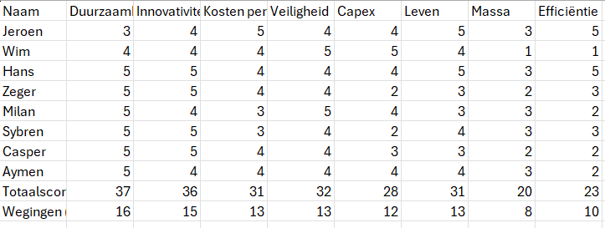
\includegraphics[width=0.5\linewidth]{tabel wegingen.png}
    \caption{Wegingen bepalen}
    \label{fig:wegingen}
\end{figure}

\subsection{Vergelijking van batterijen}
\begin{table}[h]
\centering
\caption{Vergelijking van batterijen \cite{Szewczyk2023}}
\begin{tabular}{lcccc}
\toprule
Batterijtype & Veiligheid & Kosten & Levensduur (cycli) & Energiedichtheid (Wh/kg) \\
\midrule
NMC & + & + & 1500 & 200 \\ 
LFP & ++ & + & 3000 & 120 \\ 
LTO & ++ & - - & 10000 & 80 \\
LCO & - - & + & 1000 & 200 \\
LMO & + & ++ & 700 & 150 \\
NCA & + & ++ & 500 & 260 \\
G-NMC & + & + & 8000 & 130 \\
\bottomrule
\end{tabular}
\label{tab:vergelijking_batterijen}
\end{table}


\begin{table}[h]
\centering
\caption{Vergelijking van energieopslagmethoden per eenheid}
\resizebox{\textwidth}{!}{
\begin{tabular}{lcccccc}
\toprule
Criterium & Weging (\%) & LFP & Zeezoutbatterij (gen 4.0) &  Waterstof (druk)  \\
\midrule
CAPEX (€) & 10 & 2.468,00 &   &\\
OPEX (€) & 10 & 1.4 & Is toch zelfde als LFP? Gewoon stroom, vgm geen onderhoud & \\
Massa (kg) & 5 & 40 & 18.7  & 1\\
Energiedichtheid/gewicht (Wh/kg) & -- &  145  & 25.89  & &\\
Energiedichtheid/volume (Wh/dm$^3$) & -- &180& 34.05  & \\
Efficiëntie (\%) & 10 & \approx 92 &97  & \\
Innovativiteit (\%) & 10 & 2.6 & 4.6 & 4.0 \\
Duurzaamheid (Score) & - & 3.94 & 5.00 & 3.72 & \\
Veiligheid  &  & 3.4 & 4.3 & 2.0 \\
\bottomrule
\end{tabular}
}
\label{tab:prestatievergelijking_uitgebreid}
\end{table}




\begin{table}[h]
\centering
\caption{Berekeningen van energieopslagmethoden per eenheid WORDT BIJLAGE}
\resizebox{\textwidth}{!}{
\begin{tabular}{lcccccc}
\toprule
Criterium & Weging (\%) & LFP & Zeezoutbatterij (gen 4.0) & Zeezoutbatterij (gen 6.0) & Waterstof (druk) \\
\midrule
CAPEX (€) & 10 & 2.468,00\cite{mg_price_list_2026}  &  & &\\
OPEX (€) & 10 & 0.24€/kWh \times 5.8 kWh \approx 1.4 \cite{mg_lfp_datasheets_page_2026}\cite{independer2026stroomprijs} & & &\\
Massa (kg) & 5 & 40 \cite{mg_lfp_datasheets_page_2026} &  Massa 1 cel is 146 g (0.4-2.0V), in elke batterij zitten 128 cellen, dus batterij (24 V, 20 Ah) weegt 18.7 kg & 1 & 1\\
Energiedichtheid/gewicht (Wh/kg) & -- & $\frac{5800Wh}{40kg}$ = 145 \cite{mg_lfp_datasheets_page_2026} & Gebaseerd op gravimetrische energiedichtheid (25.89 Wh/kg) & &\\
Energiedichtheid/volume (Wh/dm$^3$) & -- & $\frac{5800Wh}{2.95 dm \cdot 5.31 dm \cdot 2.06 dm}$ = 180 \cite{mg_lfp_datasheets_page_2026}& 34.05 & &\\
Efficiëntie (\%) & 10 & \approx 92 \cite{redondoiglesias2022efficiency}& 97& &\\
Innovativiteit (\%) & 10 & 2.6 & 4.6 &4.6 & 4.0 \\
Duurzaamheid (?) &  & &  & & \\
Veiligheid (1/5)  &  & 3.4 & 4.3 &  4.3 & 2.0 \\
\bottomrule

\end{tabular}
}
\label{tab:prestatievergelijking_uitgebreids}
\end{table}

\subsection{Opladen van zeezoutbatterij}

Tijdens het opladen is de volgende data gerealiseert:
\subsubsection{Setup}
For voltage measurement a multimeter is used.\\
For current measurement the gauge of the powersource is used.\\
Power source is an old (car)batterycharger. Can charge at 6V and 12V. We initialy set the power source to 6V.\\
surrounding temperature: 13degrees (outside temp, buienalarm, 17-5-26, 12:00, Baambrugge). battery is near an open window.\\
a test load (DC motor) is occacionaly used to determine if the load can be used for the actual test, and to read of the current with the multimeter, as it's probably more accurate than the gauge on the old charger.\\
During the experiment, at 11:54, two cables with small diameter are added to the circuits, to lower the charging current.

\subsubsection{\textbf{SSB charging log}}
start: 11:30
charge voltage:2.93v
charge current: 3.5A
\\\\
11:31: current keeps rising, now at 4 A\\
11:32: power shutoff, discharge current: 3.2A. discharge voltage 1.75\\
11:33: resume charging, 4A at 2.91V.\\
11:33: load checked, works.\\
11:35: heat check: no warmth discharge from the battery.\\
11:38: attempt to switch power source from 6V to 12V, current immediately rises to 6A (which is the max reading of the current gauge, so maybe more?). Actual voltage rises to 3.56.\\
11:38: switched back to 6V power source, so now charging at 2.87V, but current stays at 6+ A.\\
11:40: heat check of power soucre: slight warmth radiating from power source.\\
11:40: power source shut-off, attempt to let the load cycle. Battery doesn't yet have enough current. discharge power at steady 1.75V.\\
11:45: charging voltage has risen to 2.99V.\\
11:49: charging stopped. Power source is rated for 4A constant charging, where the battery continuously charged at 6+ A, for which the old power source wasn't designed.\\
11:49: heat check: no warmth discharge from battery. warmth discharge on power source slightly increased compared to previous measurement.\\
11:54: continue charging. Added some small cables inbetween to reduce charging current. Current is now at 2.4A, voltage at 4.04V.\\
11:55: power source makes small buzzing sound, probably also was there before, but didn't notice untill I checked.\\
11:55: tried to switch to 12V, current went to 4A, and voltage to 6.4V. However, as this is an old power source, charging at 4A continouusly will propbably damage it, so switched back to 6V.\\
11:57: charging at 4.17V, 2.2A.\\
11:58: voltage dropped to 3.85V, current still at 2.2A.\\
12:01: heat check: no warmth discharge from the battery, heat discharge from power source decreased. closed the window, it got cold and as the battery doesn't have any warmth discharge, no need for cooling.\\
12:01: voltage increased to 3.97V, current still 2.2A\\
12:03: voltage dropped to 3.89V, current 2.1A (current difference might be due to old equipment).\\
12:05: voltage increased to 3.91V, current 2.1A.\\
12:06: turned the multimeter upside down, then right side up, current now reads 4.01V.\\
12:12: steady charging at 4V, 2.1A. It also seems that the battery (4sacks in parallel, so 4 cells?) are rated for max 2.4A current, although the provided literature is a bit vague on what charging parameters to use. (is one sack one cell? And does "box of 4 blocks in parallel, 8 in series" mean box of 4 cells in parallel or 8 cells in series?\\
12:36: still charging at 4V, 2.1A.\\
12:36: heat check, seasalt battery has a very slight warmth, power source warmth decreased.\\
12:40: stopped charging, checked if battery can power load, which was succesfull.\\
12:42:'visual battery inspection. The leads of the cells seam to be rather soft, the clamps of the charger slightly deformed them.\\
12:45: amp test: output currently 0.27A.\\
12:52: resume normal charging. Due to slightly improves circuit, charging at 5.2V, 2.1A.\\
12:53: charged for approx 1hour, 0.27A.\\
13:03: charging at 5.3V,2.1A.\\
13:05 heat check: power source has negligible heat dissipation. Battery has slight heat dissipation, though only slightly sensible. Battery might have become a bit stiffer, although this has not been previously checked, and therefore can also not be the case. Small wires that where used start to heat up. might be wise to change them.\\
13:07: stop charging to swap out the small cables so they don't overheat.\\
13:08: discharge at 1.8V, which is quite good.\\
13:09: resumed charging, 5.4V at 2A. Swapped out the small cables for other ones of the same length, thickness, rating etc. old cables where cold already when I swapped them, and new ones where almost immediately the same temp as the old ones, so it seems to be just heat dissipation from the current, not accumulating heat, thus the cables do exactly what we want (act as additional resistance by dissipating heat). Connections of the multimeter have also improved, readings have become more stable.\\
13:41: steadily charging at 5.5V, 1.99A. slight local heat dissipation of the battery, though not even near concerning.\\
14:22: visual inspection: no notable differences.\\
14:22: heat inspection: heat dissipation from the battery increased more than previously measured. small cables are warm, but not concerning.\\
14:22: still charging at 5.5V, 2A. Even though the battery starts to warm up a bit, I would expect a drop in current when the battery is (almost) fully charged.\\
14:30: stopped charging.\\
14:30: voltage test: open circuit is 1.7V, closed circuit with load is 1.1V. Should the closed circuit lpad be 1.7V as well when fully charged?\\
14:33: resumed charging, 5.5V, 2A.\\
14:40: visual inspection: I noticed some hardened droplets on the top of the cells. They could just be adhesive used to seal the bags, but they might also be leakeage? Luckily, as this is a seasalt battery, there shouldn't be any harm to me.\\
14:45: stopped charging, ending the charging. The battery should be sufficiently charged for the upcomming test. \\
19:19: upon visual inspection: under certain light angle, slight yellow discoloration can be seen, although very slight. 


\subsubsection{\textbf{Looking back}}
The initial current of 6+ A at 3V is in line with the fact that the battery was deeply discharged. Also in line is the fact that, when the battery gains charge, the voltage increases and the current drops. According to the manufacturer, the charging time would be approximately eight hours. However, with three hours of charging, the battery should have enough charge for the experiment. Visualy inspecting the battery later, showed yellow coloring in the battery. According to the manufacturer this is due to crystals forming due to slight (local?) overcharging. however, In literature it is stated that a drop in charging current and rise in voltage should occur when the battery is near-full, which hasn't happened. This would lead to the conclusion that the battery might not have been optimaly functioning. However, this likely won't affect the experiment, as long as it keeps enough charge to complete the experiment.

\subsubsection{\textbf{For the future}}
The material of the poles are very soft, electrical clamps damage the surface and deform it. Furthermore, the poles aren't guarded, so putting them in a bag for traveling could create a current through the bag if the material is conducting. Therefore, for future experiments with similar cells I would advise to create a simple, hard plastic case and additional poles of a stronger metal.


\subsection{Volledige metingen experiment}
\begin{table}[htbp]
\centering
\caption{Volledige meetreeks voor de Hard Rocking conditie}
\label{tab:hard_rocking_data}
\begin{tabular}{c S[table-format=2.2] S[table-format=1.2] S[table-format=2.3]}
\toprule
\textbf{Meting (\#)} & {\textbf{Stroom I (mA)}} & {\textbf{Spanning V (V)}} & {\textbf{Vermogen P (mW)}} \\
\midrule
1  & 19.49 & 1.72 & 33.523 \\
2  & 19.93 & 1.72 & 34.280 \\
3  & 19.54 & 1.72 & 33.609 \\
4  & 19.61 & 1.72 & 33.729 \\
5  & 19.52 & 1.72 & 33.574 \\
6  & 19.56 & 1.73 & 33.839 \\
7  & 19.55 & 1.72 & 33.626 \\
8  & 19.58 & 1.72 & 33.678 \\
9  & 19.50 & 1.72 & 33.540 \\
10 & 19.46 & 1.72 & 33.471 \\
11 & 19.53 & 1.72 & 33.592 \\
12 & 19.51 & 1.72 & 33.557 \\
13 & 19.52 & 1.73 & 33.770 \\
14 & 19.58 & 1.73 & 33.873 \\
15 & 19.54 & 1.72 & 33.609 \\
16 & 19.57 & 1.72 & 33.660 \\
17 & 19.53 & 1.72 & 33.592 \\
18 & 19.51 & 1.72 & 33.557 \\
19 & 19.54 & 1.72 & 33.609 \\
20 & 19.50 & 1.72 & 33.540 \\
21 & 19.54 & 1.72 & 33.609 \\
22 & 19.62 & 1.72 & 33.746 \\
23 & 19.49 & 1.72 & 33.523 \\
24 & 19.46 & 1.73 & 33.666 \\
25 & 19.98 & 1.72 & 34.366 \\
26 & 19.48 & 1.72 & 33.506 \\
27 & 19.58 & 1.72 & 33.678 \\
28 & 19.52 & 1.72 & 33.574 \\
29 & 19.95 & 1.72 & 34.314 \\
30 & 19.53 & 1.72 & 33.592 \\
31 & 19.47 & 1.73 & 33.683 \\
32 & 19.42 & 1.73 & 33.597 \\
33 & 19.47 & 1.72 & 33.488 \\
34 & 19.56 & 1.72 & 33.643 \\
35 & 19.55 & 1.72 & 33.626 \\
36 & 19.56 & 1.72 & 33.643 \\
37 & 19.68 & 1.72 & 33.850 \\
38 & 19.54 & 1.72 & 33.609 \\
39 & 19.51 & 1.72 & 33.557 \\
40 & 19.65 & 1.72 & 33.798 \\
41 & 19.51 & 1.72 & 33.557 \\
42 & 19.47 & 1.72 & 33.488 \\
43 & 19.55 & 1.72 & 33.626 \\
44 & 19.48 & 1.72 & 33.506 \\
45 & 19.49 & 1.72 & 33.523 \\
46 & 19.56 & 1.72 & 33.643 \\
47 & 19.54 & 1.72 & 33.609 \\
48 & 19.48 & 1.72 & 33.506 \\
49 & 19.45 & 1.72 & 33.454 \\
50 & 19.48 & 1.73 & 33.700 \\
51 & 19.48 & 1.73 & 33.700 \\
52 & 19.58 & 1.73 & 33.873 \\
53 & 19.59 & 1.72 & 33.695 \\
54 & 19.96 & 1.72 & 34.331 \\
55 & 19.51 & 1.72 & 33.557 \\
56 & 19.52 & 1.72 & 33.574 \\
57 & 19.58 & 1.72 & 33.678 \\
58 & 19.49 & 1.72 & 33.523 \\
59 & 19.49 & 1.72 & 33.523 \\
60 & 19.48 & 1.72 & 33.506 \\
\bottomrule
\end{tabular}
\end{table}
\begin{table}[htbp]
\centering
\caption{Volledige meetreeks voor de Light Rocking conditie}
\label{tab:light_rocking_data}
\begin{tabular}{c S[table-format=2.2] S[table-format=1.2] S[table-format=2.3]}
\toprule
\textbf{Meting (\#)} & {\textbf{Stroom I (mA)}} & {\textbf{Spanning V (V)}} & {\textbf{Vermogen P (mW)}} \\
\midrule
1  & 19.60 & 1.72 & 33.712 \\
2  & 19.60 & 1.72 & 33.712 \\
3  & 19.60 & 1.72 & 33.712 \\
4  & 19.60 & 1.73 & 33.908 \\
5  & 19.60 & 1.72 & 33.712 \\
6  & 19.60 & 1.72 & 33.712 \\
7  & 19.60 & 1.73 & 33.908 \\
8  & 19.60 & 1.72 & 33.712 \\
9  & 19.50 & 1.73 & 33.735 \\
10 & 19.60 & 1.72 & 33.712 \\
11 & 19.50 & 1.72 & 33.540 \\
12 & 19.60 & 1.72 & 33.712 \\
13 & 19.60 & 1.72 & 33.712 \\
14 & 19.60 & 1.72 & 33.712 \\
15 & 19.60 & 1.72 & 33.712 \\
16 & 19.60 & 1.72 & 33.712 \\
17 & 19.50 & 1.72 & 33.540 \\
18 & 19.60 & 1.73 & 33.908 \\
19 & 19.50 & 1.72 & 33.540 \\
20 & 19.60 & 1.72 & 33.712 \\
21 & 19.50 & 1.72 & 33.540 \\
22 & 19.60 & 1.72 & 33.712 \\
23 & 19.60 & 1.72 & 33.712 \\
24 & 19.60 & 1.72 & 33.712 \\
25 & 19.60 & 1.72 & 33.712 \\
26 & 19.60 & 1.73 & 33.908 \\
27 & 19.50 & 1.72 & 33.540 \\
28 & 19.60 & 1.72 & 33.712 \\
29 & 19.60 & 1.72 & 33.712 \\
30 & 19.60 & 1.73 & 33.908 \\
31 & 19.50 & 1.72 & 33.540 \\
32 & 19.60 & 1.72 & 33.712 \\
33 & 19.60 & 1.72 & 33.712 \\
34 & 19.60 & 1.73 & 33.908 \\
35 & 19.60 & 1.72 & 33.712 \\
36 & 19.50 & 1.72 & 33.540 \\
37 & 19.60 & 1.72 & 33.712 \\
38 & 19.60 & 1.72 & 33.712 \\
39 & 19.60 & 1.73 & 33.908 \\
40 & 19.50 & 1.72 & 33.540 \\
41 & 19.60 & 1.72 & 33.712 \\
42 & 19.60 & 1.72 & 33.712 \\
43 & 19.50 & 1.73 & 33.735 \\
44 & 19.60 & 1.72 & 33.712 \\
45 & 19.50 & 1.72 & 33.540 \\
46 & 19.60 & 1.72 & 33.712 \\
47 & 19.60 & 1.72 & 33.712 \\
48 & 19.50 & 1.72 & 33.540 \\
49 & 19.60 & 1.72 & 33.712 \\
50 & 19.60 & 1.72 & 33.712 \\
51 & 19.50 & 1.72 & 33.540 \\
52 & 19.60 & 1.73 & 33.908 \\
53 & 19.50 & 1.72 & 33.540 \\
54 & 19.60 & 1.72 & 33.712 \\
55 & 19.50 & 1.72 & 33.540 \\
56 & 19.60 & 1.72 & 33.712 \\
57 & 19.50 & 1.72 & 33.540 \\
58 & 19.60 & 1.72 & 33.712 \\
59 & 19.50 & 1.72 & 33.540 \\
60 & 19.50 & 1.72 & 33.540 \\
\bottomrule
\end{tabular}
\end{table}
\begin{table}[htbp]
\centering
\caption{Volledige meetreeks voor de Static 0$^\circ$ (null) conditie}
\label{tab:static_0deg_data}
\begin{tabular}{c S[table-format=2.2] S[table-format=1.2] S[table-format=2.3]}
\toprule
\textbf{Meting (\#)} & {\textbf{Stroom I (mA)}} & {\textbf{Spanning V (V)}} & {\textbf{Vermogen P (mW)}} \\
\midrule
1  & 19.30 & 1.72 & 33.196 \\
2  & 19.23 & 1.72 & 33.076 \\
3  & 19.33 & 1.72 & 33.248 \\
4  & 19.50 & 1.72 & 33.540 \\
5  & 19.39 & 1.73 & 33.545 \\
6  & 19.42 & 1.72 & 33.402 \\
7  & 19.40 & 1.72 & 33.368 \\
8  & 19.45 & 1.72 & 33.454 \\
9  & 19.40 & 1.72 & 33.368 \\
10 & 19.36 & 1.72 & 33.299 \\
11 & 19.40 & 1.72 & 33.368 \\
12 & 19.48 & 1.72 & 33.506 \\
13 & 19.99 & 1.72 & 34.383 \\
14 & 19.26 & 1.72 & 33.127 \\
15 & 19.30 & 1.73 & 33.389 \\
16 & 19.38 & 1.72 & 33.334 \\
17 & 19.36 & 1.72 & 33.299 \\
18 & 19.46 & 1.72 & 33.471 \\
19 & 19.44 & 1.72 & 33.437 \\
20 & 19.35 & 1.72 & 33.282 \\
21 & 19.29 & 1.72 & 33.179 \\
22 & 19.38 & 1.72 & 33.334 \\
23 & 19.30 & 1.72 & 33.196 \\
24 & 19.31 & 1.72 & 33.213 \\
25 & 19.44 & 1.72 & 33.437 \\
26 & 19.29 & 1.72 & 33.179 \\
27 & 19.33 & 1.72 & 33.248 \\
28 & 19.40 & 1.72 & 33.368 \\
29 & 19.37 & 1.73 & 33.510 \\
30 & 19.34 & 1.72 & 33.265 \\
31 & 19.35 & 1.72 & 33.282 \\
32 & 19.37 & 1.72 & 33.316 \\
33 & 19.40 & 1.73 & 33.562 \\
34 & 19.34 & 1.72 & 33.265 \\
35 & 19.44 & 1.72 & 33.437 \\
36 & 19.41 & 1.72 & 33.385 \\
37 & 19.35 & 1.72 & 33.282 \\
38 & 19.38 & 1.72 & 33.334 \\
39 & 19.39 & 1.72 & 33.351 \\
40 & 19.32 & 1.72 & 33.230 \\
41 & 19.34 & 1.72 & 33.265 \\
42 & 19.40 & 1.72 & 33.368 \\
43 & 19.43 & 1.72 & 33.420 \\
44 & 19.36 & 1.72 & 33.299 \\
45 & 19.34 & 1.72 & 33.265 \\
46 & 19.34 & 1.72 & 33.265 \\
47 & 19.32 & 1.72 & 33.230 \\
48 & 19.34 & 1.72 & 33.265 \\
49 & 19.32 & 1.72 & 33.230 \\
50 & 19.34 & 1.73 & 33.458 \\
51 & 19.40 & 1.72 & 33.368 \\
52 & 19.29 & 1.72 & 33.179 \\
53 & 19.38 & 1.72 & 33.334 \\
54 & 19.28 & 1.72 & 33.162 \\
55 & 19.41 & 1.72 & 33.385 \\
56 & 19.30 & 1.72 & 33.196 \\
57 & 19.30 & 1.72 & 33.196 \\
58 & 19.30 & 1.72 & 33.196 \\
59 & 19.30 & 1.72 & 33.196 \\
60 & 19.30 & 1.73 & 33.389 \\
\bottomrule
\end{tabular}
\end{table}
\begin{table}[htbp]
\centering
\caption{Volledige meetreeks voor de Static 45$^\circ$ conditie}
\label{tab:static_45deg_data}
\begin{tabular}{c S[table-format=2.2] S[table-format=1.2] S[table-format=2.3]}
\toprule
\textbf{Meting (\#)} & {\textbf{Stroom I (mA)}} & {\textbf{Spanning V (V)}} & {\textbf{Vermogen P (mW)}} \\
\midrule
1  & 19.43 & 1.72 & 33.420 \\
2  & 19.35 & 1.73 & 33.475 \\
3  & 19.41 & 1.72 & 33.385 \\
4  & 19.48 & 1.72 & 33.506 \\
5  & 19.34 & 1.72 & 33.265 \\
6  & 19.18 & 1.72 & 32.990 \\
7  & 19.37 & 1.72 & 33.316 \\
8  & 19.38 & 1.72 & 33.334 \\
9  & 19.35 & 1.72 & 33.282 \\
10 & 19.44 & 1.72 & 33.437 \\
11 & 19.46 & 1.73 & 33.666 \\
12 & 19.39 & 1.72 & 33.351 \\
13 & 19.42 & 1.73 & 33.597 \\
14 & 19.39 & 1.73 & 33.545 \\
15 & 19.43 & 1.72 & 33.420 \\
16 & 19.98 & 1.73 & 34.565 \\
17 & 19.43 & 1.72 & 33.420 \\
18 & 19.98 & 1.72 & 34.366 \\
19 & 19.91 & 1.72 & 34.245 \\
20 & 19.37 & 1.72 & 33.316 \\
21 & 19.24 & 1.72 & 33.093 \\
22 & 19.91 & 1.72 & 34.245 \\
23 & 19.40 & 1.72 & 33.368 \\
24 & 19.44 & 1.73 & 33.631 \\
25 & 19.45 & 1.72 & 33.454 \\
26 & 19.33 & 1.73 & 33.441 \\
27 & 19.28 & 1.72 & 33.162 \\
28 & 19.37 & 1.72 & 33.316 \\
29 & 19.40 & 1.72 & 33.368 \\
30 & 19.35 & 1.72 & 33.282 \\
31 & 19.35 & 1.72 & 33.282 \\
32 & 19.38 & 1.72 & 33.334 \\
33 & 19.31 & 1.73 & 33.406 \\
34 & 19.40 & 1.72 & 33.368 \\
35 & 19.37 & 1.72 & 33.316 \\
36 & 19.19 & 1.73 & 33.199 \\
37 & 19.35 & 1.72 & 33.282 \\
38 & 19.31 & 1.72 & 33.213 \\
39 & 19.22 & 1.72 & 33.058 \\
40 & 19.32 & 1.72 & 33.230 \\
41 & 19.32 & 1.72 & 33.230 \\
42 & 19.31 & 1.72 & 33.213 \\
43 & 19.39 & 1.72 & 33.351 \\
44 & 19.39 & 1.72 & 33.351 \\
45 & 19.98 & 1.72 & 34.366 \\
46 & 19.48 & 1.72 & 33.506 \\
47 & 19.92 & 1.72 & 34.262 \\
48 & 19.37 & 1.72 & 33.316 \\
49 & 19.40 & 1.72 & 33.368 \\
50 & 19.37 & 1.72 & 33.316 \\
51 & 19.34 & 1.72 & 33.265 \\
52 & 19.47 & 1.72 & 33.488 \\
53 & 19.23 & 1.73 & 33.268 \\
54 & 19.29 & 1.72 & 33.179 \\
55 & 19.22 & 1.73 & 33.251 \\
56 & 19.32 & 1.72 & 33.230 \\
57 & 19.35 & 1.73 & 33.475 \\
58 & 19.31 & 1.72 & 33.213 \\
59 & 19.46 & 1.72 & 33.471 \\
60 & {---}  & {---} & {---}   \\
\bottomrule
\end{tabular}
\end{table}
\begin{table}[htbp]
\centering
\caption{Volledige meetreeks voor de Static 90$^\circ$ conditie}
\label{tab:static_90deg_data}
\begin{tabular}{c S[table-format=2.2] S[table-format=1.2] S[table-format=2.3]}
\toprule
\textbf{Meting (\#)} & {\textbf{Stroom I (mA)}} & {\textbf{Spanning V (V)}} & {\textbf{Vermogen P (mW)}} \\
\midrule
1  & 19.55 & 1.72 & 33.626 \\
2  & 19.26 & 1.72 & 33.127 \\
3  & 19.34 & 1.72 & 33.265 \\
4  & 19.37 & 1.72 & 33.316 \\
5  & 19.38 & 1.72 & 33.334 \\
6  & 19.34 & 1.72 & 33.265 \\
7  & 19.28 & 1.72 & 33.162 \\
8  & 19.29 & 1.72 & 33.179 \\
9  & 19.34 & 1.72 & 33.265 \\
10 & 19.30 & 1.72 & 33.196 \\
11 & 19.31 & 1.72 & 33.213 \\
12 & 19.29 & 1.73 & 33.372 \\
13 & 19.34 & 1.72 & 33.265 \\
14 & 19.33 & 1.72 & 33.248 \\
15 & 19.40 & 1.72 & 33.368 \\
16 & 19.36 & 1.72 & 33.299 \\
17 & 19.32 & 1.72 & 33.230 \\
18 & 19.34 & 1.72 & 33.265 \\
19 & 19.34 & 1.72 & 33.265 \\
20 & 19.27 & 1.72 & 33.144 \\
21 & 19.34 & 1.72 & 33.265 \\
22 & 19.31 & 1.72 & 33.213 \\
23 & 19.38 & 1.72 & 33.334 \\
24 & 19.36 & 1.72 & 33.299 \\
25 & 19.40 & 1.72 & 33.368 \\
26 & 19.34 & 1.72 & 33.265 \\
27 & 19.34 & 1.72 & 33.265 \\
28 & 19.31 & 1.72 & 33.213 \\
29 & 19.36 & 1.73 & 33.493 \\
30 & 19.34 & 1.72 & 33.265 \\
31 & 19.35 & 1.72 & 33.282 \\
32 & 19.37 & 1.72 & 33.316 \\
33 & 19.40 & 1.73 & 33.562 \\
34 & 19.34 & 1.72 & 33.265 \\
35 & 19.44 & 1.72 & 33.437 \\
36 & 19.41 & 1.72 & 33.385 \\
37 & 19.35 & 1.72 & 33.282 \\
38 & 19.38 & 1.72 & 33.334 \\
39 & 19.39 & 1.72 & 33.351 \\
40 & 19.32 & 1.72 & 33.230 \\
41 & 19.34 & 1.72 & 33.265 \\
42 & 19.40 & 1.72 & 33.368 \\
43 & 19.43 & 1.72 & 33.420 \\
44 & 19.36 & 1.72 & 33.299 \\
45 & 19.34 & 1.72 & 33.265 \\
46 & 19.34 & 1.72 & 33.265 \\
47 & 19.32 & 1.72 & 33.230 \\
48 & 19.34 & 1.72 & 33.265 \\
49 & 19.32 & 1.72 & 33.230 \\
50 & 19.34 & 1.73 & 33.458 \\
51 & 19.40 & 1.72 & 33.368 \\
52 & 19.29 & 1.72 & 33.179 \\
53 & 19.38 & 1.72 & 33.334 \\
54 & 19.28 & 1.72 & 33.162 \\
55 & 19.41 & 1.72 & 33.385 \\
56 & 19.30 & 1.72 & 33.196 \\
57 & 19.30 & 1.72 & 33.196 \\
58 & 19.30 & 1.72 & 33.196 \\
59 & 19.30 & 1.72 & 33.196 \\
60 & 19.30 & 1.73 & 33.389 \\
\bottomrule
\end{tabular}
\end{table}

\section{Berekeningen energieopslagmethoden}
Rekening houden met het feit dat de hoeveelheid dat de ontladingsdiepte van een LFP batterij 80\% is om ervoor te zorgen dat de efficiëntie niet overmatig afneemt. Rekening houdend met de totale benodigde capaciteit van 108.15 kWh is er dan: 
\begin{equation}
E_{\text{bruto, LFP}} = \frac{E_{\text{totaal, inclusief reserve}}}{\text{DoD}} = \frac{108{,}15 \text{ kWh}}{0{,}80} = 135{,}1875 \text{ kWh}
\end{equation}

Vanuit Tabel 5.7 is te zien dat een enkele LFP-batterijmodule een nominale capaciteit heeft van $5{,}8 \text{ kWh}$ met een energetische efficiëntie van $92\%$ ($\eta = 0{,}92$).  Om de interne energieverliezen van de batterij te compenseren, moet de bruto benodigde capaciteit worden gecorrigeerd met de efficiëntie. Hierdoor stijgt de minimaal te installeren accucapaciteit ($E_{\text{geïnstalleerd}}$):

\begin{equation}
E_{\text{geïnstalleerd}} = \frac{E_{\text{bruto, LFP}}}{\eta} = \frac{135{,}1875 \text{ kWh}}{0{,}92} \approx 146{,}9429 \text{ kWh}
\end{equation}

\subsubsection*{Berekening van het aantal benodigde modules}
Het exacte aantal benodigde LFP-modules ($N_{\text{modules}}$) wordt bepaald door de totale geïnstalleerde capaciteit te delen door de capaciteit van één module ($E_{\text{module}} = 5{,}8 \text{ kWh}$):
\begin{equation}
N_{\text{modules}} = \frac{E_{\text{geïnstalleerd}}}{E_{\text{module}}} = \frac{146{,}9429 \text{ kWh}}{5{,}8 \text{ kWh}} \approx 25{,}335
\end{equation}

\noindent Aangezien er alleen hele modules geplaatst kunnen worden, wordt dit getal naar boven afgerond op een minimum van \textbf{26 modules}. Dit resulteert in een werkelijk geïnstalleerd vermogen van $26 \times 5{,}8 \text{ kWh} = 150{,}8 \text{ kWh}$.

\subsubsection*{Totale massa van het accupakket}
Met een individuele massa van $40 \text{ kg}$ per module uit Tabel 5.7, wordt de totale massa van het accupakket ($M_{\text{totaal}}$):
\begin{equation}
M_{\text{totaal}} = N_{\text{modules, afgerond}} \times 40 \text{ kg} = 26 \times 40 \text{ kg} = 1040 \text{ kg} \quad (1{,}04 \text{ ton})
\end{equation}

\subsubsection*{Totaal volume van het accupakket}
Volgens Tabel 5.7 zijn de dimensies van één module $0{,}531 \text{ m} \times 0{,}0206 \text{ m} \times 0{,}295 \text{ m}$. Het volume van één enkele module ($V_{\text{module}}$) bedraagt:
\begin{equation}
V_{\text{module}} = 0{,}531 \text{ m} \times 0{,}206 \text{ m} \times 0{,}295 \text{ m} \approx 0{,}03227 \text{ m}^3
\end{equation}

\noindent Het totale fysieke volume dat de 26 modules samen innemen ($V_{\text{totaal}}$) is dan:
\begin{equation}
V_{\text{totaal}} = N_{\text{modules, afgerond}} \times V_{\text{module}} = 26 \times 0{,}03227 \text{ m}^3 \approx 0{,}8390 \text{ m}^3
\end{equation}

\noindent Om de levensduur van de batterijsystemen te vergelijken met de brandstofcel, wordt het maximaal aantal laadcycli omgerekend naar de totale levensduur in jaren ($L_{\text{jaren}}$). Hierbij wordt uitgegaan van het operationele profiel van 40 vaardagen per jaar, waarbij elke vaardag gelijkstaat aan exact 1 volledige laadcyclus ($N_{\text{cycli/jaar}} = 40$).
De theoretische levensduur van het LFP-accupakket ($L_{\text{jaren, LFP}}$) op basis van de maximale degradatiegrens van $3500 \text{ cycli}$ bedraagt:
\begin{equation}
L_{\text{jaren, LFP}} = \frac{\text{Totale cycli LFP}}{N_{\text{cycli/jaar}}} = \frac{3500 \text{ cycli}}{40 \text{ cycli/jaar}} = 87{,}5 \text{ jaar}
\end{equation}

\noindent Vanuit Tabel 5.7 is te zien dat een enkele zeezoutbatterijmodule (gen 4.0) een nominale capaciteit heeft van $0{,}48 \text{ kWh}$ met een energetische efficiëntie van $97\%$ ($\eta = 0{,}97$). Omdat zeezoutbatterijen volledig ontladen mogen worden zonder degradatie van de chemie, is de ontladingsdiepte vastgesteld op $100\%$ ($\text{DoD} = 1{,}00$).

\subsubsection*{Correctie voor ontladingsdiepte (DoD)}
Aangezien de batterij volledig ontladen mag worden, is er voor de ontladingsdiepte geen extra overdimensionering van de bruto accucapaciteit ($E_{\text{bruto, zeezout}}$) vereist ten opzichte van de netto energievraag inclusief reserve ($108{,}15 \text{ kWh}$):
\begin{equation}
E_{\text{bruto, zeezout}} = \frac{E_{\text{totaal, inclusief reserve}}}{\text{DoD}} = \frac{108{,}15 \text{ kWh}}{1{,}00} = 108{,}15 \text{ kWh}
\end{equation}

\subsubsection*{Correctie voor batterij-efficiëntie}
Om de interne thermische en chemische energieverliezen tijdens het ontladen op te vangen, moet de bruto capaciteit worden gecorrigeerd met de energetische efficiëntie van $97\%$. Hierdoor stijgt de minimaal te installeren accucapaciteit ($E_{\text{geïnstalleerd}}$):
\begin{equation}
E_{\text{geïnstalleerd}} = \frac{E_{\text{bruto, zeezout}}}{\eta} = \frac{108{,}15 \text{ kWh}}{0{,}97} \approx 111{,}4948 \text{ kWh}
\end{equation}

\subsubsection*{Berekening van het aantal benodigde modules}
Het exacte aantal benodigde zeezoutmodules ($N_{\text{modules}}$) wordt bepaald door de totale geïnstalleerde capaciteit te delen door de nominale capaciteit van één enkele module ($E_{\text{module}} = 0{,}48 \text{ kWh}$):
\begin{equation}
N_{\text{modules}} = \frac{E_{\text{geïnstalleerd}}}{E_{\text{module}}} = \frac{111{,}4948 \text{ kWh}}{0{,}48 \text{ kWh}} \approx 232{,}281
\end{equation}

\noindent Aangezien er enkel hele modules geplaatst kunnen worden, wordt dit getal naar boven afgerond op een minimum van \textbf{233 modules}. Dit resulteert in een werkelijk geïnstalleerd vermogen van $233 \times 0{,}48 \text{ kWh} = 111{,}84 \text{ kWh}$.

\subsubsection*{Totale massa van het accupakket}
Met een individuele massa van $18{,}7 \text{ kg}$ per module uit de productspecificaties, wordt de totale massa van het zeezoutaccupakket ($M_{\text{totaal}}$):
\begin{equation}
M_{\text{totaal}} = N_{\text{modules, afgerond}} \times 18{,}7 \text{ kg} = 233 \times 18{,}7 \text{ kg} = 4357{,}1 \text{ kg} \quad (4{,}36 \text{ ton})
\end{equation}


\subsubsection*{Totaal volume van het accupakket}
Volgens de tabel zijn de dimensies van één module $0{,}60 \text{ m} \times 0{,}39 \text{ m} \times 0{,}23 \text{ m}$. Het fysieke volume van één enkele module ($V_{\text{module}}$) bedraagt:
\begin{equation}
V_{\text{module}} = 0{,}60 \text{ m} \times 0{,}39 \text{ m} \times 0{,}23 \text{ m} = 0{,}05382 \text{ m}^3
\end{equation}

Het totale fysieke volume dat de 233 gekoppelde modules samen innemen ($V_{\text{totaal}}$) is dan:
\begin{equation}
V_{\text{totaal}} = N_{\text{modules, afgerond}} \times V_{\text{module}} = 233 \times 0{,}05382 \text{ m}^3 \approx 12{,}5401 \text{ m}^3
\end{equation}


\subsubsection*{Levensduur Zeezoutbatterij (50.000 cycli)}
De theoretische levensduur van het zeezoutaccupakket ($L_{\text{jaren, zeezout}}$) op basis van de extreem hoge cyclusvastheid van $50000 \text{ cycli}$ bedraagt:
\begin{equation}
L_{\text{jaren, zeezout}} = \frac{\text{Totale cycli zeezout}}{N_{\text{cycli/jaar}}} = \frac{50000 \text{ cycli}}{40 \text{ cycli/jaar}} = 1250 \text{ jaar}
\end{equation}

\noindent Voor een waterstofsysteem wordt de capaciteit bepaald door de opslagtanks, terwijl het beschikbare vermogen wordt geleverd door de brandstofcel. Vanuit Tabel 5.7 levert de brandstofcel een continu vermogen van $26 \text{ kW}$, wat ruim voldoende is voor de maximale vermogensvraag van het schip ($22{,}5 \text{ kW}$). De efficiëntie van de brandstofcel bedraagt $57\%$ ($\eta = 0{,}57$).

\subsubsection*{Benodigde chemische energie uit waterstof}
Om aan de netto elektrische energievraag van $108{,}15 \text{ kWh}$ te voldoen, moet er vanwege de omzettingsverliezen ($\eta = 0{,}57$) meer energie in de vorm van waterstofgas worden meegenomen ($E_{\text{waterstof}}$):
\begin{equation}
E_{\text{waterstof}} = \frac{E_{\text{totaal, inclusief reserve}}}{\eta} = \frac{108{,}15 \text{ kWh}}{0{,}57} \approx 189{,}7368 \text{ kWh}
\end{equation}

\subsubsection*{Berekening van het aantal waterstoftanks}
Volgens Tabel 5.7 heeft één waterstoftank onder druk een energiecapaciteit van $234 \text{ kWh}$. Het benodigde aantal tanks ($N_{\text{tanks}}$) wordt berekend via:
\begin{equation}
N_{\text{tanks}} = \frac{E_{\text{waterstof}}}{E_{\text{tank}}} = \frac{189{,}7368 \text{ kWh}}{234 \text{ kWh}} \approx 0{,}81
\end{equation}

\noindent Aangezien er alleen hele tanks geïnstalleerd kunnen worden, wordt dit naar boven afgerond op \textbf{1 tank}. 

\subsubsection*{Totale massa van het waterstofsysteem}
Het totale systeem bestaat uit exact $1$ brandstofcel ($28{,}5 \text{ kg}$) en $1$ tank. De massa van één gevulde tank is de som van de tank zelf en de waterstofinhoud ($154.5 \text{ kg} + 7.1 \text{ kg} = 161.6 \text{ kg}$). De totale massa van de opstelling ($M_{\text{totaal}}$) bedraagt:
\begin{equation}
M_{\text{totaal}} = M_{\text{brandstofcel}} + \left(N_{\text{tanks, afgerond}} \times M_{\text{tank, vol}}\right)
\end{equation}
\begin{equation}
M_{\text{totaal}} = 28{,}5 \text{ kg} +  161.6 \text{ kg} = 190{,}1 \text{kg}
\end{equation}

\subsubsection*{Totaal volume van het waterstofsysteem}
Het totale fysieke volume ($V_{\text{totaal}}$) is de som van het volume van de brandstofcel ($V_{\text{fc}}$) en de twee tanks ($V_{\text{tank}}$):
\begin{equation}
V_{\text{fc}} = 0{,}155 \text{ m} \times 0{,}490 \text{ m} \times 0{,}358 \text{ m} \approx 0{,}0272 \text{ m}^3
\end{equation}
\begin{equation}
V_{\text{tank}} = 3{,}0 \text{ m} \times 0{,}42 \text{ m} \times 0{,}42 \text{ m} = 0{,}5292 \text{ m}^3
\end{equation}
\begin{equation}
V_{\text{totaal}} = V_{\text{fc}} + \times V_{\text{tank}} = 0{,}0272 \text{ m}^3 + 0{,}5292 \text{ m}^3 \approx 0{,}5564 \text{ m}^3
\end{equation}

\noindent Wanneer wordt uitgegaan van de maximale technische levensduur van $40.000 \text{ draaiuren}$ \cite{CORDISMethapu2012} en een specifiek operationeel profiel van 40 vaardagen per jaar waarbij telkens maximaal 8 uur per dag wordt gevaren ($t_{\text{trip}} = 8 \text{ uur}$), kan de levensduur in operationele jaren worden bepaald.

Het totale aantal operationele vaartochten ($N_{\text{trips}}$) dat de brandstofcel kan volmaken bedraagt:
\begin{equation}
N_{\text{trips}} = \frac{\text{Totale draaiuren}}{t_{\text{trip}}} = \frac{40.000 \text{ uur}}{8 \text{ uur/trip}} = 5000 \text{ vaartochten}
\end{equation}

Bij een gemiddelde inzet van 40 vaardagen per jaar bedraagt de theoretische levensduur van de brandstofcel ($L_{\text{jaren}}$):
\begin{equation}
L_{\text{jaren}} = \frac{5000 \text{ vaartochten}}{40 \text{ vaartochten/jaar}} = 125 \text{ jaar}
\end{equation}


----------------------------------------------------------------------------------------------

\appendix
\section{Berekening benodigd koppel}
\label{app:koppelberekening}

Het benodigde koppel wordt berekend met:

\begin{equation}
T = \frac{9550 \cdot P}{n}
\label{eq:koppelberekening}
\end{equation}

Met $P = 22~\text{kW}$ en $n = 600~\text{rpm}$ volgt:

\begin{equation}
T = \frac{9550 \cdot 22}{600} \approx 350~\text{Nm}
\end{equation}




%% Include an optional title page.



%% Use Arabic numerals for the page numbers of the chapters.
\mainmatter



%% Use letters for the chapter numbers of the appendices.
\appendix

%\input{appendix-a}

\printbibliography
\bibliographystyle{IEEEtran}
\end{document}

\let\cleardoublepage\clearpage